\pdfinfoomitdate=1
\pdftrailerid{}
\pdfsuppressptexinfo=-1
\documentclass[10pt,a4paper]{article}
\usepackage{cmap}
\usepackage[margin=1.8cm,headheight=14pt,headsep=10pt]{geometry}
\usepackage[leqno]{amsmath}
\usepackage{amssymb,booktabs,longtable,array,ragged2e,multicol,multirow,xcolor,fancyhdr,tikz}
\definecolor{linkblue}{rgb}{0.08,0.33,0.58}
\usepackage[colorlinks=true,linkcolor=linkblue,urlcolor=linkblue,citecolor=linkblue,
  filecolor=linkblue,linktoc=all,pdfborder={0 0 0},bookmarksnumbered=true]{hyperref}
\setlength{\parindent}{0pt}\setlength{\parskip}{4pt}
\setcounter{secnumdepth}{2}\setcounter{tocdepth}{2}
\definecolor{partshade}{gray}{0.9}
\definecolor{parttitle}{HTML}{7A1466}
\definecolor{parttitlelight}{HTML}{D66EBC}
\makeatletter
\renewcommand\section{\@startsection{section}{1}{\z@}{-3ex plus -1ex minus -.2ex}%
  {1.2ex plus .2ex}{\normalfont\large\sffamily\bfseries\color{parttitle}}}
\renewcommand\subsection{\@startsection{subsection}{2}{\z@}{-2.5ex plus -1ex minus -.2ex}%
  {.8ex plus .2ex}{\normalfont\sffamily\bfseries\color{parttitle}}}
\renewcommand\subsubsection{\@startsection{subsubsection}{3}{\z@}{-2ex plus -1ex minus -.2ex}%
  {.6ex plus .2ex}{\normalfont\small\sffamily\bfseries\color{parttitle}}}
\renewcommand\paragraph{\@startsection{paragraph}{4}{\z@}{1.5ex plus .5ex minus .2ex}{-1em}%
  {\normalfont\small\sffamily\bfseries\color{parttitle}}}
\renewcommand\tagform@[1]{\maketag@@@{\textsf{\bfseries\footnotesize (#1)}}}
\renewcommand*\l@part[2]{\par\addvspace{1.6ex}\noindent{\sffamily\bfseries #1}\hfill
  {\sffamily\bfseries #2}\par\nobreak}
\newcommand\tocnumber{1.8em}
\newcommand\tocline[4]{\par{\rightskip \tocnumber plus 1fil\relax\parfillskip -\rightskip
  \noindent\hangindent\dimexpr#1+#2\relax\hspace*{#1}%
  \@tempdima #2{\sffamily\small #3}\nobreak\leaders\hbox{$\m@th\mkern 4.5mu\hbox{.}%
  \mkern 4.5mu$}\hfill\nobreak\hbox to \tocnumber{\hfil\sffamily\small #4}\par}}
\renewcommand*\l@section[2]{\tocline{0em}{2.2em}{#1}{#2}}
\renewcommand*\l@subsection[2]{\tocline{2.2em}{2.6em}{#1}{#2}}
\newcommand\contentspage{{\setlength{\columnsep}{24pt}\begin{multicols}{2}\@starttoc{toc}%
  \end{multicols}}}
\newcounter{docpart}\@addtoreset{section}{docpart}
\renewcommand\thesection{\ifnum\value{docpart}>0 \arabic{docpart}.\fi\arabic{section}}
\renewcommand\theHsection{\arabic{docpart}.\arabic{section}}
\newcommand\partnumber[1]{#1\enspace}
\pdfstringdefDisableCommands{\def\partnumber#1{#1 }}
\newcommand{\partbox}[1]{\par\addvspace{12pt}\refstepcounter{docpart}\phantomsection
  \addcontentsline{toc}{part}{\protect\partnumber{\thedocpart}#1}%
  \noindent\colorbox{partshade}{\makebox[%
  \dimexpr\textwidth-2\fboxsep\relax]{\rule[-6pt]{0pt}{20pt}\Large\sffamily\bfseries%
  \textcolor{parttitle}{\thedocpart\quad #1}}}\par\nobreak\@nobreaktrue\addvspace{2pt}}
\newmarks\LTstartmarks\newcount\LTstartcount
\let\LT@startplain\LT@start
\def\LT@start{\global\advance\LTstartcount\@ne\LT@startplain
  \marks\LTstartmarks{\the\LTstartcount}}
\newmarks\LTgroupmarks
\newcount\LTspacebreak\LTspacebreak=-1
\newcount\LTrulebreak\LTrulebreak=-2
\def\grouprule#1#2{\noalign{\marks\LTgroupmarks{\the\belowrulesep}\nobreak\vskip#1%
  \vskip\aboverulesep}\multispan\LT@cols\unskip{\leaders\hrule\@height#2\hfill\kern\z@}\cr
  \noalign{\penalty\LTrulebreak\vskip\belowrulesep\global\@lastruleclass\z@}}
\def\groupspace#1{\noalign{\marks\LTgroupmarks{\the\dimexpr#1\relax}\penalty\LTspacebreak
  \vskip#1\global\@lastruleclass\z@}}
\def\LT@unskips{\unskip\unpenalty\unskip\unpenalty\unskip\unpenalty\unskip\unpenalty}
\def\LT@groupcut{\ifnum\outputpenalty=\LTrulebreak
  \setbox\@cclv\vbox{\unvbox\@cclv\setbox\z@\lastbox\LT@unskips}\fi}
\def\LT@groupjoin{\ifnum\outputpenalty=\LTspacebreak\vskip-\botmarks\LTgroupmarks\relax\fi
  \ifnum\outputpenalty=\LTrulebreak\vskip-\botmarks\LTgroupmarks\relax\fi}
\let\LT@outputplain\LT@output
\def\LT@output{\ifnum\outputpenalty<-\@Mi\LT@outputplain\else
  \edef\LT@marka{\botmarks\LTstartmarks}\edef\LT@markb{\the\LTstartcount}%
  \ifx\LT@marka\LT@markb\LT@groupcut\LT@outputplain\LT@groupjoin
  \else\setbox\LT@head\box\voidb@x\LT@outputplain\fi\fi}
\makeatother
\newcommand{\needspace}[1]{\par\penalty-100\begingroup\dimen0=#1\relax\dimen2=\pagegoal
  \advance\dimen2-\pagetotal\ifdim\dimen0>\dimen2\relax\ifdim\dimen2>0pt\vfil\break\fi\fi
  \endgroup}
\numberwithin{equation}{section}
\pagestyle{fancy}\fancyhf{}
\renewcommand{\headrulewidth}{0pt}
\renewcommand{\sectionmark}[1]{\markright{\thesection\enspace #1}}
\renewcommand{\subsectionmark}[1]{}
\fancyhead[R]{\small\textsc{\rightmark}\quad\thepage}
\fancypagestyle{plain}{\fancyhf{}\fancyfoot[C]{\small\thepage}}
\definecolor{atlasI}{HTML}{991A1A}\definecolor{atlasIl}{HTML}{EC6B60}
\definecolor{atlasII}{HTML}{295A2C}\definecolor{atlasIIl}{HTML}{6C9F6D}
\definecolor{atlasIII}{HTML}{7A1466}\definecolor{atlasIIIl}{HTML}{D66EBC}
\definecolor{atlasIV}{HTML}{9B690B}\definecolor{atlasIVl}{HTML}{F2A618}
\makeatletter
\newcommand\atlas@full{%
\fill[atlasIII] (0.0394,0.0163) -- (0.3978,0.0163) arc[start angle=0.668, end angle=13.836, radius=1.3979] -- cycle;
\fill[atlasI] (-0.0163,0.0394) -- (-0.0163,0.3978) arc[start angle=90.668, end angle=103.836, radius=1.3979] -- cycle;
\fill[atlasIV] (-0.0394,-0.0163) -- (-0.3978,-0.0163) arc[start angle=-179.332, end angle=-166.164, radius=1.3979] -- cycle;
\fill[atlasII] (0.0163,-0.0394) -- (0.0163,-0.3978) arc[start angle=-89.332, end angle=-76.164, radius=1.3979] -- cycle;
\fill[atlasIIIl] (0.0163,0.0394) -- (0.3343,0.3573) arc[start angle=76.164, end angle=89.332, radius=1.3979] -- cycle;
\fill[atlasIl] (-0.0394,0.0163) -- (-0.3573,0.3343) arc[start angle=166.164, end angle=179.332, radius=1.3979] -- cycle;
\fill[atlasIVl] (-0.0163,-0.0394) -- (-0.3343,-0.3573) arc[start angle=-103.836, end angle=-90.668, radius=1.3979] -- cycle;
\fill[atlasIIl] (0.0394,-0.0163) -- (0.3573,-0.3343) arc[start angle=-13.836, end angle=-0.668, radius=1.3979] -- cycle;
\fill[atlasIIIl] (0.4304,0.0163) -- (0.9598,0.0163) arc[start angle=46.637, end angle=73.849, radius=1.3979] arc[start angle=13.862, end angle=0.653, radius=1.4305] -- cycle;
\fill[atlasIl] (-0.0163,0.4304) -- (-0.0163,0.9598) arc[start angle=136.637, end angle=163.849, radius=1.3979] arc[start angle=103.862, end angle=90.653, radius=1.4305] -- cycle;
\fill[atlasIVl] (-0.4304,-0.0163) -- (-0.9598,-0.0163) arc[start angle=-133.363, end angle=-106.151, radius=1.3979] arc[start angle=-166.138, end angle=-179.347, radius=1.4305] -- cycle;
\fill[atlasIIl] (0.0163,-0.4304) -- (0.0163,-0.9598) arc[start angle=-43.363, end angle=-16.151, radius=1.3979] arc[start angle=-76.138, end angle=-89.347, radius=1.4305] -- cycle;
\fill[atlasIII] (0.0163,0.4304) arc[start angle=89.347, end angle=76.138, radius=1.4305] arc[start angle=16.151, end angle=43.363, radius=1.3979] -- cycle;
\fill[atlasI] (-0.4304,0.0163) arc[start angle=179.347, end angle=166.138, radius=1.4305] arc[start angle=106.151, end angle=133.363, radius=1.3979] -- cycle;
\fill[atlasIV] (-0.0163,-0.4304) arc[start angle=-90.653, end angle=-103.862, radius=1.4305] arc[start angle=-163.849, end angle=-136.637, radius=1.3979] -- cycle;
\fill[atlasII] (0.4304,-0.0163) arc[start angle=-0.653, end angle=-13.862, radius=1.4305] arc[start angle=-73.849, end angle=-46.637, radius=1.3979] -- cycle;
\fill[atlasIII] (0.9997,0.0232) arc[start angle=1.329, end angle=44.066, radius=1] -- (0.3973,0.3742) arc[start angle=73.875, end angle=45.664, radius=1.4305] -- cycle;
\fill[atlasI] (-0.0232,0.9997) arc[start angle=91.329, end angle=134.066, radius=1] -- (-0.3742,0.3973) arc[start angle=163.875, end angle=135.664, radius=1.4305] -- cycle;
\fill[atlasIV] (-0.9997,-0.0232) arc[start angle=-178.671, end angle=-135.934, radius=1] -- (-0.3973,-0.3742) arc[start angle=-106.125, end angle=-134.336, radius=1.4305] -- cycle;
\fill[atlasII] (0.0232,-0.9997) arc[start angle=-88.671, end angle=-45.934, radius=1] -- (0.3742,-0.3973) arc[start angle=-16.125, end angle=-44.336, radius=1.4305] -- cycle;
\fill[atlasIIIl] (0.0232,0.9997) arc[start angle=44.336, end angle=16.125, radius=1.4305] -- (0.6955,0.7185) arc[start angle=45.934, end angle=88.671, radius=1] -- cycle;
\fill[atlasIl] (-0.9997,0.0232) arc[start angle=134.336, end angle=106.125, radius=1.4305] -- (-0.7185,0.6955) arc[start angle=135.934, end angle=178.671, radius=1] -- cycle;
\fill[atlasIVl] (-0.0232,-0.9997) arc[start angle=-135.664, end angle=-163.875, radius=1.4305] -- (-0.6955,-0.7185) arc[start angle=-134.066, end angle=-91.329, radius=1] -- cycle;
\fill[atlasIIl] (0.9997,-0.0232) arc[start angle=-45.664, end angle=-73.875, radius=1.4305] -- (0.7185,-0.6955) arc[start angle=-44.066, end angle=-1.329, radius=1] -- cycle;
}
\newcommand\atlas@draw[2]{\begin{tikzpicture}[x=\dimexpr(#1)/2\relax,y=\dimexpr(#1)/2\relax]
\useasboundingbox (-1,-1) rectangle (1,1);#2\end{tikzpicture}}
\newcommand\atlas@volume[1]{{%
\colorlet{atlasI}{parttitle}\colorlet{atlasIl}{parttitlelight}%
\colorlet{atlasII}{parttitle}\colorlet{atlasIIl}{parttitlelight}%
\colorlet{atlasIII}{parttitle}\colorlet{atlasIIIl}{parttitlelight}%
\colorlet{atlasIV}{parttitle}\colorlet{atlasIVl}{parttitlelight}%
#1}}
\newcommand\atlasmark[1]{\atlas@draw{#1}{\atlas@full}}
\newcommand\volumemark[1]{\atlas@volume{\atlasmark{#1}}}
\makeatother
\fancypagestyle{opening}{\fancyhf{}\fancyfoot[C]{\small\thepage}%
  \fancyhead[L]{\smash{\raisebox{-9.5mm}{\volumemark{12mm}}}}}
\hypersetup{pdftitle={C12h-1p: Point Group Atlas, volume III: magnetic point groups}, pdfsubject={Point Group Atlas magnetic record C12h-1p, schema point-group-atlas/magnetic/group/1}}
\fancyhead[L]{\small $\grp{C_{12h}1'}$}
\DeclareMathAlphabet{\mathelt}{OT1}{cmss}{m}{sl}
\DeclareSymbolFont{eltgreek}{OML}{cmssm}{m}{it}
\DeclareMathSymbol{\eltsigma}{\mathord}{eltgreek}{"1B}
\DeclareSymbolFont{eltletters}{OT1}{cmss}{m}{sl}
\DeclareMathSymbol{g}{\mathalpha}{eltletters}{`g}
\DeclareMathSymbol{h}{\mathalpha}{eltletters}{`h}
\DeclareMathSymbol{Q}{\mathalpha}{eltletters}{`Q}
\DeclareMathSymbol{R}{\mathalpha}{eltletters}{`R}
\DeclareMathSymbol{\xi}{\mathord}{eltgreek}{"18}
\newcommand{\eltfont}[1]{{\let\sigma\eltsigma\mathelt{#1}}}
\newcommand{\grp}[1]{\mathsf{#1}}
\newcommand{\irr}[1]{\text{\normalfont\scshape #1}}
\newcommand{\conjpair}[1]{{}^{#1}}
\newcommand{\cls}[1]{\eltfont{#1}}
\newcommand{\comp}[1]{\eltfont{#1}}
\newcommand{\elt}[1]{\eltfont{#1}}
\newcommand{\hmname}[1]{#1}
\newcommand{\orbname}[1]{#1}
\newcommand{\ptag}[1]{\mathrm{#1}}
\newcommand{\dirprod}{\times}
\newcommand{\nconj}[1]{{\scriptsize$\times#1$}}
\newcommand{\clsletter}[1]{\,{\scriptsize\color{black!55}#1}}
\newcommand{\Cyc}[1]{\grp{Z_{#1}}}
\newcommand{\Dih}[1]{\grp{Dih_{#1}}}
\newcommand{\Alt}[1]{\grp{Alt_{#1}}}
\newcommand{\Sym}[1]{\grp{Sym_{#1}}}
\newcommand{\restr}[2]{#1\!\downarrow#2}
\newcommand{\vv}{\mathbf{v}}
\newcommand{\iunit}{\mathrm{i}}
\newcommand{\expe}{\mathrm{e}}
\newcommand{\goldenratio}{\varphi}
\newcommand{\rootunity}[1]{\zeta_{#1}}
\newcommand{\irrJ}[1]{D^{(#1)}}
\newcommand{\irrJp}[2]{D^{(#1,#2)}}
\newcommand{\repD}[1]{D^{#1}}
\newcommand{\irchar}[1]{\chi_{#1}}
\newcommand{\fsind}{\nu_{\mathrm{FS}}}
\newcommand{\irrprod}{\otimes}
\newcommand{\mult}{\kappa}
\newcommand{\intx}{\mu}
\newcommand{\cgnorm}{\mathcal{N}}
\newcommand{\jm}[2]{\bigl\lvert{}^{#1}_{\,#2}\bigr\rangle}
\newcommand{\prodket}[2]{\lvert {#1}\,{#2}\rangle}
\newcommand{\jahn}[1]{\mathrm{#1}}
\newcommand{\fcell}{\mathcal{D}}
\newcommand{\sympow}[2]{[#1^{#2}]}
\newcommand{\altpow}[2]{\{#1^{#2}\}}
\newcommand{\hairsp}{\mkern1mu}
\newenvironment{romanlist}{\begin{enumerate}%
\renewcommand{\labelenumi}{(\roman{enumi})}}%
  {\end{enumerate}}
\makeatletter
\newenvironment{irmatrix}[1]{\null\,\vcenter\bgroup\Let@\restore@math@cr\default@tag
  \baselineskip8\ex@ \lineskip3\ex@ \lineskiplimit\lineskip
  \ialign\bgroup\hfil$\m@th\scriptstyle##$\hfil&&\hskip#1\hfil$\m@th\scriptstyle##$\hfil\crcr}%
  {\crcr\egroup\egroup\,}
\makeatother
\newlength{\fillwidth}\newlength{\cellwidth}\newlength{\colwidth}
\newcommand{\cellmax}[1]{\settowidth{\cellwidth}{#1}%
  \ifdim\cellwidth>\colwidth\setlength{\colwidth}{\cellwidth}\fi}
\newcommand{\fillcap}{\ifdim\colwidth<\fillwidth\setlength{\fillwidth}{\colwidth}\fi}
\newcommand{\signbreak}{\penalty100\relax}
\begin{document}
\thispagestyle{opening}
\begin{center}
{\LARGE\sffamily\bfseries\color{parttitle}The $\grp{C_{12h}1'}$ subgroup of $\grp{O(3)1'}$}
\end{center}
\contentspage
\needspace{194pt}
\partbox{The group}
\section{Names and structure}\label{s:identification}
Conventions: \href{../../CONVENTIONS.pdf}{CONVENTIONS.pdf}, sections \href{../../../rotation/CONVENTIONS.pdf\#conv.0.1}{0.1}, \href{../../../rotation/CONVENTIONS.pdf\#conv.2}{2}, \href{../../../rotation/CONVENTIONS.pdf\#conv.3}{3}, \href{../../../rotation/CONVENTIONS.pdf\#conv.6}{6}, \href{../../CONVENTIONS.pdf\#conv.30}{30} and \href{../../CONVENTIONS.pdf\#conv.31.2}{31.2}.
{\small\begin{longtable}{@{}ll@{}}\toprule
\texttt{symbol} & $\grp{C_{12h}1'}$\\
\texttt{magnetic\symbol{95}type} & II\\
\texttt{G} & \href{../../../rotation/data/pdf/C12h.pdf}{$\grp{C_{12h}}$}\\
\grouprule{0pt}{\lightrulewidth}
\texttt{abstract\symbol{95}type} & $\Cyc{12}\dirprod\Cyc{2}\dirprod\Cyc{2}$\\
\grouprule{0pt}{\lightrulewidth}
\texttt{images.polar\symbol{95}even} & \href{../../../rotation/data/pdf/C12h.pdf}{$\grp{C_{12h}}$}\\
\texttt{images.axial\symbol{95}even} & \href{../../../rotation/data/pdf/C12.pdf}{$\grp{C_{12}}$}\\
\texttt{images.polar\symbol{95}odd} & \href{../../../rotation/data/pdf/C12h.pdf}{$\grp{C_{12h}}$}\\
\texttt{images.axial\symbol{95}odd} & \href{../../../rotation/data/pdf/C12h.pdf}{$\grp{C_{12h}}$}\\
\grouprule{0pt}{\lightrulewidth}
\texttt{normalizer} & \href{Dinfh-1p.pdf}{$\grp{D_{\infty h}1'}$}\\
\texttt{centralizer} & \href{Cinfh-1p.pdf}{$\grp{C_{\infty h}1'}$}, index 2 in the normalizer\\
\grouprule{0pt}{\lightrulewidth}
\texttt{alternative\symbol{95}names} & $\grp{C_{12h}} \dirprod \grp{Z_{2}^{T}}$\\
\texttt{gap\symbol{95}smallgroup\symbol{95}id} & [48, 44]\\
\texttt{hermann\symbol{95}mauguin} & $\hmname{12/m1'}$\\
\bottomrule\end{longtable}}
The field \texttt{magnetic\symbol{95}type} is II, so $\grp{C_{12h}1'}$ contains the elements of $\grp{C_{12h}}$ and their products with time reversal $\varTheta$. The field \texttt{G} names $\grp{C_{12h}}$ by its record (\href{../../CONVENTIONS.pdf}{CONVENTIONS.pdf}, section \href{../../CONVENTIONS.pdf\#conv.30.3}{30.3}). The four fields \texttt{images} name the groups by which the elements move a polar or an axial vector, even or odd under time reversal (\href{../../CONVENTIONS.pdf}{CONVENTIONS.pdf}, section \href{../../CONVENTIONS.pdf\#conv.31.2}{31.2}). Each names the record of its $\grp{O(3)}$-conjugacy class and the frame that carries that record onto the image. The fields \texttt{normalizer} and \texttt{centralizer} are taken in $\grp{O(3)1'}$, and both groups are of magnetic type II. \label{n:group.timereversal}The field \texttt{alternative\symbol{95}names} gives the name of $\grp{C_{12h}1'}$ in condensed-matter physics [\href{../../../REFERENCES.pdf\#ref.CGLW13}{CGLW13}], where $\grp{Z_{2}^{T}}$ is the group of order 2 that time reversal $\varTheta$ generates.
\needspace{171pt}
\partbox{Representations}
\section{Irreducible representations}\label{s:irreps}
Conventions: \href{../../CONVENTIONS.pdf}{CONVENTIONS.pdf}, sections \href{../../../rotation/CONVENTIONS.pdf\#conv.6}{6}, \href{../../../rotation/CONVENTIONS.pdf\#conv.7}{7} and \href{../../CONVENTIONS.pdf\#conv.32.1}{32.1}.
\leavevmode\label{n:irrep.Delta}A row is an irrep $\Lambda$ of $\grp{C_{12h}}$, the subgroup of the unitary elements of $\grp{C_{12h}1'}$, in the order of the section Irreducible representations of the document of \href{../../../rotation/data/pdf/C12h.pdf}{$\grp{C_{12h}}$}. \label{n:index.dimension}\label{n:index.frobenius}\label{n:head.irrep}\label{n:head.reality}\label{n:head.conjugate}A row gives its dimension $d$, its Frobenius--Schur indicator $\fsind$, its reality and its complex conjugate (conjugate, a dash for the others), as in that section. \label{n:head.case.corep}\label{n:head.corep}A row also gives the case of $\Lambda$ and the corepresentation that contains it (corep), named by its irreps. In magnetic type II a real irrep alone is of case (a), and a complex irrep forms a corepresentation of case (c) with its conjugate.
\setlength{\emergencystretch}{2em}\par\setlength{\emergencystretch}{0pt}
{\small\renewcommand{\arraystretch}{1.25}\setlength{\tabcolsep}{4pt}\begin{longtable}{@{}lrrllll@{\hspace{18pt}}lrrllll@{}}\toprule
irrep & $d$ & $\fsind$ & reality & conjugate & case & corep & irrep & $d$ & $\fsind$ & reality & conjugate & case & corep\\\midrule\endhead
\bottomrule\endfoot\endlastfoot
$\irr{a}_{\ptag{g}}$ & 1 & $+1$ & real & --- & (a) & $\irr{a}_{\ptag{g}}$ & $\irr{a}_{\ptag{u}}$ & 1 & $+1$ & real & --- & (a) & $\irr{a}_{\ptag{u}}$\\*
$\irr{b}_{\ptag{g}}$ & 1 & $+1$ & real & --- & (a) & $\irr{b}_{\ptag{g}}$ & $\irr{b}_{\ptag{u}}$ & 1 & $+1$ & real & --- & (a) & $\irr{b}_{\ptag{u}}$\\*
$\conjpair{1}\irr{e}_{1\ptag{g}}$ & 1 & $0$ & complex & $\conjpair{2}\irr{e}_{1\ptag{g}}$ & (c) & $\conjpair{1}\irr{e}_{1\ptag{g}}\,\conjpair{2}\irr{e}_{1\ptag{g}}$ & $\conjpair{1}\irr{e}_{1\ptag{u}}$ & 1 & $0$ & complex & $\conjpair{2}\irr{e}_{1\ptag{u}}$ & (c) & $\conjpair{1}\irr{e}_{1\ptag{u}}\,\conjpair{2}\irr{e}_{1\ptag{u}}$\\*
$\conjpair{2}\irr{e}_{1\ptag{g}}$ & 1 & $0$ & complex & $\conjpair{1}\irr{e}_{1\ptag{g}}$ & (c) & $\conjpair{1}\irr{e}_{1\ptag{g}}\,\conjpair{2}\irr{e}_{1\ptag{g}}$ & $\conjpair{2}\irr{e}_{1\ptag{u}}$ & 1 & $0$ & complex & $\conjpair{1}\irr{e}_{1\ptag{u}}$ & (c) & $\conjpair{1}\irr{e}_{1\ptag{u}}\,\conjpair{2}\irr{e}_{1\ptag{u}}$\\*
$\conjpair{1}\irr{e}_{2\ptag{g}}$ & 1 & $0$ & complex & $\conjpair{2}\irr{e}_{2\ptag{g}}$ & (c) & $\conjpair{1}\irr{e}_{2\ptag{g}}\,\conjpair{2}\irr{e}_{2\ptag{g}}$ & $\conjpair{1}\irr{e}_{2\ptag{u}}$ & 1 & $0$ & complex & $\conjpair{2}\irr{e}_{2\ptag{u}}$ & (c) & $\conjpair{1}\irr{e}_{2\ptag{u}}\,\conjpair{2}\irr{e}_{2\ptag{u}}$\\*
$\conjpair{2}\irr{e}_{2\ptag{g}}$ & 1 & $0$ & complex & $\conjpair{1}\irr{e}_{2\ptag{g}}$ & (c) & $\conjpair{1}\irr{e}_{2\ptag{g}}\,\conjpair{2}\irr{e}_{2\ptag{g}}$ & $\conjpair{2}\irr{e}_{2\ptag{u}}$ & 1 & $0$ & complex & $\conjpair{1}\irr{e}_{2\ptag{u}}$ & (c) & $\conjpair{1}\irr{e}_{2\ptag{u}}\,\conjpair{2}\irr{e}_{2\ptag{u}}$\\*
$\conjpair{1}\irr{e}_{3\ptag{g}}$ & 1 & $0$ & complex & $\conjpair{2}\irr{e}_{3\ptag{g}}$ & (c) & $\conjpair{1}\irr{e}_{3\ptag{g}}\,\conjpair{2}\irr{e}_{3\ptag{g}}$ & $\conjpair{1}\irr{e}_{3\ptag{u}}$ & 1 & $0$ & complex & $\conjpair{2}\irr{e}_{3\ptag{u}}$ & (c) & $\conjpair{1}\irr{e}_{3\ptag{u}}\,\conjpair{2}\irr{e}_{3\ptag{u}}$\\*
$\conjpair{2}\irr{e}_{3\ptag{g}}$ & 1 & $0$ & complex & $\conjpair{1}\irr{e}_{3\ptag{g}}$ & (c) & $\conjpair{1}\irr{e}_{3\ptag{g}}\,\conjpair{2}\irr{e}_{3\ptag{g}}$ & $\conjpair{2}\irr{e}_{3\ptag{u}}$ & 1 & $0$ & complex & $\conjpair{1}\irr{e}_{3\ptag{u}}$ & (c) & $\conjpair{1}\irr{e}_{3\ptag{u}}\,\conjpair{2}\irr{e}_{3\ptag{u}}$\\*
$\conjpair{1}\irr{e}_{4\ptag{g}}$ & 1 & $0$ & complex & $\conjpair{2}\irr{e}_{4\ptag{g}}$ & (c) & $\conjpair{1}\irr{e}_{4\ptag{g}}\,\conjpair{2}\irr{e}_{4\ptag{g}}$ & $\conjpair{1}\irr{e}_{4\ptag{u}}$ & 1 & $0$ & complex & $\conjpair{2}\irr{e}_{4\ptag{u}}$ & (c) & $\conjpair{1}\irr{e}_{4\ptag{u}}\,\conjpair{2}\irr{e}_{4\ptag{u}}$\\*
$\conjpair{2}\irr{e}_{4\ptag{g}}$ & 1 & $0$ & complex & $\conjpair{1}\irr{e}_{4\ptag{g}}$ & (c) & $\conjpair{1}\irr{e}_{4\ptag{g}}\,\conjpair{2}\irr{e}_{4\ptag{g}}$ & $\conjpair{2}\irr{e}_{4\ptag{u}}$ & 1 & $0$ & complex & $\conjpair{1}\irr{e}_{4\ptag{u}}$ & (c) & $\conjpair{1}\irr{e}_{4\ptag{u}}\,\conjpair{2}\irr{e}_{4\ptag{u}}$\\*
$\conjpair{1}\irr{e}_{5\ptag{g}}$ & 1 & $0$ & complex & $\conjpair{2}\irr{e}_{5\ptag{g}}$ & (c) & $\conjpair{1}\irr{e}_{5\ptag{g}}\,\conjpair{2}\irr{e}_{5\ptag{g}}$ & $\conjpair{1}\irr{e}_{5\ptag{u}}$ & 1 & $0$ & complex & $\conjpair{2}\irr{e}_{5\ptag{u}}$ & (c) & $\conjpair{1}\irr{e}_{5\ptag{u}}\,\conjpair{2}\irr{e}_{5\ptag{u}}$\\*
$\conjpair{2}\irr{e}_{5\ptag{g}}$ & 1 & $0$ & complex & $\conjpair{1}\irr{e}_{5\ptag{g}}$ & (c) & $\conjpair{1}\irr{e}_{5\ptag{g}}\,\conjpair{2}\irr{e}_{5\ptag{g}}$ & $\conjpair{2}\irr{e}_{5\ptag{u}}$ & 1 & $0$ & complex & $\conjpair{1}\irr{e}_{5\ptag{u}}$ & (c) & $\conjpair{1}\irr{e}_{5\ptag{u}}\,\conjpair{2}\irr{e}_{5\ptag{u}}$\\
\bottomrule\end{longtable}}
\needspace{153pt}
\section{Corepresentation table}\label{s:character_table}
Conventions: \href{../../CONVENTIONS.pdf}{CONVENTIONS.pdf}, sections \href{../../../rotation/CONVENTIONS.pdf\#conv.5}{5}, \href{../../CONVENTIONS.pdf\#conv.32.3}{32.3} and \href{../../CONVENTIONS.pdf\#conv.33}{33}.
A row is a corepresentation of $\grp{C_{12h}1'}$, named by its irreps (section~\ref{s:irreps}). A column is a merged class of $\grp{C_{12h}}$, the union of a class and of the class of the inverses of its elements. The entry of a row is the character of its corepresentation on the class, the sum of the characters of its irreps.
{\small\setlength{\tabcolsep}{4pt}\begin{longtable}{@{}lccccccc@{}}\toprule
$\grp{C_{12h}1'}$ & $\cls{E}$ & $\cls{C_{12}} \cup \cls{C_{12}^{11}}$ & $\cls{C_{6}} \cup \cls{C_{6}^{5}}$ & $\cls{C_{4}} \cup \cls{C_{4}^{3}}$ & $\cls{C_{3}} \cup \cls{C_{3}^{2}}$ & $\cls{C_{12}^{5}} \cup \cls{C_{12}^{7}}$ & $\cls{C_{2}}$\\\midrule\endhead
\bottomrule\endfoot\endlastfoot
$\irr{a}_{\ptag{g}}$ & $1$ & $1$ & $1$ & $1$ & $1$ & $1$ & $1$\\*
$\irr{b}_{\ptag{g}}$ & $1$ & $-1$ & $1$ & $-1$ & $1$ & $-1$ & $1$\\
$\conjpair{1}\irr{e}_{1\ptag{g}}\,\conjpair{2}\irr{e}_{1\ptag{g}}$ & $2$ & $\sqrt{3}$ & $1$ & $0$ & $-1$ & $-\sqrt{3}$ & $-2$\\
$\conjpair{1}\irr{e}_{2\ptag{g}}\,\conjpair{2}\irr{e}_{2\ptag{g}}$ & $2$ & $1$ & $-1$ & $-2$ & $-1$ & $1$ & $2$\\
$\conjpair{1}\irr{e}_{3\ptag{g}}\,\conjpair{2}\irr{e}_{3\ptag{g}}$ & $2$ & $0$ & $-2$ & $0$ & $2$ & $0$ & $-2$\\
$\conjpair{1}\irr{e}_{4\ptag{g}}\,\conjpair{2}\irr{e}_{4\ptag{g}}$ & $2$ & $-1$ & $-1$ & $2$ & $-1$ & $-1$ & $2$\\
$\conjpair{1}\irr{e}_{5\ptag{g}}\,\conjpair{2}\irr{e}_{5\ptag{g}}$ & $2$ & $-\sqrt{3}$ & $1$ & $0$ & $-1$ & $\sqrt{3}$ & $-2$\\
$\irr{a}_{\ptag{u}}$ & $1$ & $1$ & $1$ & $1$ & $1$ & $1$ & $1$\\
$\irr{b}_{\ptag{u}}$ & $1$ & $-1$ & $1$ & $-1$ & $1$ & $-1$ & $1$\\
$\conjpair{1}\irr{e}_{1\ptag{u}}\,\conjpair{2}\irr{e}_{1\ptag{u}}$ & $2$ & $\sqrt{3}$ & $1$ & $0$ & $-1$ & $-\sqrt{3}$ & $-2$\\
$\conjpair{1}\irr{e}_{2\ptag{u}}\,\conjpair{2}\irr{e}_{2\ptag{u}}$ & $2$ & $1$ & $-1$ & $-2$ & $-1$ & $1$ & $2$\\
$\conjpair{1}\irr{e}_{3\ptag{u}}\,\conjpair{2}\irr{e}_{3\ptag{u}}$ & $2$ & $0$ & $-2$ & $0$ & $2$ & $0$ & $-2$\\
$\conjpair{1}\irr{e}_{4\ptag{u}}\,\conjpair{2}\irr{e}_{4\ptag{u}}$ & $2$ & $-1$ & $-1$ & $2$ & $-1$ & $-1$ & $2$\\*
$\conjpair{1}\irr{e}_{5\ptag{u}}\,\conjpair{2}\irr{e}_{5\ptag{u}}$ & $2$ & $-\sqrt{3}$ & $1$ & $0$ & $-1$ & $\sqrt{3}$ & $-2$\\
\bottomrule\end{longtable}}
{\small\setlength{\tabcolsep}{4pt}\begin{longtable}{@{}lccccccc@{}}\toprule
$\grp{C_{12h}1'}$ & $\cls{i}$ & $\cls{\sigma_{h}}$ & $\cls{S_{12}} \cup \cls{S_{12}^{11}}$ & $\cls{S_{6}} \cup \cls{S_{6}^{5}}$ & $\cls{S_{4}} \cup \cls{S_{4}^{3}}$ & $\cls{S_{3}} \cup \cls{S_{3}^{5}}$ & $\cls{S_{12}^{5}} \cup \cls{S_{12}^{7}}$\\\midrule\endhead
\bottomrule\endfoot\endlastfoot
$\irr{a}_{\ptag{g}}$ & $1$ & $1$ & $1$ & $1$ & $1$ & $1$ & $1$\\*
$\irr{b}_{\ptag{g}}$ & $1$ & $1$ & $-1$ & $1$ & $-1$ & $1$ & $-1$\\
$\conjpair{1}\irr{e}_{1\ptag{g}}\,\conjpair{2}\irr{e}_{1\ptag{g}}$ & $2$ & $-2$ & $-\sqrt{3}$ & $-1$ & $0$ & $1$ & $\sqrt{3}$\\
$\conjpair{1}\irr{e}_{2\ptag{g}}\,\conjpair{2}\irr{e}_{2\ptag{g}}$ & $2$ & $2$ & $1$ & $-1$ & $-2$ & $-1$ & $1$\\
$\conjpair{1}\irr{e}_{3\ptag{g}}\,\conjpair{2}\irr{e}_{3\ptag{g}}$ & $2$ & $-2$ & $0$ & $2$ & $0$ & $-2$ & $0$\\
$\conjpair{1}\irr{e}_{4\ptag{g}}\,\conjpair{2}\irr{e}_{4\ptag{g}}$ & $2$ & $2$ & $-1$ & $-1$ & $2$ & $-1$ & $-1$\\
$\conjpair{1}\irr{e}_{5\ptag{g}}\,\conjpair{2}\irr{e}_{5\ptag{g}}$ & $2$ & $-2$ & $\sqrt{3}$ & $-1$ & $0$ & $1$ & $-\sqrt{3}$\\
$\irr{a}_{\ptag{u}}$ & $-1$ & $-1$ & $-1$ & $-1$ & $-1$ & $-1$ & $-1$\\
$\irr{b}_{\ptag{u}}$ & $-1$ & $-1$ & $1$ & $-1$ & $1$ & $-1$ & $1$\\
$\conjpair{1}\irr{e}_{1\ptag{u}}\,\conjpair{2}\irr{e}_{1\ptag{u}}$ & $-2$ & $2$ & $\sqrt{3}$ & $1$ & $0$ & $-1$ & $-\sqrt{3}$\\
$\conjpair{1}\irr{e}_{2\ptag{u}}\,\conjpair{2}\irr{e}_{2\ptag{u}}$ & $-2$ & $-2$ & $-1$ & $1$ & $2$ & $1$ & $-1$\\
$\conjpair{1}\irr{e}_{3\ptag{u}}\,\conjpair{2}\irr{e}_{3\ptag{u}}$ & $-2$ & $2$ & $0$ & $-2$ & $0$ & $2$ & $0$\\
$\conjpair{1}\irr{e}_{4\ptag{u}}\,\conjpair{2}\irr{e}_{4\ptag{u}}$ & $-2$ & $-2$ & $1$ & $1$ & $-2$ & $1$ & $1$\\*
$\conjpair{1}\irr{e}_{5\ptag{u}}\,\conjpair{2}\irr{e}_{5\ptag{u}}$ & $-2$ & $2$ & $-\sqrt{3}$ & $1$ & $0$ & $-1$ & $\sqrt{3}$\\
\bottomrule\end{longtable}}
\needspace{103pt}
\section{Corepresentation matrices}\label{s:corep_matrices}
Conventions: \href{../../CONVENTIONS.pdf}{CONVENTIONS.pdf}, sections \href{../../../rotation/CONVENTIONS.pdf\#conv.9}{9} and \href{../../CONVENTIONS.pdf\#conv.32.2}{32.2}.
A unitary element $h$ acts in a corepresentation $\mathcal{D}$ by the transposes $D^{\Lambda}(h)^{\top}$ of the matrices of its irreps $\Lambda$ (the section Representation matrices of the document of \href{../../../rotation/data/pdf/C12h.pdf}{$\grp{C_{12h}}$}). The representative $\elt{a} = \varTheta$ acts by a unitary matrix times the complex conjugation $K$.
In case (a), $\mathcal{D}(\elt{a}) = NK$. In case (b), $\mathcal{D}(\elt{a}) = \left(\begin{smallmatrix} 0 & N \\ -N & 0 \end{smallmatrix}\right) K$. In case (c), $\mathcal{D}(\elt{a}) = \left(\begin{smallmatrix} 0 & D^{\Lambda}(\elt{a}^2)^{\top} \\ 1 & 0 \end{smallmatrix}\right) K$, with no matrix $N$.
Where a function moves with the points (\href{../../CONVENTIONS.pdf}{CONVENTIONS.pdf}, section \href{../../../rotation/CONVENTIONS.pdf\#conv.4.3}{4.3}), the corepresentation on the same kets is the complex conjugate of $\mathcal{D}$: a unitary element $h$ acts by $D^{\Lambda}(h)^{\dagger}$, and $N^{*}$ replaces $N$.
A row is a corepresentation, by its irreps. A row gives its case and its matrix $N$ (a dash in case (c)).
{\small\begin{longtable}{@{}lll@{\hspace{18pt}}lll@{}}\toprule
corep & case & $N$ & corep & case & $N$\\\midrule\endhead
\bottomrule\endfoot\endlastfoot
$\irr{a}_{\ptag{g}}$ & (a) & $\left(\begin{irmatrix}{0.2778em}1\end{irmatrix}\right)$ & $\irr{a}_{\ptag{u}}$ & (a) & $\left(\begin{irmatrix}{0.2778em}1\end{irmatrix}\right)$\\*
$\irr{b}_{\ptag{g}}$ & (a) & $\left(\begin{irmatrix}{0.2778em}1\end{irmatrix}\right)$ & $\irr{b}_{\ptag{u}}$ & (a) & $\left(\begin{irmatrix}{0.2778em}1\end{irmatrix}\right)$\\*
$\conjpair{1}\irr{e}_{1\ptag{g}}\,\conjpair{2}\irr{e}_{1\ptag{g}}$ & (c) & --- & $\conjpair{1}\irr{e}_{1\ptag{u}}\,\conjpair{2}\irr{e}_{1\ptag{u}}$ & (c) & ---\\*
$\conjpair{1}\irr{e}_{2\ptag{g}}\,\conjpair{2}\irr{e}_{2\ptag{g}}$ & (c) & --- & $\conjpair{1}\irr{e}_{2\ptag{u}}\,\conjpair{2}\irr{e}_{2\ptag{u}}$ & (c) & ---\\*
$\conjpair{1}\irr{e}_{3\ptag{g}}\,\conjpair{2}\irr{e}_{3\ptag{g}}$ & (c) & --- & $\conjpair{1}\irr{e}_{3\ptag{u}}\,\conjpair{2}\irr{e}_{3\ptag{u}}$ & (c) & ---\\*
$\conjpair{1}\irr{e}_{4\ptag{g}}\,\conjpair{2}\irr{e}_{4\ptag{g}}$ & (c) & --- & $\conjpair{1}\irr{e}_{4\ptag{u}}\,\conjpair{2}\irr{e}_{4\ptag{u}}$ & (c) & ---\\*
$\conjpair{1}\irr{e}_{5\ptag{g}}\,\conjpair{2}\irr{e}_{5\ptag{g}}$ & (c) & --- & $\conjpair{1}\irr{e}_{5\ptag{u}}\,\conjpair{2}\irr{e}_{5\ptag{u}}$ & (c) & ---\\
\bottomrule\end{longtable}}
\needspace{219pt}
\section{Symmetrized powers}\label{s:symmetrized_powers}
Conventions: \href{../../CONVENTIONS.pdf}{CONVENTIONS.pdf}, sections \href{../../CONVENTIONS.pdf\#conv.32.3}{32.3} and \href{../../CONVENTIONS.pdf\#conv.34}{34}.
A row is a corepresentation $\mathcal{D}$ of $\grp{C_{12h}1'}$, named by its irreps. \label{n:operator.power.symmetrized}\label{n:operator.power.antisymmetrized}A row gives the decompositions into corepresentations of its symmetrized square $\sympow{\mathcal{D}}{2}$, its antisymmetrized square $\altpow{\mathcal{D}}{2}$ and its symmetrized cube $\sympow{\mathcal{D}}{3}$. A power of dimension 0 has the entry 0.
{\small\begin{longtable}{@{}llll@{\hspace{18pt}}llll@{}}\toprule
corep & $\sympow{\mathcal{D}}{2}$ & $\altpow{\mathcal{D}}{2}$ & $\sympow{\mathcal{D}}{3}$ & corep & $\sympow{\mathcal{D}}{2}$ & $\altpow{\mathcal{D}}{2}$ & $\sympow{\mathcal{D}}{3}$\\\midrule\endhead
\bottomrule\endfoot\endlastfoot
$\irr{a}_{\ptag{g}}$ & $\irr{a}_{\ptag{g}}$ & $0$ & $\irr{a}_{\ptag{g}}$ & $\irr{a}_{\ptag{u}}$ & $\irr{a}_{\ptag{g}}$ & $0$ & $\irr{a}_{\ptag{u}}$\\*
$\irr{b}_{\ptag{g}}$ & $\irr{a}_{\ptag{g}}$ & $0$ & $\irr{b}_{\ptag{g}}$ & $\irr{b}_{\ptag{u}}$ & $\irr{a}_{\ptag{g}}$ & $0$ & $\irr{b}_{\ptag{u}}$\\*
$\conjpair{1}\irr{e}_{1\ptag{g}}\,\conjpair{2}\irr{e}_{1\ptag{g}}$ & $\irr{a}_{\ptag{g}} \oplus \conjpair{1}\irr{e}_{2\ptag{g}}\,\conjpair{2}\irr{e}_{2\ptag{g}}$ & $\irr{a}_{\ptag{g}}$ & $\conjpair{1}\irr{e}_{1\ptag{g}}\,\conjpair{2}\irr{e}_{1\ptag{g}} \oplus \conjpair{1}\irr{e}_{3\ptag{g}}\,\conjpair{2}\irr{e}_{3\ptag{g}}$ & $\conjpair{1}\irr{e}_{1\ptag{u}}\,\conjpair{2}\irr{e}_{1\ptag{u}}$ & $\irr{a}_{\ptag{g}} \oplus \conjpair{1}\irr{e}_{2\ptag{g}}\,\conjpair{2}\irr{e}_{2\ptag{g}}$ & $\irr{a}_{\ptag{g}}$ & $\conjpair{1}\irr{e}_{1\ptag{u}}\,\conjpair{2}\irr{e}_{1\ptag{u}} \oplus \conjpair{1}\irr{e}_{3\ptag{u}}\,\conjpair{2}\irr{e}_{3\ptag{u}}$\\*
$\conjpair{1}\irr{e}_{2\ptag{g}}\,\conjpair{2}\irr{e}_{2\ptag{g}}$ & $\irr{a}_{\ptag{g}} \oplus \conjpair{1}\irr{e}_{4\ptag{g}}\,\conjpair{2}\irr{e}_{4\ptag{g}}$ & $\irr{a}_{\ptag{g}}$ & $2\,\irr{b}_{\ptag{g}} \oplus \conjpair{1}\irr{e}_{2\ptag{g}}\,\conjpair{2}\irr{e}_{2\ptag{g}}$ & $\conjpair{1}\irr{e}_{2\ptag{u}}\,\conjpair{2}\irr{e}_{2\ptag{u}}$ & $\irr{a}_{\ptag{g}} \oplus \conjpair{1}\irr{e}_{4\ptag{g}}\,\conjpair{2}\irr{e}_{4\ptag{g}}$ & $\irr{a}_{\ptag{g}}$ & $2\,\irr{b}_{\ptag{u}} \oplus \conjpair{1}\irr{e}_{2\ptag{u}}\,\conjpair{2}\irr{e}_{2\ptag{u}}$\\*
$\conjpair{1}\irr{e}_{3\ptag{g}}\,\conjpair{2}\irr{e}_{3\ptag{g}}$ & $\irr{a}_{\ptag{g}} \oplus 2\,\irr{b}_{\ptag{g}}$ & $\irr{a}_{\ptag{g}}$ & $2\,\conjpair{1}\irr{e}_{3\ptag{g}}\,\conjpair{2}\irr{e}_{3\ptag{g}}$ & $\conjpair{1}\irr{e}_{3\ptag{u}}\,\conjpair{2}\irr{e}_{3\ptag{u}}$ & $\irr{a}_{\ptag{g}} \oplus 2\,\irr{b}_{\ptag{g}}$ & $\irr{a}_{\ptag{g}}$ & $2\,\conjpair{1}\irr{e}_{3\ptag{u}}\,\conjpair{2}\irr{e}_{3\ptag{u}}$\\*
$\conjpair{1}\irr{e}_{4\ptag{g}}\,\conjpair{2}\irr{e}_{4\ptag{g}}$ & $\irr{a}_{\ptag{g}} \oplus \conjpair{1}\irr{e}_{4\ptag{g}}\,\conjpair{2}\irr{e}_{4\ptag{g}}$ & $\irr{a}_{\ptag{g}}$ & $2\,\irr{a}_{\ptag{g}} \oplus \conjpair{1}\irr{e}_{4\ptag{g}}\,\conjpair{2}\irr{e}_{4\ptag{g}}$ & $\conjpair{1}\irr{e}_{4\ptag{u}}\,\conjpair{2}\irr{e}_{4\ptag{u}}$ & $\irr{a}_{\ptag{g}} \oplus \conjpair{1}\irr{e}_{4\ptag{g}}\,\conjpair{2}\irr{e}_{4\ptag{g}}$ & $\irr{a}_{\ptag{g}}$ & $2\,\irr{a}_{\ptag{u}} \oplus \conjpair{1}\irr{e}_{4\ptag{u}}\,\conjpair{2}\irr{e}_{4\ptag{u}}$\\*
$\conjpair{1}\irr{e}_{5\ptag{g}}\,\conjpair{2}\irr{e}_{5\ptag{g}}$ & $\irr{a}_{\ptag{g}} \oplus \conjpair{1}\irr{e}_{2\ptag{g}}\,\conjpair{2}\irr{e}_{2\ptag{g}}$ & $\irr{a}_{\ptag{g}}$ & $\conjpair{1}\irr{e}_{3\ptag{g}}\,\conjpair{2}\irr{e}_{3\ptag{g}} \oplus \conjpair{1}\irr{e}_{5\ptag{g}}\,\conjpair{2}\irr{e}_{5\ptag{g}}$ & $\conjpair{1}\irr{e}_{5\ptag{u}}\,\conjpair{2}\irr{e}_{5\ptag{u}}$ & $\irr{a}_{\ptag{g}} \oplus \conjpair{1}\irr{e}_{2\ptag{g}}\,\conjpair{2}\irr{e}_{2\ptag{g}}$ & $\irr{a}_{\ptag{g}}$ & $\conjpair{1}\irr{e}_{3\ptag{u}}\,\conjpair{2}\irr{e}_{3\ptag{u}} \oplus \conjpair{1}\irr{e}_{5\ptag{u}}\,\conjpair{2}\irr{e}_{5\ptag{u}}$\\
\bottomrule\end{longtable}}
\needspace{261pt}
\section{Products of corepresentations}\label{s:fusion}
Conventions: \href{../../CONVENTIONS.pdf}{CONVENTIONS.pdf}, sections \href{../../../rotation/CONVENTIONS.pdf\#conv.10.1}{10.1}, \href{../../CONVENTIONS.pdf\#conv.34}{34} and \href{../../CONVENTIONS.pdf\#conv.38}{38}.
A row is a product of two corepresentations of $\grp{C_{12h}1'}$. \label{n:matrix.corep.factors}A row gives its factors $\mathcal{D}_1 \le \mathcal{D}_2$, in the order of the corepresentation table (section~\ref{s:character_table}), and their product $\mathcal{D}_1\irrprod\mathcal{D}_2$, a square with its antisymmetric part in braces.
{\small\setlength{\tabcolsep}{3pt}\setlength{\LTleft}{-8pt plus 1fill}\setlength{\LTright}{-8pt plus 1fill}\setlength{\fillwidth}{\textwidth}\addtolength{\fillwidth}{-\dimexpr0.5\textwidth+13pt\relax}\setlength{\colwidth}{0pt}\cellmax{$\conjpair{1}\irr{e}_{1\ptag{g}}\,\conjpair{2}\irr{e}_{1\ptag{g}}$}\cellmax{$\conjpair{1}\irr{e}_{1\ptag{u}}\,\conjpair{2}\irr{e}_{1\ptag{u}}$}\cellmax{$\conjpair{1}\irr{e}_{2\ptag{g}}\,\conjpair{2}\irr{e}_{2\ptag{g}}$}\cellmax{$\conjpair{1}\irr{e}_{2\ptag{u}}\,\conjpair{2}\irr{e}_{2\ptag{u}}$}\cellmax{$\conjpair{1}\irr{e}_{3\ptag{g}}\,\conjpair{2}\irr{e}_{3\ptag{g}}$}\cellmax{$\conjpair{1}\irr{e}_{3\ptag{u}}\,\conjpair{2}\irr{e}_{3\ptag{u}}$}\cellmax{$\conjpair{1}\irr{e}_{4\ptag{g}}\,\conjpair{2}\irr{e}_{4\ptag{g}}$}\cellmax{$\conjpair{1}\irr{e}_{4\ptag{u}}\,\conjpair{2}\irr{e}_{4\ptag{u}}$}\cellmax{$\conjpair{1}\irr{e}_{5\ptag{g}}\,\conjpair{2}\irr{e}_{5\ptag{g}}$}\cellmax{$\conjpair{1}\irr{e}_{5\ptag{u}}\,\conjpair{2}\irr{e}_{5\ptag{u}}$}\cellmax{$\irr{a}_{\ptag{g}}$}\cellmax{$\irr{a}_{\ptag{u}}$}\cellmax{$\irr{b}_{\ptag{g}}$}\cellmax{$\irr{b}_{\ptag{u}}$}\cellmax{$\mathcal{D}_1$}\addtolength{\fillwidth}{-\colwidth}\setlength{\colwidth}{0pt}\cellmax{$\conjpair{1}\irr{e}_{1\ptag{g}}\,\conjpair{2}\irr{e}_{1\ptag{g}}$}\cellmax{$\conjpair{1}\irr{e}_{1\ptag{u}}\,\conjpair{2}\irr{e}_{1\ptag{u}}$}\cellmax{$\conjpair{1}\irr{e}_{2\ptag{g}}\,\conjpair{2}\irr{e}_{2\ptag{g}}$}\cellmax{$\conjpair{1}\irr{e}_{2\ptag{u}}\,\conjpair{2}\irr{e}_{2\ptag{u}}$}\cellmax{$\conjpair{1}\irr{e}_{3\ptag{g}}\,\conjpair{2}\irr{e}_{3\ptag{g}}$}\cellmax{$\conjpair{1}\irr{e}_{3\ptag{u}}\,\conjpair{2}\irr{e}_{3\ptag{u}}$}\cellmax{$\conjpair{1}\irr{e}_{4\ptag{g}}\,\conjpair{2}\irr{e}_{4\ptag{g}}$}\cellmax{$\conjpair{1}\irr{e}_{4\ptag{u}}\,\conjpair{2}\irr{e}_{4\ptag{u}}$}\cellmax{$\conjpair{1}\irr{e}_{5\ptag{g}}\,\conjpair{2}\irr{e}_{5\ptag{g}}$}\cellmax{$\conjpair{1}\irr{e}_{5\ptag{u}}\,\conjpair{2}\irr{e}_{5\ptag{u}}$}\cellmax{$\irr{a}_{\ptag{g}}$}\cellmax{$\irr{a}_{\ptag{u}}$}\cellmax{$\irr{b}_{\ptag{g}}$}\cellmax{$\irr{b}_{\ptag{u}}$}\cellmax{$\mathcal{D}_2$}\addtolength{\fillwidth}{-\colwidth}\setlength{\colwidth}{0pt}\cellmax{$\conjpair{1}\irr{e}_{1\ptag{g}}\,\conjpair{2}\irr{e}_{1\ptag{g}} \oplus \conjpair{1}\irr{e}_{3\ptag{g}}\,\conjpair{2}\irr{e}_{3\ptag{g}}$}\cellmax{$\conjpair{1}\irr{e}_{1\ptag{g}}\,\conjpair{2}\irr{e}_{1\ptag{g}} \oplus \conjpair{1}\irr{e}_{5\ptag{g}}\,\conjpair{2}\irr{e}_{5\ptag{g}}$}\cellmax{$\conjpair{1}\irr{e}_{1\ptag{u}}\,\conjpair{2}\irr{e}_{1\ptag{u}} \oplus \conjpair{1}\irr{e}_{3\ptag{u}}\,\conjpair{2}\irr{e}_{3\ptag{u}}$}\cellmax{$\conjpair{1}\irr{e}_{1\ptag{u}}\,\conjpair{2}\irr{e}_{1\ptag{u}} \oplus \conjpair{1}\irr{e}_{5\ptag{u}}\,\conjpair{2}\irr{e}_{5\ptag{u}}$}\cellmax{$\conjpair{1}\irr{e}_{2\ptag{g}}\,\conjpair{2}\irr{e}_{2\ptag{g}} \oplus \conjpair{1}\irr{e}_{4\ptag{g}}\,\conjpair{2}\irr{e}_{4\ptag{g}}$}\cellmax{$\conjpair{1}\irr{e}_{2\ptag{u}}\,\conjpair{2}\irr{e}_{2\ptag{u}} \oplus \conjpair{1}\irr{e}_{4\ptag{u}}\,\conjpair{2}\irr{e}_{4\ptag{u}}$}\cellmax{$\conjpair{1}\irr{e}_{3\ptag{g}}\,\conjpair{2}\irr{e}_{3\ptag{g}} \oplus \conjpair{1}\irr{e}_{5\ptag{g}}\,\conjpair{2}\irr{e}_{5\ptag{g}}$}\cellmax{$\conjpair{1}\irr{e}_{3\ptag{u}}\,\conjpair{2}\irr{e}_{3\ptag{u}} \oplus \conjpair{1}\irr{e}_{5\ptag{u}}\,\conjpair{2}\irr{e}_{5\ptag{u}}$}\cellmax{$\irr{a}_{\ptag{g}} \oplus \{\irr{a}_{\ptag{g}}\} \oplus \conjpair{1}\irr{e}_{2\ptag{g}}\,\conjpair{2}\irr{e}_{2\ptag{g}}$}\cellmax{$\irr{a}_{\ptag{g}} \oplus \{\irr{a}_{\ptag{g}}\} \oplus \conjpair{1}\irr{e}_{4\ptag{g}}\,\conjpair{2}\irr{e}_{4\ptag{g}}$}\cellmax{$2\,\irr{a}_{\ptag{u}} \oplus \conjpair{1}\irr{e}_{2\ptag{u}}\,\conjpair{2}\irr{e}_{2\ptag{u}}$}\cellmax{$2\,\irr{a}_{\ptag{u}} \oplus \conjpair{1}\irr{e}_{4\ptag{u}}\,\conjpair{2}\irr{e}_{4\ptag{u}}$}\cellmax{$2\,\irr{b}_{\ptag{g}} \oplus \conjpair{1}\irr{e}_{2\ptag{g}}\,\conjpair{2}\irr{e}_{2\ptag{g}}$}\cellmax{$2\,\irr{b}_{\ptag{g}} \oplus \conjpair{1}\irr{e}_{4\ptag{g}}\,\conjpair{2}\irr{e}_{4\ptag{g}}$}\cellmax{$2\,\irr{b}_{\ptag{u}} \oplus \conjpair{1}\irr{e}_{2\ptag{u}}\,\conjpair{2}\irr{e}_{2\ptag{u}}$}\cellmax{$2\,\irr{b}_{\ptag{u}} \oplus \conjpair{1}\irr{e}_{4\ptag{u}}\,\conjpair{2}\irr{e}_{4\ptag{u}}$}\cellmax{$\irr{a}_{\ptag{g}} \oplus \{\irr{a}_{\ptag{g}}\} \oplus 2\,\irr{b}_{\ptag{g}}$}\cellmax{$\conjpair{1}\irr{e}_{1\ptag{g}}\,\conjpair{2}\irr{e}_{1\ptag{g}}$}\cellmax{$\conjpair{1}\irr{e}_{1\ptag{u}}\,\conjpair{2}\irr{e}_{1\ptag{u}}$}\cellmax{$\conjpair{1}\irr{e}_{2\ptag{g}}\,\conjpair{2}\irr{e}_{2\ptag{g}}$}\cellmax{$\conjpair{1}\irr{e}_{2\ptag{u}}\,\conjpair{2}\irr{e}_{2\ptag{u}}$}\cellmax{$\conjpair{1}\irr{e}_{3\ptag{g}}\,\conjpair{2}\irr{e}_{3\ptag{g}}$}\cellmax{$\conjpair{1}\irr{e}_{3\ptag{u}}\,\conjpair{2}\irr{e}_{3\ptag{u}}$}\cellmax{$\conjpair{1}\irr{e}_{4\ptag{g}}\,\conjpair{2}\irr{e}_{4\ptag{g}}$}\cellmax{$\conjpair{1}\irr{e}_{4\ptag{u}}\,\conjpair{2}\irr{e}_{4\ptag{u}}$}\cellmax{$\conjpair{1}\irr{e}_{5\ptag{g}}\,\conjpair{2}\irr{e}_{5\ptag{g}}$}\cellmax{$\conjpair{1}\irr{e}_{5\ptag{u}}\,\conjpair{2}\irr{e}_{5\ptag{u}}$}\cellmax{$2\,\irr{a}_{\ptag{u}} \oplus 2\,\irr{b}_{\ptag{u}}$}\cellmax{$\mathcal{D}_1 \irrprod \mathcal{D}_2$}\cellmax{$\irr{a}_{\ptag{g}}$}\cellmax{$\irr{a}_{\ptag{u}}$}\cellmax{$\irr{b}_{\ptag{g}}$}\cellmax{$\irr{b}_{\ptag{u}}$}\fillcap\begin{longtable}{@{}ll>{\RaggedRight\arraybackslash}p{\fillwidth}@{\hspace{18pt}}ll>{\RaggedRight\arraybackslash}p{\fillwidth}@{}}\toprule
$\mathcal{D}_1$ & $\mathcal{D}_2$ & $\mathcal{D}_1 \irrprod \mathcal{D}_2$ & $\mathcal{D}_1$ & $\mathcal{D}_2$ & $\mathcal{D}_1 \irrprod \mathcal{D}_2$\\\midrule\endhead
\bottomrule\endfoot\endlastfoot
$\irr{a}_{\ptag{g}}$ & $\irr{a}_{\ptag{g}}$ & $\irr{a}_{\ptag{g}}$ & $\irr{a}_{\ptag{g}}$ & $\conjpair{1}\irr{e}_{3\ptag{u}}\,\conjpair{2}\irr{e}_{3\ptag{u}}$ & $\conjpair{1}\irr{e}_{3\ptag{u}}\,\conjpair{2}\irr{e}_{3\ptag{u}}$\\*
$\irr{a}_{\ptag{g}}$ & $\irr{b}_{\ptag{g}}$ & $\irr{b}_{\ptag{g}}$ & $\irr{a}_{\ptag{g}}$ & $\conjpair{1}\irr{e}_{4\ptag{u}}\,\conjpair{2}\irr{e}_{4\ptag{u}}$ & $\conjpair{1}\irr{e}_{4\ptag{u}}\,\conjpair{2}\irr{e}_{4\ptag{u}}$\\*
$\irr{a}_{\ptag{g}}$ & $\conjpair{1}\irr{e}_{1\ptag{g}}\,\conjpair{2}\irr{e}_{1\ptag{g}}$ & $\conjpair{1}\irr{e}_{1\ptag{g}}\,\conjpair{2}\irr{e}_{1\ptag{g}}$ & $\irr{a}_{\ptag{g}}$ & $\conjpair{1}\irr{e}_{5\ptag{u}}\,\conjpair{2}\irr{e}_{5\ptag{u}}$ & $\conjpair{1}\irr{e}_{5\ptag{u}}\,\conjpair{2}\irr{e}_{5\ptag{u}}$\\*
$\irr{a}_{\ptag{g}}$ & $\conjpair{1}\irr{e}_{2\ptag{g}}\,\conjpair{2}\irr{e}_{2\ptag{g}}$ & $\conjpair{1}\irr{e}_{2\ptag{g}}\,\conjpair{2}\irr{e}_{2\ptag{g}}$ & $\irr{b}_{\ptag{g}}$ & $\irr{b}_{\ptag{g}}$ & $\irr{a}_{\ptag{g}}$\\*
$\irr{a}_{\ptag{g}}$ & $\conjpair{1}\irr{e}_{3\ptag{g}}\,\conjpair{2}\irr{e}_{3\ptag{g}}$ & $\conjpair{1}\irr{e}_{3\ptag{g}}\,\conjpair{2}\irr{e}_{3\ptag{g}}$ & $\irr{b}_{\ptag{g}}$ & $\conjpair{1}\irr{e}_{1\ptag{g}}\,\conjpair{2}\irr{e}_{1\ptag{g}}$ & $\conjpair{1}\irr{e}_{5\ptag{g}}\,\conjpair{2}\irr{e}_{5\ptag{g}}$\\*
$\irr{a}_{\ptag{g}}$ & $\conjpair{1}\irr{e}_{4\ptag{g}}\,\conjpair{2}\irr{e}_{4\ptag{g}}$ & $\conjpair{1}\irr{e}_{4\ptag{g}}\,\conjpair{2}\irr{e}_{4\ptag{g}}$ & $\irr{b}_{\ptag{g}}$ & $\conjpair{1}\irr{e}_{2\ptag{g}}\,\conjpair{2}\irr{e}_{2\ptag{g}}$ & $\conjpair{1}\irr{e}_{4\ptag{g}}\,\conjpair{2}\irr{e}_{4\ptag{g}}$\\*
$\irr{a}_{\ptag{g}}$ & $\conjpair{1}\irr{e}_{5\ptag{g}}\,\conjpair{2}\irr{e}_{5\ptag{g}}$ & $\conjpair{1}\irr{e}_{5\ptag{g}}\,\conjpair{2}\irr{e}_{5\ptag{g}}$ & $\irr{b}_{\ptag{g}}$ & $\conjpair{1}\irr{e}_{3\ptag{g}}\,\conjpair{2}\irr{e}_{3\ptag{g}}$ & $\conjpair{1}\irr{e}_{3\ptag{g}}\,\conjpair{2}\irr{e}_{3\ptag{g}}$\\*
$\irr{a}_{\ptag{g}}$ & $\irr{a}_{\ptag{u}}$ & $\irr{a}_{\ptag{u}}$ & $\irr{b}_{\ptag{g}}$ & $\conjpair{1}\irr{e}_{4\ptag{g}}\,\conjpair{2}\irr{e}_{4\ptag{g}}$ & $\conjpair{1}\irr{e}_{2\ptag{g}}\,\conjpair{2}\irr{e}_{2\ptag{g}}$\\*
$\irr{a}_{\ptag{g}}$ & $\irr{b}_{\ptag{u}}$ & $\irr{b}_{\ptag{u}}$ & $\irr{b}_{\ptag{g}}$ & $\conjpair{1}\irr{e}_{5\ptag{g}}\,\conjpair{2}\irr{e}_{5\ptag{g}}$ & $\conjpair{1}\irr{e}_{1\ptag{g}}\,\conjpair{2}\irr{e}_{1\ptag{g}}$\\*
$\irr{a}_{\ptag{g}}$ & $\conjpair{1}\irr{e}_{1\ptag{u}}\,\conjpair{2}\irr{e}_{1\ptag{u}}$ & $\conjpair{1}\irr{e}_{1\ptag{u}}\,\conjpair{2}\irr{e}_{1\ptag{u}}$ & $\irr{b}_{\ptag{g}}$ & $\irr{a}_{\ptag{u}}$ & $\irr{b}_{\ptag{u}}$\\*
$\irr{a}_{\ptag{g}}$ & $\conjpair{1}\irr{e}_{2\ptag{u}}\,\conjpair{2}\irr{e}_{2\ptag{u}}$ & $\conjpair{1}\irr{e}_{2\ptag{u}}\,\conjpair{2}\irr{e}_{2\ptag{u}}$ & $\irr{b}_{\ptag{g}}$ & $\irr{b}_{\ptag{u}}$ & $\irr{a}_{\ptag{u}}$\\
\grouprule{0pt}{\heavyrulewidth}
$\irr{b}_{\ptag{g}}$ & $\conjpair{1}\irr{e}_{1\ptag{u}}\,\conjpair{2}\irr{e}_{1\ptag{u}}$ & $\conjpair{1}\irr{e}_{5\ptag{u}}\,\conjpair{2}\irr{e}_{5\ptag{u}}$ & $\conjpair{1}\irr{e}_{1\ptag{g}}\,\conjpair{2}\irr{e}_{1\ptag{g}}$ & $\irr{b}_{\ptag{u}}$ & $\conjpair{1}\irr{e}_{5\ptag{u}}\,\conjpair{2}\irr{e}_{5\ptag{u}}$\\*
$\irr{b}_{\ptag{g}}$ & $\conjpair{1}\irr{e}_{2\ptag{u}}\,\conjpair{2}\irr{e}_{2\ptag{u}}$ & $\conjpair{1}\irr{e}_{4\ptag{u}}\,\conjpair{2}\irr{e}_{4\ptag{u}}$ & $\conjpair{1}\irr{e}_{1\ptag{g}}\,\conjpair{2}\irr{e}_{1\ptag{g}}$ & $\conjpair{1}\irr{e}_{1\ptag{u}}\,\conjpair{2}\irr{e}_{1\ptag{u}}$ & $2\,\irr{a}_{\ptag{u}} \oplus \conjpair{1}\irr{e}_{2\ptag{u}}\,\conjpair{2}\irr{e}_{2\ptag{u}}$\\*
$\irr{b}_{\ptag{g}}$ & $\conjpair{1}\irr{e}_{3\ptag{u}}\,\conjpair{2}\irr{e}_{3\ptag{u}}$ & $\conjpair{1}\irr{e}_{3\ptag{u}}\,\conjpair{2}\irr{e}_{3\ptag{u}}$ & $\conjpair{1}\irr{e}_{1\ptag{g}}\,\conjpair{2}\irr{e}_{1\ptag{g}}$ & $\conjpair{1}\irr{e}_{2\ptag{u}}\,\conjpair{2}\irr{e}_{2\ptag{u}}$ & $\conjpair{1}\irr{e}_{1\ptag{u}}\,\conjpair{2}\irr{e}_{1\ptag{u}} \oplus \conjpair{1}\irr{e}_{3\ptag{u}}\,\conjpair{2}\irr{e}_{3\ptag{u}}$\\*
$\irr{b}_{\ptag{g}}$ & $\conjpair{1}\irr{e}_{4\ptag{u}}\,\conjpair{2}\irr{e}_{4\ptag{u}}$ & $\conjpair{1}\irr{e}_{2\ptag{u}}\,\conjpair{2}\irr{e}_{2\ptag{u}}$ & $\conjpair{1}\irr{e}_{1\ptag{g}}\,\conjpair{2}\irr{e}_{1\ptag{g}}$ & $\conjpair{1}\irr{e}_{3\ptag{u}}\,\conjpair{2}\irr{e}_{3\ptag{u}}$ & $\conjpair{1}\irr{e}_{2\ptag{u}}\,\conjpair{2}\irr{e}_{2\ptag{u}} \oplus \conjpair{1}\irr{e}_{4\ptag{u}}\,\conjpair{2}\irr{e}_{4\ptag{u}}$\\*
$\irr{b}_{\ptag{g}}$ & $\conjpair{1}\irr{e}_{5\ptag{u}}\,\conjpair{2}\irr{e}_{5\ptag{u}}$ & $\conjpair{1}\irr{e}_{1\ptag{u}}\,\conjpair{2}\irr{e}_{1\ptag{u}}$ & $\conjpair{1}\irr{e}_{1\ptag{g}}\,\conjpair{2}\irr{e}_{1\ptag{g}}$ & $\conjpair{1}\irr{e}_{4\ptag{u}}\,\conjpair{2}\irr{e}_{4\ptag{u}}$ & $\conjpair{1}\irr{e}_{3\ptag{u}}\,\conjpair{2}\irr{e}_{3\ptag{u}} \oplus \conjpair{1}\irr{e}_{5\ptag{u}}\,\conjpair{2}\irr{e}_{5\ptag{u}}$\\*
$\conjpair{1}\irr{e}_{1\ptag{g}}\,\conjpair{2}\irr{e}_{1\ptag{g}}$ & $\conjpair{1}\irr{e}_{1\ptag{g}}\,\conjpair{2}\irr{e}_{1\ptag{g}}$ & $\irr{a}_{\ptag{g}} \oplus \{\irr{a}_{\ptag{g}}\} \oplus \conjpair{1}\irr{e}_{2\ptag{g}}\,\conjpair{2}\irr{e}_{2\ptag{g}}$ & $\conjpair{1}\irr{e}_{1\ptag{g}}\,\conjpair{2}\irr{e}_{1\ptag{g}}$ & $\conjpair{1}\irr{e}_{5\ptag{u}}\,\conjpair{2}\irr{e}_{5\ptag{u}}$ & $2\,\irr{b}_{\ptag{u}} \oplus \conjpair{1}\irr{e}_{4\ptag{u}}\,\conjpair{2}\irr{e}_{4\ptag{u}}$\\*
$\conjpair{1}\irr{e}_{1\ptag{g}}\,\conjpair{2}\irr{e}_{1\ptag{g}}$ & $\conjpair{1}\irr{e}_{2\ptag{g}}\,\conjpair{2}\irr{e}_{2\ptag{g}}$ & $\conjpair{1}\irr{e}_{1\ptag{g}}\,\conjpair{2}\irr{e}_{1\ptag{g}} \oplus \conjpair{1}\irr{e}_{3\ptag{g}}\,\conjpair{2}\irr{e}_{3\ptag{g}}$ & $\conjpair{1}\irr{e}_{2\ptag{g}}\,\conjpair{2}\irr{e}_{2\ptag{g}}$ & $\conjpair{1}\irr{e}_{2\ptag{g}}\,\conjpair{2}\irr{e}_{2\ptag{g}}$ & $\irr{a}_{\ptag{g}} \oplus \{\irr{a}_{\ptag{g}}\} \oplus \conjpair{1}\irr{e}_{4\ptag{g}}\,\conjpair{2}\irr{e}_{4\ptag{g}}$\\*
$\conjpair{1}\irr{e}_{1\ptag{g}}\,\conjpair{2}\irr{e}_{1\ptag{g}}$ & $\conjpair{1}\irr{e}_{3\ptag{g}}\,\conjpair{2}\irr{e}_{3\ptag{g}}$ & $\conjpair{1}\irr{e}_{2\ptag{g}}\,\conjpair{2}\irr{e}_{2\ptag{g}} \oplus \conjpair{1}\irr{e}_{4\ptag{g}}\,\conjpair{2}\irr{e}_{4\ptag{g}}$ & $\conjpair{1}\irr{e}_{2\ptag{g}}\,\conjpair{2}\irr{e}_{2\ptag{g}}$ & $\conjpair{1}\irr{e}_{3\ptag{g}}\,\conjpair{2}\irr{e}_{3\ptag{g}}$ & $\conjpair{1}\irr{e}_{1\ptag{g}}\,\conjpair{2}\irr{e}_{1\ptag{g}} \oplus \conjpair{1}\irr{e}_{5\ptag{g}}\,\conjpair{2}\irr{e}_{5\ptag{g}}$\\*
$\conjpair{1}\irr{e}_{1\ptag{g}}\,\conjpair{2}\irr{e}_{1\ptag{g}}$ & $\conjpair{1}\irr{e}_{4\ptag{g}}\,\conjpair{2}\irr{e}_{4\ptag{g}}$ & $\conjpair{1}\irr{e}_{3\ptag{g}}\,\conjpair{2}\irr{e}_{3\ptag{g}} \oplus \conjpair{1}\irr{e}_{5\ptag{g}}\,\conjpair{2}\irr{e}_{5\ptag{g}}$ & $\conjpair{1}\irr{e}_{2\ptag{g}}\,\conjpair{2}\irr{e}_{2\ptag{g}}$ & $\conjpair{1}\irr{e}_{4\ptag{g}}\,\conjpair{2}\irr{e}_{4\ptag{g}}$ & $2\,\irr{b}_{\ptag{g}} \oplus \conjpair{1}\irr{e}_{2\ptag{g}}\,\conjpair{2}\irr{e}_{2\ptag{g}}$\\*
$\conjpair{1}\irr{e}_{1\ptag{g}}\,\conjpair{2}\irr{e}_{1\ptag{g}}$ & $\conjpair{1}\irr{e}_{5\ptag{g}}\,\conjpair{2}\irr{e}_{5\ptag{g}}$ & $2\,\irr{b}_{\ptag{g}} \oplus \conjpair{1}\irr{e}_{4\ptag{g}}\,\conjpair{2}\irr{e}_{4\ptag{g}}$ & $\conjpair{1}\irr{e}_{2\ptag{g}}\,\conjpair{2}\irr{e}_{2\ptag{g}}$ & $\conjpair{1}\irr{e}_{5\ptag{g}}\,\conjpair{2}\irr{e}_{5\ptag{g}}$ & $\conjpair{1}\irr{e}_{3\ptag{g}}\,\conjpair{2}\irr{e}_{3\ptag{g}} \oplus \conjpair{1}\irr{e}_{5\ptag{g}}\,\conjpair{2}\irr{e}_{5\ptag{g}}$\\*
$\conjpair{1}\irr{e}_{1\ptag{g}}\,\conjpair{2}\irr{e}_{1\ptag{g}}$ & $\irr{a}_{\ptag{u}}$ & $\conjpair{1}\irr{e}_{1\ptag{u}}\,\conjpair{2}\irr{e}_{1\ptag{u}}$ & $\conjpair{1}\irr{e}_{2\ptag{g}}\,\conjpair{2}\irr{e}_{2\ptag{g}}$ & $\irr{a}_{\ptag{u}}$ & $\conjpair{1}\irr{e}_{2\ptag{u}}\,\conjpair{2}\irr{e}_{2\ptag{u}}$\\
\grouprule{0pt}{\heavyrulewidth}
$\conjpair{1}\irr{e}_{2\ptag{g}}\,\conjpair{2}\irr{e}_{2\ptag{g}}$ & $\irr{b}_{\ptag{u}}$ & $\conjpair{1}\irr{e}_{4\ptag{u}}\,\conjpair{2}\irr{e}_{4\ptag{u}}$ & $\conjpair{1}\irr{e}_{3\ptag{g}}\,\conjpair{2}\irr{e}_{3\ptag{g}}$ & $\conjpair{1}\irr{e}_{1\ptag{u}}\,\conjpair{2}\irr{e}_{1\ptag{u}}$ & $\conjpair{1}\irr{e}_{2\ptag{u}}\,\conjpair{2}\irr{e}_{2\ptag{u}} \oplus \conjpair{1}\irr{e}_{4\ptag{u}}\,\conjpair{2}\irr{e}_{4\ptag{u}}$\\*
$\conjpair{1}\irr{e}_{2\ptag{g}}\,\conjpair{2}\irr{e}_{2\ptag{g}}$ & $\conjpair{1}\irr{e}_{1\ptag{u}}\,\conjpair{2}\irr{e}_{1\ptag{u}}$ & $\conjpair{1}\irr{e}_{1\ptag{u}}\,\conjpair{2}\irr{e}_{1\ptag{u}} \oplus \conjpair{1}\irr{e}_{3\ptag{u}}\,\conjpair{2}\irr{e}_{3\ptag{u}}$ & $\conjpair{1}\irr{e}_{3\ptag{g}}\,\conjpair{2}\irr{e}_{3\ptag{g}}$ & $\conjpair{1}\irr{e}_{2\ptag{u}}\,\conjpair{2}\irr{e}_{2\ptag{u}}$ & $\conjpair{1}\irr{e}_{1\ptag{u}}\,\conjpair{2}\irr{e}_{1\ptag{u}} \oplus \conjpair{1}\irr{e}_{5\ptag{u}}\,\conjpair{2}\irr{e}_{5\ptag{u}}$\\*
$\conjpair{1}\irr{e}_{2\ptag{g}}\,\conjpair{2}\irr{e}_{2\ptag{g}}$ & $\conjpair{1}\irr{e}_{2\ptag{u}}\,\conjpair{2}\irr{e}_{2\ptag{u}}$ & $2\,\irr{a}_{\ptag{u}} \oplus \conjpair{1}\irr{e}_{4\ptag{u}}\,\conjpair{2}\irr{e}_{4\ptag{u}}$ & $\conjpair{1}\irr{e}_{3\ptag{g}}\,\conjpair{2}\irr{e}_{3\ptag{g}}$ & $\conjpair{1}\irr{e}_{3\ptag{u}}\,\conjpair{2}\irr{e}_{3\ptag{u}}$ & $2\,\irr{a}_{\ptag{u}} \oplus 2\,\irr{b}_{\ptag{u}}$\\*
$\conjpair{1}\irr{e}_{2\ptag{g}}\,\conjpair{2}\irr{e}_{2\ptag{g}}$ & $\conjpair{1}\irr{e}_{3\ptag{u}}\,\conjpair{2}\irr{e}_{3\ptag{u}}$ & $\conjpair{1}\irr{e}_{1\ptag{u}}\,\conjpair{2}\irr{e}_{1\ptag{u}} \oplus \conjpair{1}\irr{e}_{5\ptag{u}}\,\conjpair{2}\irr{e}_{5\ptag{u}}$ & $\conjpair{1}\irr{e}_{3\ptag{g}}\,\conjpair{2}\irr{e}_{3\ptag{g}}$ & $\conjpair{1}\irr{e}_{4\ptag{u}}\,\conjpair{2}\irr{e}_{4\ptag{u}}$ & $\conjpair{1}\irr{e}_{1\ptag{u}}\,\conjpair{2}\irr{e}_{1\ptag{u}} \oplus \conjpair{1}\irr{e}_{5\ptag{u}}\,\conjpair{2}\irr{e}_{5\ptag{u}}$\\*
$\conjpair{1}\irr{e}_{2\ptag{g}}\,\conjpair{2}\irr{e}_{2\ptag{g}}$ & $\conjpair{1}\irr{e}_{4\ptag{u}}\,\conjpair{2}\irr{e}_{4\ptag{u}}$ & $2\,\irr{b}_{\ptag{u}} \oplus \conjpair{1}\irr{e}_{2\ptag{u}}\,\conjpair{2}\irr{e}_{2\ptag{u}}$ & $\conjpair{1}\irr{e}_{3\ptag{g}}\,\conjpair{2}\irr{e}_{3\ptag{g}}$ & $\conjpair{1}\irr{e}_{5\ptag{u}}\,\conjpair{2}\irr{e}_{5\ptag{u}}$ & $\conjpair{1}\irr{e}_{2\ptag{u}}\,\conjpair{2}\irr{e}_{2\ptag{u}} \oplus \conjpair{1}\irr{e}_{4\ptag{u}}\,\conjpair{2}\irr{e}_{4\ptag{u}}$\\*
$\conjpair{1}\irr{e}_{2\ptag{g}}\,\conjpair{2}\irr{e}_{2\ptag{g}}$ & $\conjpair{1}\irr{e}_{5\ptag{u}}\,\conjpair{2}\irr{e}_{5\ptag{u}}$ & $\conjpair{1}\irr{e}_{3\ptag{u}}\,\conjpair{2}\irr{e}_{3\ptag{u}} \oplus \conjpair{1}\irr{e}_{5\ptag{u}}\,\conjpair{2}\irr{e}_{5\ptag{u}}$ & $\conjpair{1}\irr{e}_{4\ptag{g}}\,\conjpair{2}\irr{e}_{4\ptag{g}}$ & $\conjpair{1}\irr{e}_{4\ptag{g}}\,\conjpair{2}\irr{e}_{4\ptag{g}}$ & $\irr{a}_{\ptag{g}} \oplus \{\irr{a}_{\ptag{g}}\} \oplus \conjpair{1}\irr{e}_{4\ptag{g}}\,\conjpair{2}\irr{e}_{4\ptag{g}}$\\*
$\conjpair{1}\irr{e}_{3\ptag{g}}\,\conjpair{2}\irr{e}_{3\ptag{g}}$ & $\conjpair{1}\irr{e}_{3\ptag{g}}\,\conjpair{2}\irr{e}_{3\ptag{g}}$ & $\irr{a}_{\ptag{g}} \oplus \{\irr{a}_{\ptag{g}}\} \oplus 2\,\irr{b}_{\ptag{g}}$ & $\conjpair{1}\irr{e}_{4\ptag{g}}\,\conjpair{2}\irr{e}_{4\ptag{g}}$ & $\conjpair{1}\irr{e}_{5\ptag{g}}\,\conjpair{2}\irr{e}_{5\ptag{g}}$ & $\conjpair{1}\irr{e}_{1\ptag{g}}\,\conjpair{2}\irr{e}_{1\ptag{g}} \oplus \conjpair{1}\irr{e}_{3\ptag{g}}\,\conjpair{2}\irr{e}_{3\ptag{g}}$\\*
$\conjpair{1}\irr{e}_{3\ptag{g}}\,\conjpair{2}\irr{e}_{3\ptag{g}}$ & $\conjpair{1}\irr{e}_{4\ptag{g}}\,\conjpair{2}\irr{e}_{4\ptag{g}}$ & $\conjpair{1}\irr{e}_{1\ptag{g}}\,\conjpair{2}\irr{e}_{1\ptag{g}} \oplus \conjpair{1}\irr{e}_{5\ptag{g}}\,\conjpair{2}\irr{e}_{5\ptag{g}}$ & $\conjpair{1}\irr{e}_{4\ptag{g}}\,\conjpair{2}\irr{e}_{4\ptag{g}}$ & $\irr{a}_{\ptag{u}}$ & $\conjpair{1}\irr{e}_{4\ptag{u}}\,\conjpair{2}\irr{e}_{4\ptag{u}}$\\*
$\conjpair{1}\irr{e}_{3\ptag{g}}\,\conjpair{2}\irr{e}_{3\ptag{g}}$ & $\conjpair{1}\irr{e}_{5\ptag{g}}\,\conjpair{2}\irr{e}_{5\ptag{g}}$ & $\conjpair{1}\irr{e}_{2\ptag{g}}\,\conjpair{2}\irr{e}_{2\ptag{g}} \oplus \conjpair{1}\irr{e}_{4\ptag{g}}\,\conjpair{2}\irr{e}_{4\ptag{g}}$ & $\conjpair{1}\irr{e}_{4\ptag{g}}\,\conjpair{2}\irr{e}_{4\ptag{g}}$ & $\irr{b}_{\ptag{u}}$ & $\conjpair{1}\irr{e}_{2\ptag{u}}\,\conjpair{2}\irr{e}_{2\ptag{u}}$\\*
$\conjpair{1}\irr{e}_{3\ptag{g}}\,\conjpair{2}\irr{e}_{3\ptag{g}}$ & $\irr{a}_{\ptag{u}}$ & $\conjpair{1}\irr{e}_{3\ptag{u}}\,\conjpair{2}\irr{e}_{3\ptag{u}}$ & $\conjpair{1}\irr{e}_{4\ptag{g}}\,\conjpair{2}\irr{e}_{4\ptag{g}}$ & $\conjpair{1}\irr{e}_{1\ptag{u}}\,\conjpair{2}\irr{e}_{1\ptag{u}}$ & $\conjpair{1}\irr{e}_{3\ptag{u}}\,\conjpair{2}\irr{e}_{3\ptag{u}} \oplus \conjpair{1}\irr{e}_{5\ptag{u}}\,\conjpair{2}\irr{e}_{5\ptag{u}}$\\*
$\conjpair{1}\irr{e}_{3\ptag{g}}\,\conjpair{2}\irr{e}_{3\ptag{g}}$ & $\irr{b}_{\ptag{u}}$ & $\conjpair{1}\irr{e}_{3\ptag{u}}\,\conjpair{2}\irr{e}_{3\ptag{u}}$ & $\conjpair{1}\irr{e}_{4\ptag{g}}\,\conjpair{2}\irr{e}_{4\ptag{g}}$ & $\conjpair{1}\irr{e}_{2\ptag{u}}\,\conjpair{2}\irr{e}_{2\ptag{u}}$ & $2\,\irr{b}_{\ptag{u}} \oplus \conjpair{1}\irr{e}_{2\ptag{u}}\,\conjpair{2}\irr{e}_{2\ptag{u}}$\\
\grouprule{0pt}{\heavyrulewidth}
$\conjpair{1}\irr{e}_{4\ptag{g}}\,\conjpair{2}\irr{e}_{4\ptag{g}}$ & $\conjpair{1}\irr{e}_{3\ptag{u}}\,\conjpair{2}\irr{e}_{3\ptag{u}}$ & $\conjpair{1}\irr{e}_{1\ptag{u}}\,\conjpair{2}\irr{e}_{1\ptag{u}} \oplus \conjpair{1}\irr{e}_{5\ptag{u}}\,\conjpair{2}\irr{e}_{5\ptag{u}}$ & $\irr{a}_{\ptag{u}}$ & $\irr{a}_{\ptag{u}}$ & $\irr{a}_{\ptag{g}}$\\*
$\conjpair{1}\irr{e}_{4\ptag{g}}\,\conjpair{2}\irr{e}_{4\ptag{g}}$ & $\conjpair{1}\irr{e}_{4\ptag{u}}\,\conjpair{2}\irr{e}_{4\ptag{u}}$ & $2\,\irr{a}_{\ptag{u}} \oplus \conjpair{1}\irr{e}_{4\ptag{u}}\,\conjpair{2}\irr{e}_{4\ptag{u}}$ & $\irr{a}_{\ptag{u}}$ & $\irr{b}_{\ptag{u}}$ & $\irr{b}_{\ptag{g}}$\\*
$\conjpair{1}\irr{e}_{4\ptag{g}}\,\conjpair{2}\irr{e}_{4\ptag{g}}$ & $\conjpair{1}\irr{e}_{5\ptag{u}}\,\conjpair{2}\irr{e}_{5\ptag{u}}$ & $\conjpair{1}\irr{e}_{1\ptag{u}}\,\conjpair{2}\irr{e}_{1\ptag{u}} \oplus \conjpair{1}\irr{e}_{3\ptag{u}}\,\conjpair{2}\irr{e}_{3\ptag{u}}$ & $\irr{a}_{\ptag{u}}$ & $\conjpair{1}\irr{e}_{1\ptag{u}}\,\conjpair{2}\irr{e}_{1\ptag{u}}$ & $\conjpair{1}\irr{e}_{1\ptag{g}}\,\conjpair{2}\irr{e}_{1\ptag{g}}$\\*
$\conjpair{1}\irr{e}_{5\ptag{g}}\,\conjpair{2}\irr{e}_{5\ptag{g}}$ & $\conjpair{1}\irr{e}_{5\ptag{g}}\,\conjpair{2}\irr{e}_{5\ptag{g}}$ & $\irr{a}_{\ptag{g}} \oplus \{\irr{a}_{\ptag{g}}\} \oplus \conjpair{1}\irr{e}_{2\ptag{g}}\,\conjpair{2}\irr{e}_{2\ptag{g}}$ & $\irr{a}_{\ptag{u}}$ & $\conjpair{1}\irr{e}_{2\ptag{u}}\,\conjpair{2}\irr{e}_{2\ptag{u}}$ & $\conjpair{1}\irr{e}_{2\ptag{g}}\,\conjpair{2}\irr{e}_{2\ptag{g}}$\\*
$\conjpair{1}\irr{e}_{5\ptag{g}}\,\conjpair{2}\irr{e}_{5\ptag{g}}$ & $\irr{a}_{\ptag{u}}$ & $\conjpair{1}\irr{e}_{5\ptag{u}}\,\conjpair{2}\irr{e}_{5\ptag{u}}$ & $\irr{a}_{\ptag{u}}$ & $\conjpair{1}\irr{e}_{3\ptag{u}}\,\conjpair{2}\irr{e}_{3\ptag{u}}$ & $\conjpair{1}\irr{e}_{3\ptag{g}}\,\conjpair{2}\irr{e}_{3\ptag{g}}$\\*
$\conjpair{1}\irr{e}_{5\ptag{g}}\,\conjpair{2}\irr{e}_{5\ptag{g}}$ & $\irr{b}_{\ptag{u}}$ & $\conjpair{1}\irr{e}_{1\ptag{u}}\,\conjpair{2}\irr{e}_{1\ptag{u}}$ & $\irr{a}_{\ptag{u}}$ & $\conjpair{1}\irr{e}_{4\ptag{u}}\,\conjpair{2}\irr{e}_{4\ptag{u}}$ & $\conjpair{1}\irr{e}_{4\ptag{g}}\,\conjpair{2}\irr{e}_{4\ptag{g}}$\\*
$\conjpair{1}\irr{e}_{5\ptag{g}}\,\conjpair{2}\irr{e}_{5\ptag{g}}$ & $\conjpair{1}\irr{e}_{1\ptag{u}}\,\conjpair{2}\irr{e}_{1\ptag{u}}$ & $2\,\irr{b}_{\ptag{u}} \oplus \conjpair{1}\irr{e}_{4\ptag{u}}\,\conjpair{2}\irr{e}_{4\ptag{u}}$ & $\irr{a}_{\ptag{u}}$ & $\conjpair{1}\irr{e}_{5\ptag{u}}\,\conjpair{2}\irr{e}_{5\ptag{u}}$ & $\conjpair{1}\irr{e}_{5\ptag{g}}\,\conjpair{2}\irr{e}_{5\ptag{g}}$\\*
$\conjpair{1}\irr{e}_{5\ptag{g}}\,\conjpair{2}\irr{e}_{5\ptag{g}}$ & $\conjpair{1}\irr{e}_{2\ptag{u}}\,\conjpair{2}\irr{e}_{2\ptag{u}}$ & $\conjpair{1}\irr{e}_{3\ptag{u}}\,\conjpair{2}\irr{e}_{3\ptag{u}} \oplus \conjpair{1}\irr{e}_{5\ptag{u}}\,\conjpair{2}\irr{e}_{5\ptag{u}}$ & $\irr{b}_{\ptag{u}}$ & $\irr{b}_{\ptag{u}}$ & $\irr{a}_{\ptag{g}}$\\*
$\conjpair{1}\irr{e}_{5\ptag{g}}\,\conjpair{2}\irr{e}_{5\ptag{g}}$ & $\conjpair{1}\irr{e}_{3\ptag{u}}\,\conjpair{2}\irr{e}_{3\ptag{u}}$ & $\conjpair{1}\irr{e}_{2\ptag{u}}\,\conjpair{2}\irr{e}_{2\ptag{u}} \oplus \conjpair{1}\irr{e}_{4\ptag{u}}\,\conjpair{2}\irr{e}_{4\ptag{u}}$ & $\irr{b}_{\ptag{u}}$ & $\conjpair{1}\irr{e}_{1\ptag{u}}\,\conjpair{2}\irr{e}_{1\ptag{u}}$ & $\conjpair{1}\irr{e}_{5\ptag{g}}\,\conjpair{2}\irr{e}_{5\ptag{g}}$\\*
$\conjpair{1}\irr{e}_{5\ptag{g}}\,\conjpair{2}\irr{e}_{5\ptag{g}}$ & $\conjpair{1}\irr{e}_{4\ptag{u}}\,\conjpair{2}\irr{e}_{4\ptag{u}}$ & $\conjpair{1}\irr{e}_{1\ptag{u}}\,\conjpair{2}\irr{e}_{1\ptag{u}} \oplus \conjpair{1}\irr{e}_{3\ptag{u}}\,\conjpair{2}\irr{e}_{3\ptag{u}}$ & $\irr{b}_{\ptag{u}}$ & $\conjpair{1}\irr{e}_{2\ptag{u}}\,\conjpair{2}\irr{e}_{2\ptag{u}}$ & $\conjpair{1}\irr{e}_{4\ptag{g}}\,\conjpair{2}\irr{e}_{4\ptag{g}}$\\*
$\conjpair{1}\irr{e}_{5\ptag{g}}\,\conjpair{2}\irr{e}_{5\ptag{g}}$ & $\conjpair{1}\irr{e}_{5\ptag{u}}\,\conjpair{2}\irr{e}_{5\ptag{u}}$ & $2\,\irr{a}_{\ptag{u}} \oplus \conjpair{1}\irr{e}_{2\ptag{u}}\,\conjpair{2}\irr{e}_{2\ptag{u}}$ & $\irr{b}_{\ptag{u}}$ & $\conjpair{1}\irr{e}_{3\ptag{u}}\,\conjpair{2}\irr{e}_{3\ptag{u}}$ & $\conjpair{1}\irr{e}_{3\ptag{g}}\,\conjpair{2}\irr{e}_{3\ptag{g}}$\\
\grouprule{0pt}{\heavyrulewidth}
$\irr{b}_{\ptag{u}}$ & $\conjpair{1}\irr{e}_{4\ptag{u}}\,\conjpair{2}\irr{e}_{4\ptag{u}}$ & $\conjpair{1}\irr{e}_{2\ptag{g}}\,\conjpair{2}\irr{e}_{2\ptag{g}}$ & $\conjpair{1}\irr{e}_{2\ptag{u}}\,\conjpair{2}\irr{e}_{2\ptag{u}}$ & $\conjpair{1}\irr{e}_{4\ptag{u}}\,\conjpair{2}\irr{e}_{4\ptag{u}}$ & $2\,\irr{b}_{\ptag{g}} \oplus \conjpair{1}\irr{e}_{2\ptag{g}}\,\conjpair{2}\irr{e}_{2\ptag{g}}$\\*
$\irr{b}_{\ptag{u}}$ & $\conjpair{1}\irr{e}_{5\ptag{u}}\,\conjpair{2}\irr{e}_{5\ptag{u}}$ & $\conjpair{1}\irr{e}_{1\ptag{g}}\,\conjpair{2}\irr{e}_{1\ptag{g}}$ & $\conjpair{1}\irr{e}_{2\ptag{u}}\,\conjpair{2}\irr{e}_{2\ptag{u}}$ & $\conjpair{1}\irr{e}_{5\ptag{u}}\,\conjpair{2}\irr{e}_{5\ptag{u}}$ & $\conjpair{1}\irr{e}_{3\ptag{g}}\,\conjpair{2}\irr{e}_{3\ptag{g}} \oplus \conjpair{1}\irr{e}_{5\ptag{g}}\,\conjpair{2}\irr{e}_{5\ptag{g}}$\\*
$\conjpair{1}\irr{e}_{1\ptag{u}}\,\conjpair{2}\irr{e}_{1\ptag{u}}$ & $\conjpair{1}\irr{e}_{1\ptag{u}}\,\conjpair{2}\irr{e}_{1\ptag{u}}$ & $\irr{a}_{\ptag{g}} \oplus \{\irr{a}_{\ptag{g}}\} \oplus \conjpair{1}\irr{e}_{2\ptag{g}}\,\conjpair{2}\irr{e}_{2\ptag{g}}$ & $\conjpair{1}\irr{e}_{3\ptag{u}}\,\conjpair{2}\irr{e}_{3\ptag{u}}$ & $\conjpair{1}\irr{e}_{3\ptag{u}}\,\conjpair{2}\irr{e}_{3\ptag{u}}$ & $\irr{a}_{\ptag{g}} \oplus \{\irr{a}_{\ptag{g}}\} \oplus 2\,\irr{b}_{\ptag{g}}$\\*
$\conjpair{1}\irr{e}_{1\ptag{u}}\,\conjpair{2}\irr{e}_{1\ptag{u}}$ & $\conjpair{1}\irr{e}_{2\ptag{u}}\,\conjpair{2}\irr{e}_{2\ptag{u}}$ & $\conjpair{1}\irr{e}_{1\ptag{g}}\,\conjpair{2}\irr{e}_{1\ptag{g}} \oplus \conjpair{1}\irr{e}_{3\ptag{g}}\,\conjpair{2}\irr{e}_{3\ptag{g}}$ & $\conjpair{1}\irr{e}_{3\ptag{u}}\,\conjpair{2}\irr{e}_{3\ptag{u}}$ & $\conjpair{1}\irr{e}_{4\ptag{u}}\,\conjpair{2}\irr{e}_{4\ptag{u}}$ & $\conjpair{1}\irr{e}_{1\ptag{g}}\,\conjpair{2}\irr{e}_{1\ptag{g}} \oplus \conjpair{1}\irr{e}_{5\ptag{g}}\,\conjpair{2}\irr{e}_{5\ptag{g}}$\\*
$\conjpair{1}\irr{e}_{1\ptag{u}}\,\conjpair{2}\irr{e}_{1\ptag{u}}$ & $\conjpair{1}\irr{e}_{3\ptag{u}}\,\conjpair{2}\irr{e}_{3\ptag{u}}$ & $\conjpair{1}\irr{e}_{2\ptag{g}}\,\conjpair{2}\irr{e}_{2\ptag{g}} \oplus \conjpair{1}\irr{e}_{4\ptag{g}}\,\conjpair{2}\irr{e}_{4\ptag{g}}$ & $\conjpair{1}\irr{e}_{3\ptag{u}}\,\conjpair{2}\irr{e}_{3\ptag{u}}$ & $\conjpair{1}\irr{e}_{5\ptag{u}}\,\conjpair{2}\irr{e}_{5\ptag{u}}$ & $\conjpair{1}\irr{e}_{2\ptag{g}}\,\conjpair{2}\irr{e}_{2\ptag{g}} \oplus \conjpair{1}\irr{e}_{4\ptag{g}}\,\conjpair{2}\irr{e}_{4\ptag{g}}$\\*
$\conjpair{1}\irr{e}_{1\ptag{u}}\,\conjpair{2}\irr{e}_{1\ptag{u}}$ & $\conjpair{1}\irr{e}_{4\ptag{u}}\,\conjpair{2}\irr{e}_{4\ptag{u}}$ & $\conjpair{1}\irr{e}_{3\ptag{g}}\,\conjpair{2}\irr{e}_{3\ptag{g}} \oplus \conjpair{1}\irr{e}_{5\ptag{g}}\,\conjpair{2}\irr{e}_{5\ptag{g}}$ & $\conjpair{1}\irr{e}_{4\ptag{u}}\,\conjpair{2}\irr{e}_{4\ptag{u}}$ & $\conjpair{1}\irr{e}_{4\ptag{u}}\,\conjpair{2}\irr{e}_{4\ptag{u}}$ & $\irr{a}_{\ptag{g}} \oplus \{\irr{a}_{\ptag{g}}\} \oplus \conjpair{1}\irr{e}_{4\ptag{g}}\,\conjpair{2}\irr{e}_{4\ptag{g}}$\\*
$\conjpair{1}\irr{e}_{1\ptag{u}}\,\conjpair{2}\irr{e}_{1\ptag{u}}$ & $\conjpair{1}\irr{e}_{5\ptag{u}}\,\conjpair{2}\irr{e}_{5\ptag{u}}$ & $2\,\irr{b}_{\ptag{g}} \oplus \conjpair{1}\irr{e}_{4\ptag{g}}\,\conjpair{2}\irr{e}_{4\ptag{g}}$ & $\conjpair{1}\irr{e}_{4\ptag{u}}\,\conjpair{2}\irr{e}_{4\ptag{u}}$ & $\conjpair{1}\irr{e}_{5\ptag{u}}\,\conjpair{2}\irr{e}_{5\ptag{u}}$ & $\conjpair{1}\irr{e}_{1\ptag{g}}\,\conjpair{2}\irr{e}_{1\ptag{g}} \oplus \conjpair{1}\irr{e}_{3\ptag{g}}\,\conjpair{2}\irr{e}_{3\ptag{g}}$\\*
$\conjpair{1}\irr{e}_{2\ptag{u}}\,\conjpair{2}\irr{e}_{2\ptag{u}}$ & $\conjpair{1}\irr{e}_{2\ptag{u}}\,\conjpair{2}\irr{e}_{2\ptag{u}}$ & $\irr{a}_{\ptag{g}} \oplus \{\irr{a}_{\ptag{g}}\} \oplus \conjpair{1}\irr{e}_{4\ptag{g}}\,\conjpair{2}\irr{e}_{4\ptag{g}}$ & $\conjpair{1}\irr{e}_{5\ptag{u}}\,\conjpair{2}\irr{e}_{5\ptag{u}}$ & $\conjpair{1}\irr{e}_{5\ptag{u}}\,\conjpair{2}\irr{e}_{5\ptag{u}}$ & $\irr{a}_{\ptag{g}} \oplus \{\irr{a}_{\ptag{g}}\} \oplus \conjpair{1}\irr{e}_{2\ptag{g}}\,\conjpair{2}\irr{e}_{2\ptag{g}}$\\*
$\conjpair{1}\irr{e}_{2\ptag{u}}\,\conjpair{2}\irr{e}_{2\ptag{u}}$ & $\conjpair{1}\irr{e}_{3\ptag{u}}\,\conjpair{2}\irr{e}_{3\ptag{u}}$ & $\conjpair{1}\irr{e}_{1\ptag{g}}\,\conjpair{2}\irr{e}_{1\ptag{g}} \oplus \conjpair{1}\irr{e}_{5\ptag{g}}\,\conjpair{2}\irr{e}_{5\ptag{g}}$ &  &  & \\
\bottomrule\end{longtable}}
\needspace{103pt}
\section{Clebsch--Gordan coefficients}\label{s:clebsch_gordan}
Conventions: \href{../../CONVENTIONS.pdf}{CONVENTIONS.pdf}, sections \href{../../../rotation/CONVENTIONS.pdf\#conv.10.3}{10.3}, \href{../../../rotation/CONVENTIONS.pdf\#conv.10.4}{10.4} and \href{../../CONVENTIONS.pdf\#conv.38}{38}.
\leavevmode\label{n:index.copy}\label{n:matrix.cg.stored}A copy $\mult$ of a corepresentation $\mathcal{D}$ in $\mathcal{D}_1\irrprod\mathcal{D}_2$ is a block $C$ of Clebsch--Gordan coefficients that satisfies two equations (\href{../../CONVENTIONS.pdf}{CONVENTIONS.pdf}, section \href{../../CONVENTIONS.pdf\#conv.38}{38}). \label{n:index.cg}It has a row for each pair $(\intx_1, \intx_2)$ of partners of $\mathcal{D}_1$ and $\mathcal{D}_2$, in Kronecker order, and a column for each partner $\intx$ of $\mathcal{D}$.
The constant $\iunit$ is the imaginary unit.
A copy whose columns of the first irrep of $\mathcal{D}$ are a block of the table of $\grp{C_{12h}}$ times 1 or $\iunit$ is named by a pointer to that block (\href{../../CONVENTIONS.pdf}{CONVENTIONS.pdf}, section \href{../../CONVENTIONS.pdf\#conv.38.2}{38.2}). That block is the copy $\mult$ of the first irrep of $\mathcal{D}$ in the product of the first irreps of $\mathcal{D}_1$ and $\mathcal{D}_2$, in the section Clebsch--Gordan coefficients of the document of \href{../../../rotation/data/pdf/C12h.pdf}{$\grp{C_{12h}}$}. Each such copy has the phase 1. The table below sets every other copy.
Each block is headed $\mathcal{D}_1\irrprod\mathcal{D}_2\to\mathcal{D}$, then $\mult$ where $\mathcal{D}$ occurs more than once in $\mathcal{D}_1\irrprod\mathcal{D}_2$, and a normalization $\cgnorm$. Row $\intx$ gives the nonzero entries of column $\intx$ of $\sqrt{\cgnorm}\,C$, so that their squared moduli sum to $\cgnorm$. \label{n:vector.ket.product}Each entry is written before $\prodket{\intx_1}{\intx_2}$, the product of the partners $\intx_1$ of $\mathcal{D}_1$ and $\intx_2$ of $\mathcal{D}_2$. Only $\mathcal{D}_1 \le \mathcal{D}_2$ is listed ($\mathcal{D}_2\irrprod\mathcal{D}_1$ exchanges $\intx_1$ and $\intx_2$).
Where $\mathcal{D}$ occurs more than once, $\mult$ is followed by the rule that separates its copies (\href{../../CONVENTIONS.pdf}{CONVENTIONS.pdf}, sections \href{../../../rotation/CONVENTIONS.pdf\#conv.10.4}{10.4} and \href{../../CONVENTIONS.pdf\#conv.38.1}{38.1}). \label{n:abbreviation.exchange}The copies labeled exch.\ sym.\ and exch.\ anti.\ are symmetric and antisymmetric under the exchange of the two factors. The copies labeled row order are selected by the projection rule, in row order.
{\small\setlength{\tabcolsep}{3pt}\begin{longtable}{@{}r@{\hspace{8pt}}l@{\hspace{18pt}}r@{\hspace{8pt}}l@{}}\toprule
$\intx$ & $\sqrt{\cgnorm}\,C$ & $\intx$ & $\sqrt{\cgnorm}\,C$\\\midrule\endhead
\bottomrule\endfoot\endlastfoot
\multicolumn{2}{@{}c@{\hspace{18pt}}}{$\irr{b}_{\ptag{g}}\irrprod \conjpair{1}\irr{e}_{1\ptag{g}}\,\conjpair{2}\irr{e}_{1\ptag{g}} \to \conjpair{1}\irr{e}_{5\ptag{g}}\,\conjpair{2}\irr{e}_{5\ptag{g}}$, \quad $\cgnorm = 1$} & \multicolumn{2}{@{}c@{}}{$\irr{b}_{\ptag{g}}\irrprod \conjpair{1}\irr{e}_{5\ptag{g}}\,\conjpair{2}\irr{e}_{5\ptag{g}} \to \conjpair{1}\irr{e}_{1\ptag{g}}\,\conjpair{2}\irr{e}_{1\ptag{g}}$, \quad $\cgnorm = 1$}\\*
1 & $1\,\prodket{1}{2}$ & 1 & $1\,\prodket{1}{2}$\\*
2 & $1\,\prodket{1}{1}$ & 2 & $1\,\prodket{1}{1}$\\*\addlinespace[2pt]\noalign{\vskip 1.5pt}\multispan{2}\leaders\hrule height\cmidrulewidth\hfill\kern0pt\hskip18pt & \multispan{2}\leaders\hrule height\cmidrulewidth\hfill\kern0pt\\*\noalign{\vskip 1.5pt}
\multicolumn{2}{@{}c@{\hspace{18pt}}}{$\irr{b}_{\ptag{g}}\irrprod \conjpair{1}\irr{e}_{2\ptag{g}}\,\conjpair{2}\irr{e}_{2\ptag{g}} \to \conjpair{1}\irr{e}_{4\ptag{g}}\,\conjpair{2}\irr{e}_{4\ptag{g}}$, \quad $\cgnorm = 1$} & \multicolumn{2}{@{}c@{}}{$\irr{b}_{\ptag{g}}\irrprod \conjpair{1}\irr{e}_{1\ptag{u}}\,\conjpair{2}\irr{e}_{1\ptag{u}} \to \conjpair{1}\irr{e}_{5\ptag{u}}\,\conjpair{2}\irr{e}_{5\ptag{u}}$, \quad $\cgnorm = 1$}\\*
1 & $1\,\prodket{1}{2}$ & 1 & $1\,\prodket{1}{2}$\\*
2 & $1\,\prodket{1}{1}$ & 2 & $1\,\prodket{1}{1}$\\*\addlinespace[2pt]\noalign{\vskip 1.5pt}\multispan{2}\leaders\hrule height\cmidrulewidth\hfill\kern0pt\hskip18pt & \multispan{2}\leaders\hrule height\cmidrulewidth\hfill\kern0pt\\*\noalign{\vskip 1.5pt}
\multicolumn{2}{@{}c@{\hspace{18pt}}}{$\irr{b}_{\ptag{g}}\irrprod \conjpair{1}\irr{e}_{3\ptag{g}}\,\conjpair{2}\irr{e}_{3\ptag{g}} \to \conjpair{1}\irr{e}_{3\ptag{g}}\,\conjpair{2}\irr{e}_{3\ptag{g}}$, \quad $\cgnorm = 1$} & \multicolumn{2}{@{}c@{}}{$\irr{b}_{\ptag{g}}\irrprod \conjpair{1}\irr{e}_{2\ptag{u}}\,\conjpair{2}\irr{e}_{2\ptag{u}} \to \conjpair{1}\irr{e}_{4\ptag{u}}\,\conjpair{2}\irr{e}_{4\ptag{u}}$, \quad $\cgnorm = 1$}\\*
1 & $1\,\prodket{1}{2}$ & 1 & $1\,\prodket{1}{2}$\\*
2 & $1\,\prodket{1}{1}$ & 2 & $1\,\prodket{1}{1}$\\*\addlinespace[2pt]\noalign{\vskip 1.5pt}\multispan{2}\leaders\hrule height\cmidrulewidth\hfill\kern0pt\hskip18pt & \multispan{2}\leaders\hrule height\cmidrulewidth\hfill\kern0pt\\*\noalign{\vskip 1.5pt}
\multicolumn{2}{@{}c@{\hspace{18pt}}}{$\irr{b}_{\ptag{g}}\irrprod \conjpair{1}\irr{e}_{4\ptag{g}}\,\conjpair{2}\irr{e}_{4\ptag{g}} \to \conjpair{1}\irr{e}_{2\ptag{g}}\,\conjpair{2}\irr{e}_{2\ptag{g}}$, \quad $\cgnorm = 1$} & \multicolumn{2}{@{}c@{}}{$\irr{b}_{\ptag{g}}\irrprod \conjpair{1}\irr{e}_{3\ptag{u}}\,\conjpair{2}\irr{e}_{3\ptag{u}} \to \conjpair{1}\irr{e}_{3\ptag{u}}\,\conjpair{2}\irr{e}_{3\ptag{u}}$, \quad $\cgnorm = 1$}\\*
1 & $1\,\prodket{1}{2}$ & 1 & $1\,\prodket{1}{2}$\\*
2 & $1\,\prodket{1}{1}$ & 2 & $1\,\prodket{1}{1}$\\
\grouprule{0pt}{\heavyrulewidth}
\multicolumn{2}{@{}c@{\hspace{18pt}}}{$\irr{b}_{\ptag{g}}\irrprod \conjpair{1}\irr{e}_{4\ptag{u}}\,\conjpair{2}\irr{e}_{4\ptag{u}} \to \conjpair{1}\irr{e}_{2\ptag{u}}\,\conjpair{2}\irr{e}_{2\ptag{u}}$, \quad $\cgnorm = 1$} & \multicolumn{2}{@{}c@{}}{$\conjpair{1}\irr{e}_{1\ptag{g}}\,\conjpair{2}\irr{e}_{1\ptag{g}}\irrprod \conjpair{1}\irr{e}_{2\ptag{g}}\,\conjpair{2}\irr{e}_{2\ptag{g}} \to \conjpair{1}\irr{e}_{1\ptag{g}}\,\conjpair{2}\irr{e}_{1\ptag{g}}$, \quad $\cgnorm = 1$}\\*
1 & $1\,\prodket{1}{2}$ & 1 & $1\,\prodket{2}{1}$\\*
2 & $1\,\prodket{1}{1}$ & 2 & $1\,\prodket{1}{2}$\\*\addlinespace[2pt]\noalign{\vskip 1.5pt}\multispan{2}\leaders\hrule height\cmidrulewidth\hfill\kern0pt\hskip18pt & \multispan{2}\leaders\hrule height\cmidrulewidth\hfill\kern0pt\\*\noalign{\vskip 1.5pt}
\multicolumn{2}{@{}c@{\hspace{18pt}}}{$\irr{b}_{\ptag{g}}\irrprod \conjpair{1}\irr{e}_{5\ptag{u}}\,\conjpair{2}\irr{e}_{5\ptag{u}} \to \conjpair{1}\irr{e}_{1\ptag{u}}\,\conjpair{2}\irr{e}_{1\ptag{u}}$, \quad $\cgnorm = 1$} & \multicolumn{2}{@{}c@{}}{$\conjpair{1}\irr{e}_{1\ptag{g}}\,\conjpair{2}\irr{e}_{1\ptag{g}}\irrprod \conjpair{1}\irr{e}_{3\ptag{g}}\,\conjpair{2}\irr{e}_{3\ptag{g}} \to \conjpair{1}\irr{e}_{2\ptag{g}}\,\conjpair{2}\irr{e}_{2\ptag{g}}$, \quad $\cgnorm = 1$}\\*
1 & $1\,\prodket{1}{2}$ & 1 & $1\,\prodket{2}{1}$\\*
2 & $1\,\prodket{1}{1}$ & 2 & $1\,\prodket{1}{2}$\\*\addlinespace[2pt]\noalign{\vskip 1.5pt}\multispan{2}\leaders\hrule height\cmidrulewidth\hfill\kern0pt\hskip18pt & \multispan{2}\leaders\hrule height\cmidrulewidth\hfill\kern0pt\\*\noalign{\vskip 1.5pt}
\multicolumn{2}{@{}c@{\hspace{18pt}}}{$\conjpair{1}\irr{e}_{1\ptag{g}}\,\conjpair{2}\irr{e}_{1\ptag{g}}\irrprod \conjpair{1}\irr{e}_{1\ptag{g}}\,\conjpair{2}\irr{e}_{1\ptag{g}} \to \irr{a}_{\ptag{g}}$} & \multicolumn{2}{@{}c@{}}{$\conjpair{1}\irr{e}_{1\ptag{g}}\,\conjpair{2}\irr{e}_{1\ptag{g}}\irrprod \conjpair{1}\irr{e}_{4\ptag{g}}\,\conjpair{2}\irr{e}_{4\ptag{g}} \to \conjpair{1}\irr{e}_{3\ptag{g}}\,\conjpair{2}\irr{e}_{3\ptag{g}}$, \quad $\cgnorm = 1$}\\*
\multicolumn{2}{@{}c@{\hspace{18pt}}}{$\mult = 1$ (exch.\ sym.), \quad $\cgnorm = 2$} & 1 & $1\,\prodket{2}{1}$\\*
1 & $1\,\prodket{1}{2}$ $+$ $1\,\prodket{2}{1}$ & 2 & $1\,\prodket{1}{2}$\\*\addlinespace[2pt]\noalign{\vskip 1.5pt}\multispan{2} & \multispan{2}\leaders\hrule height\cmidrulewidth\hfill\kern0pt\\*\noalign{\vskip 1.5pt}
\multicolumn{2}{@{}c@{\hspace{18pt}}}{$\conjpair{1}\irr{e}_{1\ptag{g}}\,\conjpair{2}\irr{e}_{1\ptag{g}}\irrprod \conjpair{1}\irr{e}_{1\ptag{g}}\,\conjpair{2}\irr{e}_{1\ptag{g}} \to \irr{a}_{\ptag{g}}$} & \multicolumn{2}{@{}c@{}}{$\conjpair{1}\irr{e}_{1\ptag{g}}\,\conjpair{2}\irr{e}_{1\ptag{g}}\irrprod \conjpair{1}\irr{e}_{5\ptag{g}}\,\conjpair{2}\irr{e}_{5\ptag{g}} \to \irr{b}_{\ptag{g}}$}\\*
\multicolumn{2}{@{}c@{\hspace{18pt}}}{$\mult = 2$ (exch.\ anti.), \quad $\cgnorm = 2$} & \multicolumn{2}{@{}c@{}}{$\mult = 1$ (row order), \quad $\cgnorm = 2$}\\*
1 & $\iunit{}\,\prodket{1}{2}$ $-\iunit{}\,\prodket{2}{1}$ & 1 & $1\,\prodket{1}{1}$ $+$ $1\,\prodket{2}{2}$\\
\grouprule{0pt}{\heavyrulewidth}
\multicolumn{2}{@{}c@{\hspace{18pt}}}{$\conjpair{1}\irr{e}_{1\ptag{g}}\,\conjpair{2}\irr{e}_{1\ptag{g}}\irrprod \conjpair{1}\irr{e}_{5\ptag{g}}\,\conjpair{2}\irr{e}_{5\ptag{g}} \to \irr{b}_{\ptag{g}}$} & \multicolumn{2}{@{}c@{}}{$\conjpair{1}\irr{e}_{1\ptag{g}}\,\conjpair{2}\irr{e}_{1\ptag{g}}\irrprod \conjpair{1}\irr{e}_{1\ptag{u}}\,\conjpair{2}\irr{e}_{1\ptag{u}} \to \irr{a}_{\ptag{u}}$}\\*
\multicolumn{2}{@{}c@{\hspace{18pt}}}{$\mult = 2$ (row order), \quad $\cgnorm = 2$} & \multicolumn{2}{@{}c@{}}{$\mult = 2$ (row order), \quad $\cgnorm = 2$}\\*
1 & $\iunit{}\,\prodket{1}{1}$ $-\iunit{}\,\prodket{2}{2}$ & 1 & $\iunit{}\,\prodket{1}{2}$ $-\iunit{}\,\prodket{2}{1}$\\*\addlinespace[2pt]\noalign{\vskip 1.5pt}\multispan{2} & \multispan{2}\leaders\hrule height\cmidrulewidth\hfill\kern0pt\\*\noalign{\vskip 1.5pt}
\multicolumn{2}{@{}c@{\hspace{18pt}}}{$\conjpair{1}\irr{e}_{1\ptag{g}}\,\conjpair{2}\irr{e}_{1\ptag{g}}\irrprod \conjpair{1}\irr{e}_{5\ptag{g}}\,\conjpair{2}\irr{e}_{5\ptag{g}} \to \conjpair{1}\irr{e}_{4\ptag{g}}\,\conjpair{2}\irr{e}_{4\ptag{g}}$, \quad $\cgnorm = 1$} & \multicolumn{2}{@{}c@{}}{$\conjpair{1}\irr{e}_{1\ptag{g}}\,\conjpair{2}\irr{e}_{1\ptag{g}}\irrprod \conjpair{1}\irr{e}_{2\ptag{u}}\,\conjpair{2}\irr{e}_{2\ptag{u}} \to \conjpair{1}\irr{e}_{1\ptag{u}}\,\conjpair{2}\irr{e}_{1\ptag{u}}$, \quad $\cgnorm = 1$}\\*
1 & $1\,\prodket{2}{1}$ & 1 & $1\,\prodket{2}{1}$\\*
2 & $1\,\prodket{1}{2}$ & 2 & $1\,\prodket{1}{2}$\\*\addlinespace[2pt]\noalign{\vskip 1.5pt}\multispan{2}\leaders\hrule height\cmidrulewidth\hfill\kern0pt\hskip18pt & \multispan{2}\leaders\hrule height\cmidrulewidth\hfill\kern0pt\\*\noalign{\vskip 1.5pt}
\multicolumn{2}{@{}c@{\hspace{18pt}}}{$\conjpair{1}\irr{e}_{1\ptag{g}}\,\conjpair{2}\irr{e}_{1\ptag{g}}\irrprod \irr{b}_{\ptag{u}} \to \conjpair{1}\irr{e}_{5\ptag{u}}\,\conjpair{2}\irr{e}_{5\ptag{u}}$, \quad $\cgnorm = 1$} & \multicolumn{2}{@{}c@{}}{$\conjpair{1}\irr{e}_{1\ptag{g}}\,\conjpair{2}\irr{e}_{1\ptag{g}}\irrprod \conjpair{1}\irr{e}_{3\ptag{u}}\,\conjpair{2}\irr{e}_{3\ptag{u}} \to \conjpair{1}\irr{e}_{2\ptag{u}}\,\conjpair{2}\irr{e}_{2\ptag{u}}$, \quad $\cgnorm = 1$}\\*
1 & $1\,\prodket{2}{1}$ & 1 & $1\,\prodket{2}{1}$\\*
2 & $1\,\prodket{1}{1}$ & 2 & $1\,\prodket{1}{2}$\\*\addlinespace[2pt]\noalign{\vskip 1.5pt}\multispan{2}\leaders\hrule height\cmidrulewidth\hfill\kern0pt\hskip18pt & \multispan{2}\leaders\hrule height\cmidrulewidth\hfill\kern0pt\\*\noalign{\vskip 1.5pt}
\multicolumn{2}{@{}c@{\hspace{18pt}}}{$\conjpair{1}\irr{e}_{1\ptag{g}}\,\conjpair{2}\irr{e}_{1\ptag{g}}\irrprod \conjpair{1}\irr{e}_{1\ptag{u}}\,\conjpair{2}\irr{e}_{1\ptag{u}} \to \irr{a}_{\ptag{u}}$} & \multicolumn{2}{@{}c@{}}{$\conjpair{1}\irr{e}_{1\ptag{g}}\,\conjpair{2}\irr{e}_{1\ptag{g}}\irrprod \conjpair{1}\irr{e}_{4\ptag{u}}\,\conjpair{2}\irr{e}_{4\ptag{u}} \to \conjpair{1}\irr{e}_{3\ptag{u}}\,\conjpair{2}\irr{e}_{3\ptag{u}}$, \quad $\cgnorm = 1$}\\*
\multicolumn{2}{@{}c@{\hspace{18pt}}}{$\mult = 1$ (row order), \quad $\cgnorm = 2$} & 1 & $1\,\prodket{2}{1}$\\*
1 & $1\,\prodket{1}{2}$ $+$ $1\,\prodket{2}{1}$ & 2 & $1\,\prodket{1}{2}$\\
\grouprule{0pt}{\heavyrulewidth}
\multicolumn{2}{@{}c@{\hspace{18pt}}}{$\conjpair{1}\irr{e}_{1\ptag{g}}\,\conjpair{2}\irr{e}_{1\ptag{g}}\irrprod \conjpair{1}\irr{e}_{5\ptag{u}}\,\conjpair{2}\irr{e}_{5\ptag{u}} \to \irr{b}_{\ptag{u}}$} & \multicolumn{2}{@{}c@{}}{$\conjpair{1}\irr{e}_{2\ptag{g}}\,\conjpair{2}\irr{e}_{2\ptag{g}}\irrprod \conjpair{1}\irr{e}_{2\ptag{g}}\,\conjpair{2}\irr{e}_{2\ptag{g}} \to \irr{a}_{\ptag{g}}$}\\*
\multicolumn{2}{@{}c@{\hspace{18pt}}}{$\mult = 1$ (row order), \quad $\cgnorm = 2$} & \multicolumn{2}{@{}c@{}}{$\mult = 2$ (exch.\ anti.), \quad $\cgnorm = 2$}\\*
1 & $1\,\prodket{1}{1}$ $+$ $1\,\prodket{2}{2}$ & 1 & $\iunit{}\,\prodket{1}{2}$ $-\iunit{}\,\prodket{2}{1}$\\*\addlinespace[2pt]\noalign{\vskip 1.5pt}\multispan{2} & \multispan{2}\leaders\hrule height\cmidrulewidth\hfill\kern0pt\\*\noalign{\vskip 1.5pt}
\multicolumn{2}{@{}c@{\hspace{18pt}}}{$\conjpair{1}\irr{e}_{1\ptag{g}}\,\conjpair{2}\irr{e}_{1\ptag{g}}\irrprod \conjpair{1}\irr{e}_{5\ptag{u}}\,\conjpair{2}\irr{e}_{5\ptag{u}} \to \irr{b}_{\ptag{u}}$} & \multicolumn{2}{@{}c@{}}{$\conjpair{1}\irr{e}_{2\ptag{g}}\,\conjpair{2}\irr{e}_{2\ptag{g}}\irrprod \conjpair{1}\irr{e}_{3\ptag{g}}\,\conjpair{2}\irr{e}_{3\ptag{g}} \to \conjpair{1}\irr{e}_{1\ptag{g}}\,\conjpair{2}\irr{e}_{1\ptag{g}}$, \quad $\cgnorm = 1$}\\*
\multicolumn{2}{@{}c@{\hspace{18pt}}}{$\mult = 2$ (row order), \quad $\cgnorm = 2$} & 1 & $1\,\prodket{2}{1}$\\*
1 & $\iunit{}\,\prodket{1}{1}$ $-\iunit{}\,\prodket{2}{2}$ & 2 & $1\,\prodket{1}{2}$\\*\addlinespace[2pt]\noalign{\vskip 1.5pt}\multispan{2} & \multispan{2}\leaders\hrule height\cmidrulewidth\hfill\kern0pt\\*\noalign{\vskip 1.5pt}
\multicolumn{2}{@{}c@{\hspace{18pt}}}{$\conjpair{1}\irr{e}_{1\ptag{g}}\,\conjpair{2}\irr{e}_{1\ptag{g}}\irrprod \conjpair{1}\irr{e}_{5\ptag{u}}\,\conjpair{2}\irr{e}_{5\ptag{u}} \to \conjpair{1}\irr{e}_{4\ptag{u}}\,\conjpair{2}\irr{e}_{4\ptag{u}}$, \quad $\cgnorm = 1$} & \multicolumn{2}{@{}c@{}}{$\conjpair{1}\irr{e}_{2\ptag{g}}\,\conjpair{2}\irr{e}_{2\ptag{g}}\irrprod \conjpair{1}\irr{e}_{4\ptag{g}}\,\conjpair{2}\irr{e}_{4\ptag{g}} \to \irr{b}_{\ptag{g}}$}\\*
1 & $1\,\prodket{2}{1}$ & \multicolumn{2}{@{}c@{}}{$\mult = 1$ (row order), \quad $\cgnorm = 2$}\\*
2 & $1\,\prodket{1}{2}$ & 1 & $1\,\prodket{1}{1}$ $+$ $1\,\prodket{2}{2}$\\*\addlinespace[2pt]\noalign{\vskip 1.5pt}\multispan{2}\leaders\hrule height\cmidrulewidth\hfill\kern0pt\hskip18pt & \multispan{2}\\*\noalign{\vskip 1.5pt}
\multicolumn{2}{@{}c@{\hspace{18pt}}}{$\conjpair{1}\irr{e}_{2\ptag{g}}\,\conjpair{2}\irr{e}_{2\ptag{g}}\irrprod \conjpair{1}\irr{e}_{2\ptag{g}}\,\conjpair{2}\irr{e}_{2\ptag{g}} \to \irr{a}_{\ptag{g}}$} & \multicolumn{2}{@{}c@{}}{$\conjpair{1}\irr{e}_{2\ptag{g}}\,\conjpair{2}\irr{e}_{2\ptag{g}}\irrprod \conjpair{1}\irr{e}_{4\ptag{g}}\,\conjpair{2}\irr{e}_{4\ptag{g}} \to \irr{b}_{\ptag{g}}$}\\*
\multicolumn{2}{@{}c@{\hspace{18pt}}}{$\mult = 1$ (exch.\ sym.), \quad $\cgnorm = 2$} & \multicolumn{2}{@{}c@{}}{$\mult = 2$ (row order), \quad $\cgnorm = 2$}\\*
1 & $1\,\prodket{1}{2}$ $+$ $1\,\prodket{2}{1}$ & 1 & $\iunit{}\,\prodket{1}{1}$ $-\iunit{}\,\prodket{2}{2}$\\
\grouprule{0pt}{\heavyrulewidth}
\multicolumn{2}{@{}c@{\hspace{18pt}}}{$\conjpair{1}\irr{e}_{2\ptag{g}}\,\conjpair{2}\irr{e}_{2\ptag{g}}\irrprod \conjpair{1}\irr{e}_{4\ptag{g}}\,\conjpair{2}\irr{e}_{4\ptag{g}} \to \conjpair{1}\irr{e}_{2\ptag{g}}\,\conjpair{2}\irr{e}_{2\ptag{g}}$, \quad $\cgnorm = 1$} & \multicolumn{2}{@{}c@{}}{$\conjpair{1}\irr{e}_{2\ptag{g}}\,\conjpair{2}\irr{e}_{2\ptag{g}}\irrprod \conjpair{1}\irr{e}_{1\ptag{u}}\,\conjpair{2}\irr{e}_{1\ptag{u}} \to \conjpair{1}\irr{e}_{1\ptag{u}}\,\conjpair{2}\irr{e}_{1\ptag{u}}$, \quad $\cgnorm = 1$}\\*
1 & $1\,\prodket{2}{1}$ & 1 & $1\,\prodket{1}{2}$\\*
2 & $1\,\prodket{1}{2}$ & 2 & $1\,\prodket{2}{1}$\\*\addlinespace[2pt]\noalign{\vskip 1.5pt}\multispan{2}\leaders\hrule height\cmidrulewidth\hfill\kern0pt\hskip18pt & \multispan{2}\leaders\hrule height\cmidrulewidth\hfill\kern0pt\\*\noalign{\vskip 1.5pt}
\multicolumn{2}{@{}c@{\hspace{18pt}}}{$\conjpair{1}\irr{e}_{2\ptag{g}}\,\conjpair{2}\irr{e}_{2\ptag{g}}\irrprod \conjpair{1}\irr{e}_{5\ptag{g}}\,\conjpair{2}\irr{e}_{5\ptag{g}} \to \conjpair{1}\irr{e}_{3\ptag{g}}\,\conjpair{2}\irr{e}_{3\ptag{g}}$, \quad $\cgnorm = 1$} & \multicolumn{2}{@{}c@{}}{$\conjpair{1}\irr{e}_{2\ptag{g}}\,\conjpair{2}\irr{e}_{2\ptag{g}}\irrprod \conjpair{1}\irr{e}_{2\ptag{u}}\,\conjpair{2}\irr{e}_{2\ptag{u}} \to \irr{a}_{\ptag{u}}$}\\*
1 & $1\,\prodket{2}{1}$ & \multicolumn{2}{@{}c@{}}{$\mult = 1$ (row order), \quad $\cgnorm = 2$}\\*
2 & $1\,\prodket{1}{2}$ & 1 & $1\,\prodket{1}{2}$ $+$ $1\,\prodket{2}{1}$\\*\addlinespace[2pt]
\multicolumn{2}{@{}c@{\hspace{18pt}}}{$\conjpair{1}\irr{e}_{2\ptag{g}}\,\conjpair{2}\irr{e}_{2\ptag{g}}\irrprod \conjpair{1}\irr{e}_{5\ptag{g}}\,\conjpair{2}\irr{e}_{5\ptag{g}} \to \conjpair{1}\irr{e}_{5\ptag{g}}\,\conjpair{2}\irr{e}_{5\ptag{g}}$, \quad $\cgnorm = 1$} & \multicolumn{2}{@{}c@{}}{$\conjpair{1}\irr{e}_{2\ptag{g}}\,\conjpair{2}\irr{e}_{2\ptag{g}}\irrprod \conjpair{1}\irr{e}_{2\ptag{u}}\,\conjpair{2}\irr{e}_{2\ptag{u}} \to \irr{a}_{\ptag{u}}$}\\*
1 & $1\,\prodket{2}{2}$ & \multicolumn{2}{@{}c@{}}{$\mult = 2$ (row order), \quad $\cgnorm = 2$}\\*
2 & $1\,\prodket{1}{1}$ & 1 & $\iunit{}\,\prodket{1}{2}$ $-\iunit{}\,\prodket{2}{1}$\\*\addlinespace[2pt]\noalign{\vskip 1.5pt}\multispan{2}\leaders\hrule height\cmidrulewidth\hfill\kern0pt\hskip18pt & \multispan{2}\leaders\hrule height\cmidrulewidth\hfill\kern0pt\\*\noalign{\vskip 1.5pt}
\multicolumn{2}{@{}c@{\hspace{18pt}}}{$\conjpair{1}\irr{e}_{2\ptag{g}}\,\conjpair{2}\irr{e}_{2\ptag{g}}\irrprod \irr{b}_{\ptag{u}} \to \conjpair{1}\irr{e}_{4\ptag{u}}\,\conjpair{2}\irr{e}_{4\ptag{u}}$, \quad $\cgnorm = 1$} & \multicolumn{2}{@{}c@{}}{$\conjpair{1}\irr{e}_{2\ptag{g}}\,\conjpair{2}\irr{e}_{2\ptag{g}}\irrprod \conjpair{1}\irr{e}_{3\ptag{u}}\,\conjpair{2}\irr{e}_{3\ptag{u}} \to \conjpair{1}\irr{e}_{1\ptag{u}}\,\conjpair{2}\irr{e}_{1\ptag{u}}$, \quad $\cgnorm = 1$}\\*
1 & $1\,\prodket{2}{1}$ & 1 & $1\,\prodket{2}{1}$\\*
2 & $1\,\prodket{1}{1}$ & 2 & $1\,\prodket{1}{2}$\\
\grouprule{0pt}{\heavyrulewidth}
\multicolumn{2}{@{}c@{\hspace{18pt}}}{$\conjpair{1}\irr{e}_{2\ptag{g}}\,\conjpair{2}\irr{e}_{2\ptag{g}}\irrprod \conjpair{1}\irr{e}_{4\ptag{u}}\,\conjpair{2}\irr{e}_{4\ptag{u}} \to \irr{b}_{\ptag{u}}$} & \multicolumn{2}{@{}c@{}}{$\conjpair{1}\irr{e}_{2\ptag{g}}\,\conjpair{2}\irr{e}_{2\ptag{g}}\irrprod \conjpair{1}\irr{e}_{5\ptag{u}}\,\conjpair{2}\irr{e}_{5\ptag{u}} \to \conjpair{1}\irr{e}_{5\ptag{u}}\,\conjpair{2}\irr{e}_{5\ptag{u}}$, \quad $\cgnorm = 1$}\\*
\multicolumn{2}{@{}c@{\hspace{18pt}}}{$\mult = 1$ (row order), \quad $\cgnorm = 2$} & 1 & $1\,\prodket{2}{2}$\\*
1 & $1\,\prodket{1}{1}$ $+$ $1\,\prodket{2}{2}$ & 2 & $1\,\prodket{1}{1}$\\*\addlinespace[2pt]\noalign{\vskip 1.5pt}\multispan{2} & \multispan{2}\leaders\hrule height\cmidrulewidth\hfill\kern0pt\\*\noalign{\vskip 1.5pt}
\multicolumn{2}{@{}c@{\hspace{18pt}}}{$\conjpair{1}\irr{e}_{2\ptag{g}}\,\conjpair{2}\irr{e}_{2\ptag{g}}\irrprod \conjpair{1}\irr{e}_{4\ptag{u}}\,\conjpair{2}\irr{e}_{4\ptag{u}} \to \irr{b}_{\ptag{u}}$} & \multicolumn{2}{@{}c@{}}{$\conjpair{1}\irr{e}_{3\ptag{g}}\,\conjpair{2}\irr{e}_{3\ptag{g}}\irrprod \conjpair{1}\irr{e}_{3\ptag{g}}\,\conjpair{2}\irr{e}_{3\ptag{g}} \to \irr{a}_{\ptag{g}}$}\\*
\multicolumn{2}{@{}c@{\hspace{18pt}}}{$\mult = 2$ (row order), \quad $\cgnorm = 2$} & \multicolumn{2}{@{}c@{}}{$\mult = 1$ (exch.\ sym.), \quad $\cgnorm = 2$}\\*
1 & $\iunit{}\,\prodket{1}{1}$ $-\iunit{}\,\prodket{2}{2}$ & 1 & $1\,\prodket{1}{2}$ $+$ $1\,\prodket{2}{1}$\\*\addlinespace[2pt]
\multicolumn{2}{@{}c@{\hspace{18pt}}}{$\conjpair{1}\irr{e}_{2\ptag{g}}\,\conjpair{2}\irr{e}_{2\ptag{g}}\irrprod \conjpair{1}\irr{e}_{4\ptag{u}}\,\conjpair{2}\irr{e}_{4\ptag{u}} \to \conjpair{1}\irr{e}_{2\ptag{u}}\,\conjpair{2}\irr{e}_{2\ptag{u}}$, \quad $\cgnorm = 1$} & \multicolumn{2}{@{}c@{}}{$\conjpair{1}\irr{e}_{3\ptag{g}}\,\conjpair{2}\irr{e}_{3\ptag{g}}\irrprod \conjpair{1}\irr{e}_{3\ptag{g}}\,\conjpair{2}\irr{e}_{3\ptag{g}} \to \irr{a}_{\ptag{g}}$}\\*
1 & $1\,\prodket{2}{1}$ & \multicolumn{2}{@{}c@{}}{$\mult = 2$ (exch.\ anti.), \quad $\cgnorm = 2$}\\*
2 & $1\,\prodket{1}{2}$ & 1 & $\iunit{}\,\prodket{1}{2}$ $-\iunit{}\,\prodket{2}{1}$\\*\addlinespace[2pt]\noalign{\vskip 1.5pt}\multispan{2}\leaders\hrule height\cmidrulewidth\hfill\kern0pt\hskip18pt & \multispan{2}\\*\noalign{\vskip 1.5pt}
\multicolumn{2}{@{}c@{\hspace{18pt}}}{$\conjpair{1}\irr{e}_{2\ptag{g}}\,\conjpair{2}\irr{e}_{2\ptag{g}}\irrprod \conjpair{1}\irr{e}_{5\ptag{u}}\,\conjpair{2}\irr{e}_{5\ptag{u}} \to \conjpair{1}\irr{e}_{3\ptag{u}}\,\conjpair{2}\irr{e}_{3\ptag{u}}$, \quad $\cgnorm = 1$} & \multicolumn{2}{@{}c@{}}{$\conjpair{1}\irr{e}_{3\ptag{g}}\,\conjpair{2}\irr{e}_{3\ptag{g}}\irrprod \conjpair{1}\irr{e}_{3\ptag{g}}\,\conjpair{2}\irr{e}_{3\ptag{g}} \to \irr{b}_{\ptag{g}}$}\\*
1 & $1\,\prodket{2}{1}$ & \multicolumn{2}{@{}c@{}}{$\mult = 1$ (exch.\ sym., row order), \quad $\cgnorm = 2$}\\*
2 & $1\,\prodket{1}{2}$ & 1 & $1\,\prodket{1}{1}$ $+$ $1\,\prodket{2}{2}$\\
\grouprule{0pt}{\heavyrulewidth}
\multicolumn{2}{@{}c@{\hspace{18pt}}}{$\conjpair{1}\irr{e}_{3\ptag{g}}\,\conjpair{2}\irr{e}_{3\ptag{g}}\irrprod \conjpair{1}\irr{e}_{3\ptag{g}}\,\conjpair{2}\irr{e}_{3\ptag{g}} \to \irr{b}_{\ptag{g}}$} & \multicolumn{2}{@{}c@{}}{$\conjpair{1}\irr{e}_{3\ptag{g}}\,\conjpair{2}\irr{e}_{3\ptag{g}}\irrprod \conjpair{1}\irr{e}_{5\ptag{g}}\,\conjpair{2}\irr{e}_{5\ptag{g}} \to \conjpair{1}\irr{e}_{4\ptag{g}}\,\conjpair{2}\irr{e}_{4\ptag{g}}$, \quad $\cgnorm = 1$}\\*
\multicolumn{2}{@{}c@{\hspace{18pt}}}{$\mult = 2$ (exch.\ sym., row order), \quad $\cgnorm = 2$} & 1 & $1\,\prodket{2}{2}$\\*
1 & $\iunit{}\,\prodket{1}{1}$ $-\iunit{}\,\prodket{2}{2}$ & 2 & $1\,\prodket{1}{1}$\\*\addlinespace[2pt]\noalign{\vskip 1.5pt}\multispan{2}\leaders\hrule height\cmidrulewidth\hfill\kern0pt\hskip18pt & \multispan{2}\leaders\hrule height\cmidrulewidth\hfill\kern0pt\\*\noalign{\vskip 1.5pt}
\multicolumn{2}{@{}c@{\hspace{18pt}}}{$\conjpair{1}\irr{e}_{3\ptag{g}}\,\conjpair{2}\irr{e}_{3\ptag{g}}\irrprod \conjpair{1}\irr{e}_{4\ptag{g}}\,\conjpair{2}\irr{e}_{4\ptag{g}} \to \conjpair{1}\irr{e}_{1\ptag{g}}\,\conjpair{2}\irr{e}_{1\ptag{g}}$, \quad $\cgnorm = 1$} & \multicolumn{2}{@{}c@{}}{$\conjpair{1}\irr{e}_{3\ptag{g}}\,\conjpair{2}\irr{e}_{3\ptag{g}}\irrprod \irr{b}_{\ptag{u}} \to \conjpair{1}\irr{e}_{3\ptag{u}}\,\conjpair{2}\irr{e}_{3\ptag{u}}$, \quad $\cgnorm = 1$}\\*
1 & $1\,\prodket{2}{1}$ & 1 & $1\,\prodket{2}{1}$\\*
2 & $1\,\prodket{1}{2}$ & 2 & $1\,\prodket{1}{1}$\\*\addlinespace[2pt]\noalign{\vskip 1.5pt}\multispan{2} & \multispan{2}\leaders\hrule height\cmidrulewidth\hfill\kern0pt\\*\noalign{\vskip 1.5pt}
\multicolumn{2}{@{}c@{\hspace{18pt}}}{$\conjpair{1}\irr{e}_{3\ptag{g}}\,\conjpair{2}\irr{e}_{3\ptag{g}}\irrprod \conjpair{1}\irr{e}_{4\ptag{g}}\,\conjpair{2}\irr{e}_{4\ptag{g}} \to \conjpair{1}\irr{e}_{5\ptag{g}}\,\conjpair{2}\irr{e}_{5\ptag{g}}$, \quad $\cgnorm = 1$} & \multicolumn{2}{@{}c@{}}{$\conjpair{1}\irr{e}_{3\ptag{g}}\,\conjpair{2}\irr{e}_{3\ptag{g}}\irrprod \conjpair{1}\irr{e}_{1\ptag{u}}\,\conjpair{2}\irr{e}_{1\ptag{u}} \to \conjpair{1}\irr{e}_{2\ptag{u}}\,\conjpair{2}\irr{e}_{2\ptag{u}}$, \quad $\cgnorm = 1$}\\*
1 & $1\,\prodket{2}{2}$ & 1 & $1\,\prodket{1}{2}$\\*
2 & $1\,\prodket{1}{1}$ & 2 & $1\,\prodket{2}{1}$\\*\addlinespace[2pt]\noalign{\vskip 1.5pt}\multispan{2}\leaders\hrule height\cmidrulewidth\hfill\kern0pt\hskip18pt & \multispan{2}\leaders\hrule height\cmidrulewidth\hfill\kern0pt\\*\noalign{\vskip 1.5pt}
\multicolumn{2}{@{}c@{\hspace{18pt}}}{$\conjpair{1}\irr{e}_{3\ptag{g}}\,\conjpair{2}\irr{e}_{3\ptag{g}}\irrprod \conjpair{1}\irr{e}_{5\ptag{g}}\,\conjpair{2}\irr{e}_{5\ptag{g}} \to \conjpair{1}\irr{e}_{2\ptag{g}}\,\conjpair{2}\irr{e}_{2\ptag{g}}$, \quad $\cgnorm = 1$} & \multicolumn{2}{@{}c@{}}{$\conjpair{1}\irr{e}_{3\ptag{g}}\,\conjpair{2}\irr{e}_{3\ptag{g}}\irrprod \conjpair{1}\irr{e}_{2\ptag{u}}\,\conjpair{2}\irr{e}_{2\ptag{u}} \to \conjpair{1}\irr{e}_{1\ptag{u}}\,\conjpair{2}\irr{e}_{1\ptag{u}}$, \quad $\cgnorm = 1$}\\*
1 & $1\,\prodket{2}{1}$ & 1 & $1\,\prodket{1}{2}$\\*
2 & $1\,\prodket{1}{2}$ & 2 & $1\,\prodket{2}{1}$\\
\grouprule{0pt}{\heavyrulewidth}
\multicolumn{2}{@{}c@{\hspace{18pt}}}{$\conjpair{1}\irr{e}_{3\ptag{g}}\,\conjpair{2}\irr{e}_{3\ptag{g}}\irrprod \conjpair{1}\irr{e}_{3\ptag{u}}\,\conjpair{2}\irr{e}_{3\ptag{u}} \to \irr{a}_{\ptag{u}}$} & \multicolumn{2}{@{}c@{}}{$\conjpair{1}\irr{e}_{3\ptag{g}}\,\conjpair{2}\irr{e}_{3\ptag{g}}\irrprod \conjpair{1}\irr{e}_{4\ptag{u}}\,\conjpair{2}\irr{e}_{4\ptag{u}} \to \conjpair{1}\irr{e}_{1\ptag{u}}\,\conjpair{2}\irr{e}_{1\ptag{u}}$, \quad $\cgnorm = 1$}\\*
\multicolumn{2}{@{}c@{\hspace{18pt}}}{$\mult = 1$ (row order), \quad $\cgnorm = 2$} & 1 & $1\,\prodket{2}{1}$\\*
1 & $1\,\prodket{1}{2}$ $+$ $1\,\prodket{2}{1}$ & 2 & $1\,\prodket{1}{2}$\\*\addlinespace[2pt]
\multicolumn{2}{@{}c@{\hspace{18pt}}}{$\conjpair{1}\irr{e}_{3\ptag{g}}\,\conjpair{2}\irr{e}_{3\ptag{g}}\irrprod \conjpair{1}\irr{e}_{3\ptag{u}}\,\conjpair{2}\irr{e}_{3\ptag{u}} \to \irr{a}_{\ptag{u}}$} & \multicolumn{2}{@{}c@{}}{$\conjpair{1}\irr{e}_{3\ptag{g}}\,\conjpair{2}\irr{e}_{3\ptag{g}}\irrprod \conjpair{1}\irr{e}_{4\ptag{u}}\,\conjpair{2}\irr{e}_{4\ptag{u}} \to \conjpair{1}\irr{e}_{5\ptag{u}}\,\conjpair{2}\irr{e}_{5\ptag{u}}$, \quad $\cgnorm = 1$}\\*
\multicolumn{2}{@{}c@{\hspace{18pt}}}{$\mult = 2$ (row order), \quad $\cgnorm = 2$} & 1 & $1\,\prodket{2}{2}$\\*
1 & $\iunit{}\,\prodket{1}{2}$ $-\iunit{}\,\prodket{2}{1}$ & 2 & $1\,\prodket{1}{1}$\\*\addlinespace[2pt]\noalign{\vskip 1.5pt}\multispan{2} & \multispan{2}\leaders\hrule height\cmidrulewidth\hfill\kern0pt\\*\noalign{\vskip 1.5pt}
\multicolumn{2}{@{}c@{\hspace{18pt}}}{$\conjpair{1}\irr{e}_{3\ptag{g}}\,\conjpair{2}\irr{e}_{3\ptag{g}}\irrprod \conjpair{1}\irr{e}_{3\ptag{u}}\,\conjpair{2}\irr{e}_{3\ptag{u}} \to \irr{b}_{\ptag{u}}$} & \multicolumn{2}{@{}c@{}}{$\conjpair{1}\irr{e}_{3\ptag{g}}\,\conjpair{2}\irr{e}_{3\ptag{g}}\irrprod \conjpair{1}\irr{e}_{5\ptag{u}}\,\conjpair{2}\irr{e}_{5\ptag{u}} \to \conjpair{1}\irr{e}_{2\ptag{u}}\,\conjpair{2}\irr{e}_{2\ptag{u}}$, \quad $\cgnorm = 1$}\\*
\multicolumn{2}{@{}c@{\hspace{18pt}}}{$\mult = 1$ (row order), \quad $\cgnorm = 2$} & 1 & $1\,\prodket{2}{1}$\\*
1 & $1\,\prodket{1}{1}$ $+$ $1\,\prodket{2}{2}$ & 2 & $1\,\prodket{1}{2}$\\*\addlinespace[2pt]
\multicolumn{2}{@{}c@{\hspace{18pt}}}{$\conjpair{1}\irr{e}_{3\ptag{g}}\,\conjpair{2}\irr{e}_{3\ptag{g}}\irrprod \conjpair{1}\irr{e}_{3\ptag{u}}\,\conjpair{2}\irr{e}_{3\ptag{u}} \to \irr{b}_{\ptag{u}}$} & \multicolumn{2}{@{}c@{}}{$\conjpair{1}\irr{e}_{3\ptag{g}}\,\conjpair{2}\irr{e}_{3\ptag{g}}\irrprod \conjpair{1}\irr{e}_{5\ptag{u}}\,\conjpair{2}\irr{e}_{5\ptag{u}} \to \conjpair{1}\irr{e}_{4\ptag{u}}\,\conjpair{2}\irr{e}_{4\ptag{u}}$, \quad $\cgnorm = 1$}\\*
\multicolumn{2}{@{}c@{\hspace{18pt}}}{$\mult = 2$ (row order), \quad $\cgnorm = 2$} & 1 & $1\,\prodket{2}{2}$\\*
1 & $\iunit{}\,\prodket{1}{1}$ $-\iunit{}\,\prodket{2}{2}$ & 2 & $1\,\prodket{1}{1}$\\
\grouprule{0pt}{\heavyrulewidth}
\multicolumn{2}{@{}c@{\hspace{18pt}}}{$\conjpair{1}\irr{e}_{4\ptag{g}}\,\conjpair{2}\irr{e}_{4\ptag{g}}\irrprod \conjpair{1}\irr{e}_{4\ptag{g}}\,\conjpair{2}\irr{e}_{4\ptag{g}} \to \irr{a}_{\ptag{g}}$} & \multicolumn{2}{@{}c@{}}{$\conjpair{1}\irr{e}_{4\ptag{g}}\,\conjpair{2}\irr{e}_{4\ptag{g}}\irrprod \conjpair{1}\irr{e}_{5\ptag{g}}\,\conjpair{2}\irr{e}_{5\ptag{g}} \to \conjpair{1}\irr{e}_{3\ptag{g}}\,\conjpair{2}\irr{e}_{3\ptag{g}}$, \quad $\cgnorm = 1$}\\*
\multicolumn{2}{@{}c@{\hspace{18pt}}}{$\mult = 1$ (exch.\ sym.), \quad $\cgnorm = 2$} & 1 & $1\,\prodket{2}{2}$\\*
1 & $1\,\prodket{1}{2}$ $+$ $1\,\prodket{2}{1}$ & 2 & $1\,\prodket{1}{1}$\\*\addlinespace[2pt]\noalign{\vskip 1.5pt}\multispan{2} & \multispan{2}\leaders\hrule height\cmidrulewidth\hfill\kern0pt\\*\noalign{\vskip 1.5pt}
\multicolumn{2}{@{}c@{\hspace{18pt}}}{$\conjpair{1}\irr{e}_{4\ptag{g}}\,\conjpair{2}\irr{e}_{4\ptag{g}}\irrprod \conjpair{1}\irr{e}_{4\ptag{g}}\,\conjpair{2}\irr{e}_{4\ptag{g}} \to \irr{a}_{\ptag{g}}$} & \multicolumn{2}{@{}c@{}}{$\conjpair{1}\irr{e}_{4\ptag{g}}\,\conjpair{2}\irr{e}_{4\ptag{g}}\irrprod \irr{b}_{\ptag{u}} \to \conjpair{1}\irr{e}_{2\ptag{u}}\,\conjpair{2}\irr{e}_{2\ptag{u}}$, \quad $\cgnorm = 1$}\\*
\multicolumn{2}{@{}c@{\hspace{18pt}}}{$\mult = 2$ (exch.\ anti.), \quad $\cgnorm = 2$} & 1 & $1\,\prodket{2}{1}$\\*
1 & $\iunit{}\,\prodket{1}{2}$ $-\iunit{}\,\prodket{2}{1}$ & 2 & $1\,\prodket{1}{1}$\\*\addlinespace[2pt]\noalign{\vskip 1.5pt}\multispan{2} & \multispan{2}\leaders\hrule height\cmidrulewidth\hfill\kern0pt\\*\noalign{\vskip 1.5pt}
\multicolumn{2}{@{}c@{\hspace{18pt}}}{$\conjpair{1}\irr{e}_{4\ptag{g}}\,\conjpair{2}\irr{e}_{4\ptag{g}}\irrprod \conjpair{1}\irr{e}_{4\ptag{g}}\,\conjpair{2}\irr{e}_{4\ptag{g}} \to \conjpair{1}\irr{e}_{4\ptag{g}}\,\conjpair{2}\irr{e}_{4\ptag{g}}$, \quad $\cgnorm = 1$} & \multicolumn{2}{@{}c@{}}{$\conjpair{1}\irr{e}_{4\ptag{g}}\,\conjpair{2}\irr{e}_{4\ptag{g}}\irrprod \conjpair{1}\irr{e}_{1\ptag{u}}\,\conjpair{2}\irr{e}_{1\ptag{u}} \to \conjpair{1}\irr{e}_{3\ptag{u}}\,\conjpair{2}\irr{e}_{3\ptag{u}}$, \quad $\cgnorm = 1$}\\*
1 & $1\,\prodket{2}{2}$ & 1 & $1\,\prodket{1}{2}$\\*
2 & $1\,\prodket{1}{1}$ & 2 & $1\,\prodket{2}{1}$\\*\addlinespace[2pt]\noalign{\vskip 1.5pt}\multispan{2}\leaders\hrule height\cmidrulewidth\hfill\kern0pt\hskip18pt & \multispan{2}\leaders\hrule height\cmidrulewidth\hfill\kern0pt\\*\noalign{\vskip 1.5pt}
\multicolumn{2}{@{}c@{\hspace{18pt}}}{$\conjpair{1}\irr{e}_{4\ptag{g}}\,\conjpair{2}\irr{e}_{4\ptag{g}}\irrprod \conjpair{1}\irr{e}_{5\ptag{g}}\,\conjpair{2}\irr{e}_{5\ptag{g}} \to \conjpair{1}\irr{e}_{1\ptag{g}}\,\conjpair{2}\irr{e}_{1\ptag{g}}$, \quad $\cgnorm = 1$} & \multicolumn{2}{@{}c@{}}{$\conjpair{1}\irr{e}_{4\ptag{g}}\,\conjpair{2}\irr{e}_{4\ptag{g}}\irrprod \conjpair{1}\irr{e}_{2\ptag{u}}\,\conjpair{2}\irr{e}_{2\ptag{u}} \to \irr{b}_{\ptag{u}}$}\\*
1 & $1\,\prodket{2}{1}$ & \multicolumn{2}{@{}c@{}}{$\mult = 1$ (row order), \quad $\cgnorm = 2$}\\*
2 & $1\,\prodket{1}{2}$ & 1 & $1\,\prodket{1}{1}$ $+$ $1\,\prodket{2}{2}$\\
\grouprule{0pt}{\heavyrulewidth}
\multicolumn{2}{@{}c@{\hspace{18pt}}}{$\conjpair{1}\irr{e}_{4\ptag{g}}\,\conjpair{2}\irr{e}_{4\ptag{g}}\irrprod \conjpair{1}\irr{e}_{2\ptag{u}}\,\conjpair{2}\irr{e}_{2\ptag{u}} \to \irr{b}_{\ptag{u}}$} & \multicolumn{2}{@{}c@{}}{$\conjpair{1}\irr{e}_{4\ptag{g}}\,\conjpair{2}\irr{e}_{4\ptag{g}}\irrprod \conjpair{1}\irr{e}_{4\ptag{u}}\,\conjpair{2}\irr{e}_{4\ptag{u}} \to \irr{a}_{\ptag{u}}$}\\*
\multicolumn{2}{@{}c@{\hspace{18pt}}}{$\mult = 2$ (row order), \quad $\cgnorm = 2$} & \multicolumn{2}{@{}c@{}}{$\mult = 1$ (row order), \quad $\cgnorm = 2$}\\*
1 & $\iunit{}\,\prodket{1}{1}$ $-\iunit{}\,\prodket{2}{2}$ & 1 & $1\,\prodket{1}{2}$ $+$ $1\,\prodket{2}{1}$\\*\addlinespace[2pt]
\multicolumn{2}{@{}c@{\hspace{18pt}}}{$\conjpair{1}\irr{e}_{4\ptag{g}}\,\conjpair{2}\irr{e}_{4\ptag{g}}\irrprod \conjpair{1}\irr{e}_{2\ptag{u}}\,\conjpair{2}\irr{e}_{2\ptag{u}} \to \conjpair{1}\irr{e}_{2\ptag{u}}\,\conjpair{2}\irr{e}_{2\ptag{u}}$, \quad $\cgnorm = 1$} & \multicolumn{2}{@{}c@{}}{$\conjpair{1}\irr{e}_{4\ptag{g}}\,\conjpair{2}\irr{e}_{4\ptag{g}}\irrprod \conjpair{1}\irr{e}_{4\ptag{u}}\,\conjpair{2}\irr{e}_{4\ptag{u}} \to \irr{a}_{\ptag{u}}$}\\*
1 & $1\,\prodket{1}{2}$ & \multicolumn{2}{@{}c@{}}{$\mult = 2$ (row order), \quad $\cgnorm = 2$}\\*
2 & $1\,\prodket{2}{1}$ & 1 & $\iunit{}\,\prodket{1}{2}$ $-\iunit{}\,\prodket{2}{1}$\\*\addlinespace[2pt]\noalign{\vskip 1.5pt}\multispan{2}\leaders\hrule height\cmidrulewidth\hfill\kern0pt\hskip18pt & \multispan{2}\\*\noalign{\vskip 1.5pt}
\multicolumn{2}{@{}c@{\hspace{18pt}}}{$\conjpair{1}\irr{e}_{4\ptag{g}}\,\conjpair{2}\irr{e}_{4\ptag{g}}\irrprod \conjpair{1}\irr{e}_{3\ptag{u}}\,\conjpair{2}\irr{e}_{3\ptag{u}} \to \conjpair{1}\irr{e}_{1\ptag{u}}\,\conjpair{2}\irr{e}_{1\ptag{u}}$, \quad $\cgnorm = 1$} & \multicolumn{2}{@{}c@{}}{$\conjpair{1}\irr{e}_{4\ptag{g}}\,\conjpair{2}\irr{e}_{4\ptag{g}}\irrprod \conjpair{1}\irr{e}_{4\ptag{u}}\,\conjpair{2}\irr{e}_{4\ptag{u}} \to \conjpair{1}\irr{e}_{4\ptag{u}}\,\conjpair{2}\irr{e}_{4\ptag{u}}$, \quad $\cgnorm = 1$}\\*
1 & $1\,\prodket{1}{2}$ & 1 & $1\,\prodket{2}{2}$\\*
2 & $1\,\prodket{2}{1}$ & 2 & $1\,\prodket{1}{1}$\\*\addlinespace[2pt]\noalign{\vskip 1.5pt}\multispan{2} & \multispan{2}\leaders\hrule height\cmidrulewidth\hfill\kern0pt\\*\noalign{\vskip 1.5pt}
\multicolumn{2}{@{}c@{\hspace{18pt}}}{$\conjpair{1}\irr{e}_{4\ptag{g}}\,\conjpair{2}\irr{e}_{4\ptag{g}}\irrprod \conjpair{1}\irr{e}_{3\ptag{u}}\,\conjpair{2}\irr{e}_{3\ptag{u}} \to \conjpair{1}\irr{e}_{5\ptag{u}}\,\conjpair{2}\irr{e}_{5\ptag{u}}$, \quad $\cgnorm = 1$} & \multicolumn{2}{@{}c@{}}{$\conjpair{1}\irr{e}_{4\ptag{g}}\,\conjpair{2}\irr{e}_{4\ptag{g}}\irrprod \conjpair{1}\irr{e}_{5\ptag{u}}\,\conjpair{2}\irr{e}_{5\ptag{u}} \to \conjpair{1}\irr{e}_{1\ptag{u}}\,\conjpair{2}\irr{e}_{1\ptag{u}}$, \quad $\cgnorm = 1$}\\*
1 & $1\,\prodket{2}{2}$ & 1 & $1\,\prodket{2}{1}$\\*
2 & $1\,\prodket{1}{1}$ & 2 & $1\,\prodket{1}{2}$\\
\grouprule{0pt}{\heavyrulewidth}
\multicolumn{2}{@{}c@{\hspace{18pt}}}{$\conjpair{1}\irr{e}_{4\ptag{g}}\,\conjpair{2}\irr{e}_{4\ptag{g}}\irrprod \conjpair{1}\irr{e}_{5\ptag{u}}\,\conjpair{2}\irr{e}_{5\ptag{u}} \to \conjpair{1}\irr{e}_{3\ptag{u}}\,\conjpair{2}\irr{e}_{3\ptag{u}}$, \quad $\cgnorm = 1$} & \multicolumn{2}{@{}c@{}}{$\conjpair{1}\irr{e}_{5\ptag{g}}\,\conjpair{2}\irr{e}_{5\ptag{g}}\irrprod \irr{b}_{\ptag{u}} \to \conjpair{1}\irr{e}_{1\ptag{u}}\,\conjpair{2}\irr{e}_{1\ptag{u}}$, \quad $\cgnorm = 1$}\\*
1 & $1\,\prodket{2}{2}$ & 1 & $1\,\prodket{2}{1}$\\*
2 & $1\,\prodket{1}{1}$ & 2 & $1\,\prodket{1}{1}$\\*\addlinespace[2pt]\noalign{\vskip 1.5pt}\multispan{2}\leaders\hrule height\cmidrulewidth\hfill\kern0pt\hskip18pt & \multispan{2}\leaders\hrule height\cmidrulewidth\hfill\kern0pt\\*\noalign{\vskip 1.5pt}
\multicolumn{2}{@{}c@{\hspace{18pt}}}{$\conjpair{1}\irr{e}_{5\ptag{g}}\,\conjpair{2}\irr{e}_{5\ptag{g}}\irrprod \conjpair{1}\irr{e}_{5\ptag{g}}\,\conjpair{2}\irr{e}_{5\ptag{g}} \to \irr{a}_{\ptag{g}}$} & \multicolumn{2}{@{}c@{}}{$\conjpair{1}\irr{e}_{5\ptag{g}}\,\conjpair{2}\irr{e}_{5\ptag{g}}\irrprod \conjpair{1}\irr{e}_{1\ptag{u}}\,\conjpair{2}\irr{e}_{1\ptag{u}} \to \irr{b}_{\ptag{u}}$}\\*
\multicolumn{2}{@{}c@{\hspace{18pt}}}{$\mult = 1$ (exch.\ sym.), \quad $\cgnorm = 2$} & \multicolumn{2}{@{}c@{}}{$\mult = 1$ (row order), \quad $\cgnorm = 2$}\\*
1 & $1\,\prodket{1}{2}$ $+$ $1\,\prodket{2}{1}$ & 1 & $1\,\prodket{1}{1}$ $+$ $1\,\prodket{2}{2}$\\*\addlinespace[2pt]
\multicolumn{2}{@{}c@{\hspace{18pt}}}{$\conjpair{1}\irr{e}_{5\ptag{g}}\,\conjpair{2}\irr{e}_{5\ptag{g}}\irrprod \conjpair{1}\irr{e}_{5\ptag{g}}\,\conjpair{2}\irr{e}_{5\ptag{g}} \to \irr{a}_{\ptag{g}}$} & \multicolumn{2}{@{}c@{}}{$\conjpair{1}\irr{e}_{5\ptag{g}}\,\conjpair{2}\irr{e}_{5\ptag{g}}\irrprod \conjpair{1}\irr{e}_{1\ptag{u}}\,\conjpair{2}\irr{e}_{1\ptag{u}} \to \irr{b}_{\ptag{u}}$}\\*
\multicolumn{2}{@{}c@{\hspace{18pt}}}{$\mult = 2$ (exch.\ anti.), \quad $\cgnorm = 2$} & \multicolumn{2}{@{}c@{}}{$\mult = 2$ (row order), \quad $\cgnorm = 2$}\\*
1 & $\iunit{}\,\prodket{1}{2}$ $-\iunit{}\,\prodket{2}{1}$ & 1 & $\iunit{}\,\prodket{1}{1}$ $-\iunit{}\,\prodket{2}{2}$\\*\addlinespace[2pt]
\multicolumn{2}{@{}c@{\hspace{18pt}}}{$\conjpair{1}\irr{e}_{5\ptag{g}}\,\conjpair{2}\irr{e}_{5\ptag{g}}\irrprod \conjpair{1}\irr{e}_{5\ptag{g}}\,\conjpair{2}\irr{e}_{5\ptag{g}} \to \conjpair{1}\irr{e}_{2\ptag{g}}\,\conjpair{2}\irr{e}_{2\ptag{g}}$, \quad $\cgnorm = 1$} & \multicolumn{2}{@{}c@{}}{$\conjpair{1}\irr{e}_{5\ptag{g}}\,\conjpair{2}\irr{e}_{5\ptag{g}}\irrprod \conjpair{1}\irr{e}_{1\ptag{u}}\,\conjpair{2}\irr{e}_{1\ptag{u}} \to \conjpair{1}\irr{e}_{4\ptag{u}}\,\conjpair{2}\irr{e}_{4\ptag{u}}$, \quad $\cgnorm = 1$}\\*
1 & $1\,\prodket{2}{2}$ & 1 & $1\,\prodket{1}{2}$\\*
2 & $1\,\prodket{1}{1}$ & 2 & $1\,\prodket{2}{1}$\\
\grouprule{0pt}{\heavyrulewidth}
\multicolumn{2}{@{}c@{\hspace{18pt}}}{$\conjpair{1}\irr{e}_{5\ptag{g}}\,\conjpair{2}\irr{e}_{5\ptag{g}}\irrprod \conjpair{1}\irr{e}_{2\ptag{u}}\,\conjpair{2}\irr{e}_{2\ptag{u}} \to \conjpair{1}\irr{e}_{3\ptag{u}}\,\conjpair{2}\irr{e}_{3\ptag{u}}$, \quad $\cgnorm = 1$} & \multicolumn{2}{@{}c@{}}{$\conjpair{1}\irr{e}_{5\ptag{g}}\,\conjpair{2}\irr{e}_{5\ptag{g}}\irrprod \conjpair{1}\irr{e}_{4\ptag{u}}\,\conjpair{2}\irr{e}_{4\ptag{u}} \to \conjpair{1}\irr{e}_{1\ptag{u}}\,\conjpair{2}\irr{e}_{1\ptag{u}}$, \quad $\cgnorm = 1$}\\*
1 & $1\,\prodket{1}{2}$ & 1 & $1\,\prodket{1}{2}$\\*
2 & $1\,\prodket{2}{1}$ & 2 & $1\,\prodket{2}{1}$\\*\addlinespace[2pt]
\multicolumn{2}{@{}c@{\hspace{18pt}}}{$\conjpair{1}\irr{e}_{5\ptag{g}}\,\conjpair{2}\irr{e}_{5\ptag{g}}\irrprod \conjpair{1}\irr{e}_{2\ptag{u}}\,\conjpair{2}\irr{e}_{2\ptag{u}} \to \conjpair{1}\irr{e}_{5\ptag{u}}\,\conjpair{2}\irr{e}_{5\ptag{u}}$, \quad $\cgnorm = 1$} & \multicolumn{2}{@{}c@{}}{$\conjpair{1}\irr{e}_{5\ptag{g}}\,\conjpair{2}\irr{e}_{5\ptag{g}}\irrprod \conjpair{1}\irr{e}_{4\ptag{u}}\,\conjpair{2}\irr{e}_{4\ptag{u}} \to \conjpair{1}\irr{e}_{3\ptag{u}}\,\conjpair{2}\irr{e}_{3\ptag{u}}$, \quad $\cgnorm = 1$}\\*
1 & $1\,\prodket{2}{2}$ & 1 & $1\,\prodket{2}{2}$\\*
2 & $1\,\prodket{1}{1}$ & 2 & $1\,\prodket{1}{1}$\\*\addlinespace[2pt]\noalign{\vskip 1.5pt}\multispan{2}\leaders\hrule height\cmidrulewidth\hfill\kern0pt\hskip18pt & \multispan{2}\leaders\hrule height\cmidrulewidth\hfill\kern0pt\\*\noalign{\vskip 1.5pt}
\multicolumn{2}{@{}c@{\hspace{18pt}}}{$\conjpair{1}\irr{e}_{5\ptag{g}}\,\conjpair{2}\irr{e}_{5\ptag{g}}\irrprod \conjpair{1}\irr{e}_{3\ptag{u}}\,\conjpair{2}\irr{e}_{3\ptag{u}} \to \conjpair{1}\irr{e}_{2\ptag{u}}\,\conjpair{2}\irr{e}_{2\ptag{u}}$, \quad $\cgnorm = 1$} & \multicolumn{2}{@{}c@{}}{$\conjpair{1}\irr{e}_{5\ptag{g}}\,\conjpair{2}\irr{e}_{5\ptag{g}}\irrprod \conjpair{1}\irr{e}_{5\ptag{u}}\,\conjpair{2}\irr{e}_{5\ptag{u}} \to \irr{a}_{\ptag{u}}$}\\*
1 & $1\,\prodket{1}{2}$ & \multicolumn{2}{@{}c@{}}{$\mult = 1$ (row order), \quad $\cgnorm = 2$}\\*
2 & $1\,\prodket{2}{1}$ & 1 & $1\,\prodket{1}{2}$ $+$ $1\,\prodket{2}{1}$\\*\addlinespace[2pt]
\multicolumn{2}{@{}c@{\hspace{18pt}}}{$\conjpair{1}\irr{e}_{5\ptag{g}}\,\conjpair{2}\irr{e}_{5\ptag{g}}\irrprod \conjpair{1}\irr{e}_{3\ptag{u}}\,\conjpair{2}\irr{e}_{3\ptag{u}} \to \conjpair{1}\irr{e}_{4\ptag{u}}\,\conjpair{2}\irr{e}_{4\ptag{u}}$, \quad $\cgnorm = 1$} & \multicolumn{2}{@{}c@{}}{$\conjpair{1}\irr{e}_{5\ptag{g}}\,\conjpair{2}\irr{e}_{5\ptag{g}}\irrprod \conjpair{1}\irr{e}_{5\ptag{u}}\,\conjpair{2}\irr{e}_{5\ptag{u}} \to \irr{a}_{\ptag{u}}$}\\*
1 & $1\,\prodket{2}{2}$ & \multicolumn{2}{@{}c@{}}{$\mult = 2$ (row order), \quad $\cgnorm = 2$}\\*
2 & $1\,\prodket{1}{1}$ & 1 & $\iunit{}\,\prodket{1}{2}$ $-\iunit{}\,\prodket{2}{1}$\\
\grouprule{0pt}{\heavyrulewidth}
\multicolumn{2}{@{}c@{\hspace{18pt}}}{$\conjpair{1}\irr{e}_{5\ptag{g}}\,\conjpair{2}\irr{e}_{5\ptag{g}}\irrprod \conjpair{1}\irr{e}_{5\ptag{u}}\,\conjpair{2}\irr{e}_{5\ptag{u}} \to \conjpair{1}\irr{e}_{2\ptag{u}}\,\conjpair{2}\irr{e}_{2\ptag{u}}$, \quad $\cgnorm = 1$} & \multicolumn{2}{@{}c@{}}{$\irr{b}_{\ptag{u}}\irrprod \conjpair{1}\irr{e}_{4\ptag{u}}\,\conjpair{2}\irr{e}_{4\ptag{u}} \to \conjpair{1}\irr{e}_{2\ptag{g}}\,\conjpair{2}\irr{e}_{2\ptag{g}}$, \quad $\cgnorm = 1$}\\*
1 & $1\,\prodket{2}{2}$ & 1 & $1\,\prodket{1}{2}$\\*
2 & $1\,\prodket{1}{1}$ & 2 & $1\,\prodket{1}{1}$\\*\addlinespace[2pt]\noalign{\vskip 1.5pt}\multispan{2}\leaders\hrule height\cmidrulewidth\hfill\kern0pt\hskip18pt & \multispan{2}\leaders\hrule height\cmidrulewidth\hfill\kern0pt\\*\noalign{\vskip 1.5pt}
\multicolumn{2}{@{}c@{\hspace{18pt}}}{$\irr{b}_{\ptag{u}}\irrprod \conjpair{1}\irr{e}_{1\ptag{u}}\,\conjpair{2}\irr{e}_{1\ptag{u}} \to \conjpair{1}\irr{e}_{5\ptag{g}}\,\conjpair{2}\irr{e}_{5\ptag{g}}$, \quad $\cgnorm = 1$} & \multicolumn{2}{@{}c@{}}{$\irr{b}_{\ptag{u}}\irrprod \conjpair{1}\irr{e}_{5\ptag{u}}\,\conjpair{2}\irr{e}_{5\ptag{u}} \to \conjpair{1}\irr{e}_{1\ptag{g}}\,\conjpair{2}\irr{e}_{1\ptag{g}}$, \quad $\cgnorm = 1$}\\*
1 & $1\,\prodket{1}{2}$ & 1 & $1\,\prodket{1}{2}$\\*
2 & $1\,\prodket{1}{1}$ & 2 & $1\,\prodket{1}{1}$\\*\addlinespace[2pt]\noalign{\vskip 1.5pt}\multispan{2}\leaders\hrule height\cmidrulewidth\hfill\kern0pt\hskip18pt & \multispan{2}\leaders\hrule height\cmidrulewidth\hfill\kern0pt\\*\noalign{\vskip 1.5pt}
\multicolumn{2}{@{}c@{\hspace{18pt}}}{$\irr{b}_{\ptag{u}}\irrprod \conjpair{1}\irr{e}_{2\ptag{u}}\,\conjpair{2}\irr{e}_{2\ptag{u}} \to \conjpair{1}\irr{e}_{4\ptag{g}}\,\conjpair{2}\irr{e}_{4\ptag{g}}$, \quad $\cgnorm = 1$} & \multicolumn{2}{@{}c@{}}{$\conjpair{1}\irr{e}_{1\ptag{u}}\,\conjpair{2}\irr{e}_{1\ptag{u}}\irrprod \conjpair{1}\irr{e}_{1\ptag{u}}\,\conjpair{2}\irr{e}_{1\ptag{u}} \to \irr{a}_{\ptag{g}}$}\\*
1 & $1\,\prodket{1}{2}$ & \multicolumn{2}{@{}c@{}}{$\mult = 1$ (exch.\ sym.), \quad $\cgnorm = 2$}\\*
2 & $1\,\prodket{1}{1}$ & 1 & $1\,\prodket{1}{2}$ $+$ $1\,\prodket{2}{1}$\\*\addlinespace[2pt]\noalign{\vskip 1.5pt}\multispan{2}\leaders\hrule height\cmidrulewidth\hfill\kern0pt\hskip18pt & \multispan{2}\\*\noalign{\vskip 1.5pt}
\multicolumn{2}{@{}c@{\hspace{18pt}}}{$\irr{b}_{\ptag{u}}\irrprod \conjpair{1}\irr{e}_{3\ptag{u}}\,\conjpair{2}\irr{e}_{3\ptag{u}} \to \conjpair{1}\irr{e}_{3\ptag{g}}\,\conjpair{2}\irr{e}_{3\ptag{g}}$, \quad $\cgnorm = 1$} & \multicolumn{2}{@{}c@{}}{$\conjpair{1}\irr{e}_{1\ptag{u}}\,\conjpair{2}\irr{e}_{1\ptag{u}}\irrprod \conjpair{1}\irr{e}_{1\ptag{u}}\,\conjpair{2}\irr{e}_{1\ptag{u}} \to \irr{a}_{\ptag{g}}$}\\*
1 & $1\,\prodket{1}{2}$ & \multicolumn{2}{@{}c@{}}{$\mult = 2$ (exch.\ anti.), \quad $\cgnorm = 2$}\\*
2 & $1\,\prodket{1}{1}$ & 1 & $\iunit{}\,\prodket{1}{2}$ $-\iunit{}\,\prodket{2}{1}$\\
\grouprule{0pt}{\heavyrulewidth}
\multicolumn{2}{@{}c@{\hspace{18pt}}}{$\conjpair{1}\irr{e}_{1\ptag{u}}\,\conjpair{2}\irr{e}_{1\ptag{u}}\irrprod \conjpair{1}\irr{e}_{2\ptag{u}}\,\conjpair{2}\irr{e}_{2\ptag{u}} \to \conjpair{1}\irr{e}_{1\ptag{g}}\,\conjpair{2}\irr{e}_{1\ptag{g}}$, \quad $\cgnorm = 1$} & \multicolumn{2}{@{}c@{}}{$\conjpair{1}\irr{e}_{1\ptag{u}}\,\conjpair{2}\irr{e}_{1\ptag{u}}\irrprod \conjpair{1}\irr{e}_{5\ptag{u}}\,\conjpair{2}\irr{e}_{5\ptag{u}} \to \irr{b}_{\ptag{g}}$}\\*
1 & $1\,\prodket{2}{1}$ & \multicolumn{2}{@{}c@{}}{$\mult = 2$ (row order), \quad $\cgnorm = 2$}\\*
2 & $1\,\prodket{1}{2}$ & 1 & $\iunit{}\,\prodket{1}{1}$ $-\iunit{}\,\prodket{2}{2}$\\*\addlinespace[2pt]\noalign{\vskip 1.5pt}\multispan{2}\leaders\hrule height\cmidrulewidth\hfill\kern0pt\hskip18pt & \multispan{2}\\*\noalign{\vskip 1.5pt}
\multicolumn{2}{@{}c@{\hspace{18pt}}}{$\conjpair{1}\irr{e}_{1\ptag{u}}\,\conjpair{2}\irr{e}_{1\ptag{u}}\irrprod \conjpair{1}\irr{e}_{3\ptag{u}}\,\conjpair{2}\irr{e}_{3\ptag{u}} \to \conjpair{1}\irr{e}_{2\ptag{g}}\,\conjpair{2}\irr{e}_{2\ptag{g}}$, \quad $\cgnorm = 1$} & \multicolumn{2}{@{}c@{}}{$\conjpair{1}\irr{e}_{1\ptag{u}}\,\conjpair{2}\irr{e}_{1\ptag{u}}\irrprod \conjpair{1}\irr{e}_{5\ptag{u}}\,\conjpair{2}\irr{e}_{5\ptag{u}} \to \conjpair{1}\irr{e}_{4\ptag{g}}\,\conjpair{2}\irr{e}_{4\ptag{g}}$, \quad $\cgnorm = 1$}\\*
1 & $1\,\prodket{2}{1}$ & 1 & $1\,\prodket{2}{1}$\\*
2 & $1\,\prodket{1}{2}$ & 2 & $1\,\prodket{1}{2}$\\*\addlinespace[2pt]\noalign{\vskip 1.5pt}\multispan{2}\leaders\hrule height\cmidrulewidth\hfill\kern0pt\hskip18pt & \multispan{2}\leaders\hrule height\cmidrulewidth\hfill\kern0pt\\*\noalign{\vskip 1.5pt}
\multicolumn{2}{@{}c@{\hspace{18pt}}}{$\conjpair{1}\irr{e}_{1\ptag{u}}\,\conjpair{2}\irr{e}_{1\ptag{u}}\irrprod \conjpair{1}\irr{e}_{4\ptag{u}}\,\conjpair{2}\irr{e}_{4\ptag{u}} \to \conjpair{1}\irr{e}_{3\ptag{g}}\,\conjpair{2}\irr{e}_{3\ptag{g}}$, \quad $\cgnorm = 1$} & \multicolumn{2}{@{}c@{}}{$\conjpair{1}\irr{e}_{2\ptag{u}}\,\conjpair{2}\irr{e}_{2\ptag{u}}\irrprod \conjpair{1}\irr{e}_{2\ptag{u}}\,\conjpair{2}\irr{e}_{2\ptag{u}} \to \irr{a}_{\ptag{g}}$}\\*
1 & $1\,\prodket{2}{1}$ & \multicolumn{2}{@{}c@{}}{$\mult = 1$ (exch.\ sym.), \quad $\cgnorm = 2$}\\*
2 & $1\,\prodket{1}{2}$ & 1 & $1\,\prodket{1}{2}$ $+$ $1\,\prodket{2}{1}$\\*\addlinespace[2pt]\noalign{\vskip 1.5pt}\multispan{2}\leaders\hrule height\cmidrulewidth\hfill\kern0pt\hskip18pt & \multispan{2}\\*\noalign{\vskip 1.5pt}
\multicolumn{2}{@{}c@{\hspace{18pt}}}{$\conjpair{1}\irr{e}_{1\ptag{u}}\,\conjpair{2}\irr{e}_{1\ptag{u}}\irrprod \conjpair{1}\irr{e}_{5\ptag{u}}\,\conjpair{2}\irr{e}_{5\ptag{u}} \to \irr{b}_{\ptag{g}}$} & \multicolumn{2}{@{}c@{}}{$\conjpair{1}\irr{e}_{2\ptag{u}}\,\conjpair{2}\irr{e}_{2\ptag{u}}\irrprod \conjpair{1}\irr{e}_{2\ptag{u}}\,\conjpair{2}\irr{e}_{2\ptag{u}} \to \irr{a}_{\ptag{g}}$}\\*
\multicolumn{2}{@{}c@{\hspace{18pt}}}{$\mult = 1$ (row order), \quad $\cgnorm = 2$} & \multicolumn{2}{@{}c@{}}{$\mult = 2$ (exch.\ anti.), \quad $\cgnorm = 2$}\\*
1 & $1\,\prodket{1}{1}$ $+$ $1\,\prodket{2}{2}$ & 1 & $\iunit{}\,\prodket{1}{2}$ $-\iunit{}\,\prodket{2}{1}$\\
\grouprule{0pt}{\heavyrulewidth}
\multicolumn{2}{@{}c@{\hspace{18pt}}}{$\conjpair{1}\irr{e}_{2\ptag{u}}\,\conjpair{2}\irr{e}_{2\ptag{u}}\irrprod \conjpair{1}\irr{e}_{3\ptag{u}}\,\conjpair{2}\irr{e}_{3\ptag{u}} \to \conjpair{1}\irr{e}_{1\ptag{g}}\,\conjpair{2}\irr{e}_{1\ptag{g}}$, \quad $\cgnorm = 1$} & \multicolumn{2}{@{}c@{}}{$\conjpair{1}\irr{e}_{2\ptag{u}}\,\conjpair{2}\irr{e}_{2\ptag{u}}\irrprod \conjpair{1}\irr{e}_{5\ptag{u}}\,\conjpair{2}\irr{e}_{5\ptag{u}} \to \conjpair{1}\irr{e}_{3\ptag{g}}\,\conjpair{2}\irr{e}_{3\ptag{g}}$, \quad $\cgnorm = 1$}\\*
1 & $1\,\prodket{2}{1}$ & 1 & $1\,\prodket{2}{1}$\\*
2 & $1\,\prodket{1}{2}$ & 2 & $1\,\prodket{1}{2}$\\*\addlinespace[2pt]\noalign{\vskip 1.5pt}\multispan{2}\leaders\hrule height\cmidrulewidth\hfill\kern0pt\hskip18pt & \multispan{2}\\*\noalign{\vskip 1.5pt}
\multicolumn{2}{@{}c@{\hspace{18pt}}}{$\conjpair{1}\irr{e}_{2\ptag{u}}\,\conjpair{2}\irr{e}_{2\ptag{u}}\irrprod \conjpair{1}\irr{e}_{4\ptag{u}}\,\conjpair{2}\irr{e}_{4\ptag{u}} \to \irr{b}_{\ptag{g}}$} & \multicolumn{2}{@{}c@{}}{$\conjpair{1}\irr{e}_{2\ptag{u}}\,\conjpair{2}\irr{e}_{2\ptag{u}}\irrprod \conjpair{1}\irr{e}_{5\ptag{u}}\,\conjpair{2}\irr{e}_{5\ptag{u}} \to \conjpair{1}\irr{e}_{5\ptag{g}}\,\conjpair{2}\irr{e}_{5\ptag{g}}$, \quad $\cgnorm = 1$}\\*
\multicolumn{2}{@{}c@{\hspace{18pt}}}{$\mult = 1$ (row order), \quad $\cgnorm = 2$} & 1 & $1\,\prodket{2}{2}$\\*
1 & $1\,\prodket{1}{1}$ $+$ $1\,\prodket{2}{2}$ & 2 & $1\,\prodket{1}{1}$\\*\addlinespace[2pt]\noalign{\vskip 1.5pt}\multispan{2} & \multispan{2}\leaders\hrule height\cmidrulewidth\hfill\kern0pt\\*\noalign{\vskip 1.5pt}
\multicolumn{2}{@{}c@{\hspace{18pt}}}{$\conjpair{1}\irr{e}_{2\ptag{u}}\,\conjpair{2}\irr{e}_{2\ptag{u}}\irrprod \conjpair{1}\irr{e}_{4\ptag{u}}\,\conjpair{2}\irr{e}_{4\ptag{u}} \to \irr{b}_{\ptag{g}}$} & \multicolumn{2}{@{}c@{}}{$\conjpair{1}\irr{e}_{3\ptag{u}}\,\conjpair{2}\irr{e}_{3\ptag{u}}\irrprod \conjpair{1}\irr{e}_{3\ptag{u}}\,\conjpair{2}\irr{e}_{3\ptag{u}} \to \irr{a}_{\ptag{g}}$}\\*
\multicolumn{2}{@{}c@{\hspace{18pt}}}{$\mult = 2$ (row order), \quad $\cgnorm = 2$} & \multicolumn{2}{@{}c@{}}{$\mult = 1$ (exch.\ sym.), \quad $\cgnorm = 2$}\\*
1 & $\iunit{}\,\prodket{1}{1}$ $-\iunit{}\,\prodket{2}{2}$ & 1 & $1\,\prodket{1}{2}$ $+$ $1\,\prodket{2}{1}$\\*\addlinespace[2pt]
\multicolumn{2}{@{}c@{\hspace{18pt}}}{$\conjpair{1}\irr{e}_{2\ptag{u}}\,\conjpair{2}\irr{e}_{2\ptag{u}}\irrprod \conjpair{1}\irr{e}_{4\ptag{u}}\,\conjpair{2}\irr{e}_{4\ptag{u}} \to \conjpair{1}\irr{e}_{2\ptag{g}}\,\conjpair{2}\irr{e}_{2\ptag{g}}$, \quad $\cgnorm = 1$} & \multicolumn{2}{@{}c@{}}{$\conjpair{1}\irr{e}_{3\ptag{u}}\,\conjpair{2}\irr{e}_{3\ptag{u}}\irrprod \conjpair{1}\irr{e}_{3\ptag{u}}\,\conjpair{2}\irr{e}_{3\ptag{u}} \to \irr{a}_{\ptag{g}}$}\\*
1 & $1\,\prodket{2}{1}$ & \multicolumn{2}{@{}c@{}}{$\mult = 2$ (exch.\ anti.), \quad $\cgnorm = 2$}\\*
2 & $1\,\prodket{1}{2}$ & 1 & $\iunit{}\,\prodket{1}{2}$ $-\iunit{}\,\prodket{2}{1}$\\
\grouprule{0pt}{\heavyrulewidth}
\multicolumn{2}{@{}c@{\hspace{18pt}}}{$\conjpair{1}\irr{e}_{3\ptag{u}}\,\conjpair{2}\irr{e}_{3\ptag{u}}\irrprod \conjpair{1}\irr{e}_{3\ptag{u}}\,\conjpair{2}\irr{e}_{3\ptag{u}} \to \irr{b}_{\ptag{g}}$} & \multicolumn{2}{@{}c@{}}{$\conjpair{1}\irr{e}_{3\ptag{u}}\,\conjpair{2}\irr{e}_{3\ptag{u}}\irrprod \conjpair{1}\irr{e}_{5\ptag{u}}\,\conjpair{2}\irr{e}_{5\ptag{u}} \to \conjpair{1}\irr{e}_{2\ptag{g}}\,\conjpair{2}\irr{e}_{2\ptag{g}}$, \quad $\cgnorm = 1$}\\*
\multicolumn{2}{@{}c@{\hspace{18pt}}}{$\mult = 1$ (exch.\ sym., row order), \quad $\cgnorm = 2$} & 1 & $1\,\prodket{2}{1}$\\*
1 & $1\,\prodket{1}{1}$ $+$ $1\,\prodket{2}{2}$ & 2 & $1\,\prodket{1}{2}$\\*\addlinespace[2pt]
\multicolumn{2}{@{}c@{\hspace{18pt}}}{$\conjpair{1}\irr{e}_{3\ptag{u}}\,\conjpair{2}\irr{e}_{3\ptag{u}}\irrprod \conjpair{1}\irr{e}_{3\ptag{u}}\,\conjpair{2}\irr{e}_{3\ptag{u}} \to \irr{b}_{\ptag{g}}$} & \multicolumn{2}{@{}c@{}}{$\conjpair{1}\irr{e}_{3\ptag{u}}\,\conjpair{2}\irr{e}_{3\ptag{u}}\irrprod \conjpair{1}\irr{e}_{5\ptag{u}}\,\conjpair{2}\irr{e}_{5\ptag{u}} \to \conjpair{1}\irr{e}_{4\ptag{g}}\,\conjpair{2}\irr{e}_{4\ptag{g}}$, \quad $\cgnorm = 1$}\\*
\multicolumn{2}{@{}c@{\hspace{18pt}}}{$\mult = 2$ (exch.\ sym., row order), \quad $\cgnorm = 2$} & 1 & $1\,\prodket{2}{2}$\\*
1 & $\iunit{}\,\prodket{1}{1}$ $-\iunit{}\,\prodket{2}{2}$ & 2 & $1\,\prodket{1}{1}$\\*\addlinespace[2pt]\noalign{\vskip 1.5pt}\multispan{2}\leaders\hrule height\cmidrulewidth\hfill\kern0pt\hskip18pt & \multispan{2}\leaders\hrule height\cmidrulewidth\hfill\kern0pt\\*\noalign{\vskip 1.5pt}
\multicolumn{2}{@{}c@{\hspace{18pt}}}{$\conjpair{1}\irr{e}_{3\ptag{u}}\,\conjpair{2}\irr{e}_{3\ptag{u}}\irrprod \conjpair{1}\irr{e}_{4\ptag{u}}\,\conjpair{2}\irr{e}_{4\ptag{u}} \to \conjpair{1}\irr{e}_{1\ptag{g}}\,\conjpair{2}\irr{e}_{1\ptag{g}}$, \quad $\cgnorm = 1$} & \multicolumn{2}{@{}c@{}}{$\conjpair{1}\irr{e}_{4\ptag{u}}\,\conjpair{2}\irr{e}_{4\ptag{u}}\irrprod \conjpair{1}\irr{e}_{4\ptag{u}}\,\conjpair{2}\irr{e}_{4\ptag{u}} \to \irr{a}_{\ptag{g}}$}\\*
1 & $1\,\prodket{2}{1}$ & \multicolumn{2}{@{}c@{}}{$\mult = 1$ (exch.\ sym.), \quad $\cgnorm = 2$}\\*
2 & $1\,\prodket{1}{2}$ & 1 & $1\,\prodket{1}{2}$ $+$ $1\,\prodket{2}{1}$\\*\addlinespace[2pt]
\multicolumn{2}{@{}c@{\hspace{18pt}}}{$\conjpair{1}\irr{e}_{3\ptag{u}}\,\conjpair{2}\irr{e}_{3\ptag{u}}\irrprod \conjpair{1}\irr{e}_{4\ptag{u}}\,\conjpair{2}\irr{e}_{4\ptag{u}} \to \conjpair{1}\irr{e}_{5\ptag{g}}\,\conjpair{2}\irr{e}_{5\ptag{g}}$, \quad $\cgnorm = 1$} & \multicolumn{2}{@{}c@{}}{$\conjpair{1}\irr{e}_{4\ptag{u}}\,\conjpair{2}\irr{e}_{4\ptag{u}}\irrprod \conjpair{1}\irr{e}_{4\ptag{u}}\,\conjpair{2}\irr{e}_{4\ptag{u}} \to \irr{a}_{\ptag{g}}$}\\*
1 & $1\,\prodket{2}{2}$ & \multicolumn{2}{@{}c@{}}{$\mult = 2$ (exch.\ anti.), \quad $\cgnorm = 2$}\\*
2 & $1\,\prodket{1}{1}$ & 1 & $\iunit{}\,\prodket{1}{2}$ $-\iunit{}\,\prodket{2}{1}$\\
\grouprule{0pt}{\heavyrulewidth}
\multicolumn{2}{@{}c@{\hspace{18pt}}}{$\conjpair{1}\irr{e}_{4\ptag{u}}\,\conjpair{2}\irr{e}_{4\ptag{u}}\irrprod \conjpair{1}\irr{e}_{4\ptag{u}}\,\conjpair{2}\irr{e}_{4\ptag{u}} \to \conjpair{1}\irr{e}_{4\ptag{g}}\,\conjpair{2}\irr{e}_{4\ptag{g}}$, \quad $\cgnorm = 1$} & \multicolumn{2}{@{}c@{}}{$\conjpair{1}\irr{e}_{5\ptag{u}}\,\conjpair{2}\irr{e}_{5\ptag{u}}\irrprod \conjpair{1}\irr{e}_{5\ptag{u}}\,\conjpair{2}\irr{e}_{5\ptag{u}} \to \irr{a}_{\ptag{g}}$}\\*
1 & $1\,\prodket{2}{2}$ & \multicolumn{2}{@{}c@{}}{$\mult = 1$ (exch.\ sym.), \quad $\cgnorm = 2$}\\*
2 & $1\,\prodket{1}{1}$ & 1 & $1\,\prodket{1}{2}$ $+$ $1\,\prodket{2}{1}$\\*\addlinespace[2pt]\noalign{\vskip 1.5pt}\multispan{2}\leaders\hrule height\cmidrulewidth\hfill\kern0pt\hskip18pt & \multispan{2}\\*\noalign{\vskip 1.5pt}
\multicolumn{2}{@{}c@{\hspace{18pt}}}{$\conjpair{1}\irr{e}_{4\ptag{u}}\,\conjpair{2}\irr{e}_{4\ptag{u}}\irrprod \conjpair{1}\irr{e}_{5\ptag{u}}\,\conjpair{2}\irr{e}_{5\ptag{u}} \to \conjpair{1}\irr{e}_{1\ptag{g}}\,\conjpair{2}\irr{e}_{1\ptag{g}}$, \quad $\cgnorm = 1$} & \multicolumn{2}{@{}c@{}}{$\conjpair{1}\irr{e}_{5\ptag{u}}\,\conjpair{2}\irr{e}_{5\ptag{u}}\irrprod \conjpair{1}\irr{e}_{5\ptag{u}}\,\conjpair{2}\irr{e}_{5\ptag{u}} \to \irr{a}_{\ptag{g}}$}\\*
1 & $1\,\prodket{2}{1}$ & \multicolumn{2}{@{}c@{}}{$\mult = 2$ (exch.\ anti.), \quad $\cgnorm = 2$}\\*
2 & $1\,\prodket{1}{2}$ & 1 & $\iunit{}\,\prodket{1}{2}$ $-\iunit{}\,\prodket{2}{1}$\\*\addlinespace[2pt]
\multicolumn{2}{@{}c@{\hspace{18pt}}}{$\conjpair{1}\irr{e}_{4\ptag{u}}\,\conjpair{2}\irr{e}_{4\ptag{u}}\irrprod \conjpair{1}\irr{e}_{5\ptag{u}}\,\conjpair{2}\irr{e}_{5\ptag{u}} \to \conjpair{1}\irr{e}_{3\ptag{g}}\,\conjpair{2}\irr{e}_{3\ptag{g}}$, \quad $\cgnorm = 1$} & \multicolumn{2}{@{}c@{}}{$\conjpair{1}\irr{e}_{5\ptag{u}}\,\conjpair{2}\irr{e}_{5\ptag{u}}\irrprod \conjpair{1}\irr{e}_{5\ptag{u}}\,\conjpair{2}\irr{e}_{5\ptag{u}} \to \conjpair{1}\irr{e}_{2\ptag{g}}\,\conjpair{2}\irr{e}_{2\ptag{g}}$, \quad $\cgnorm = 1$}\\*
1 & $1\,\prodket{2}{2}$ & 1 & $1\,\prodket{2}{2}$\\*
2 & $1\,\prodket{1}{1}$ & 2 & $1\,\prodket{1}{1}$\\
\bottomrule\end{longtable}}
\needspace{171pt}
\partbox{Subgroups}
\section{Subgroup lattice}\label{s:subgroups}
Conventions: \href{../../CONVENTIONS.pdf}{CONVENTIONS.pdf}, sections \href{../../../rotation/CONVENTIONS.pdf\#conv.15}{15} and \href{../../CONVENTIONS.pdf\#conv.36}{36}.
The diagram shows the conjugacy classes of subgroups, each joined to the classes of its maximal subgroups, and the orders increase upward. \label{n:index.conjugates.c}A normal subgroup is framed, and ${\times}c$ is the number $c > 1$ of conjugate subgroups. The table lists the classes by order, then by magnetic type, those of one symbol together. \label{n:head.subgroup}\label{n:head.magnetic.type}\label{n:head.order}\label{n:head.conjugates}\label{n:head.normal}A row gives the representative of a class of subgroups (subgrp), its magnetic type (type), its order, the number of subgroups in the class (conjugates) and whether the representative is normal. \label{n:head.normalizer}\label{n:head.centralizer}It also gives its normalizer and its centralizer in $\grp{C_{12h}1'}$, by their classes. 
\begin{center}
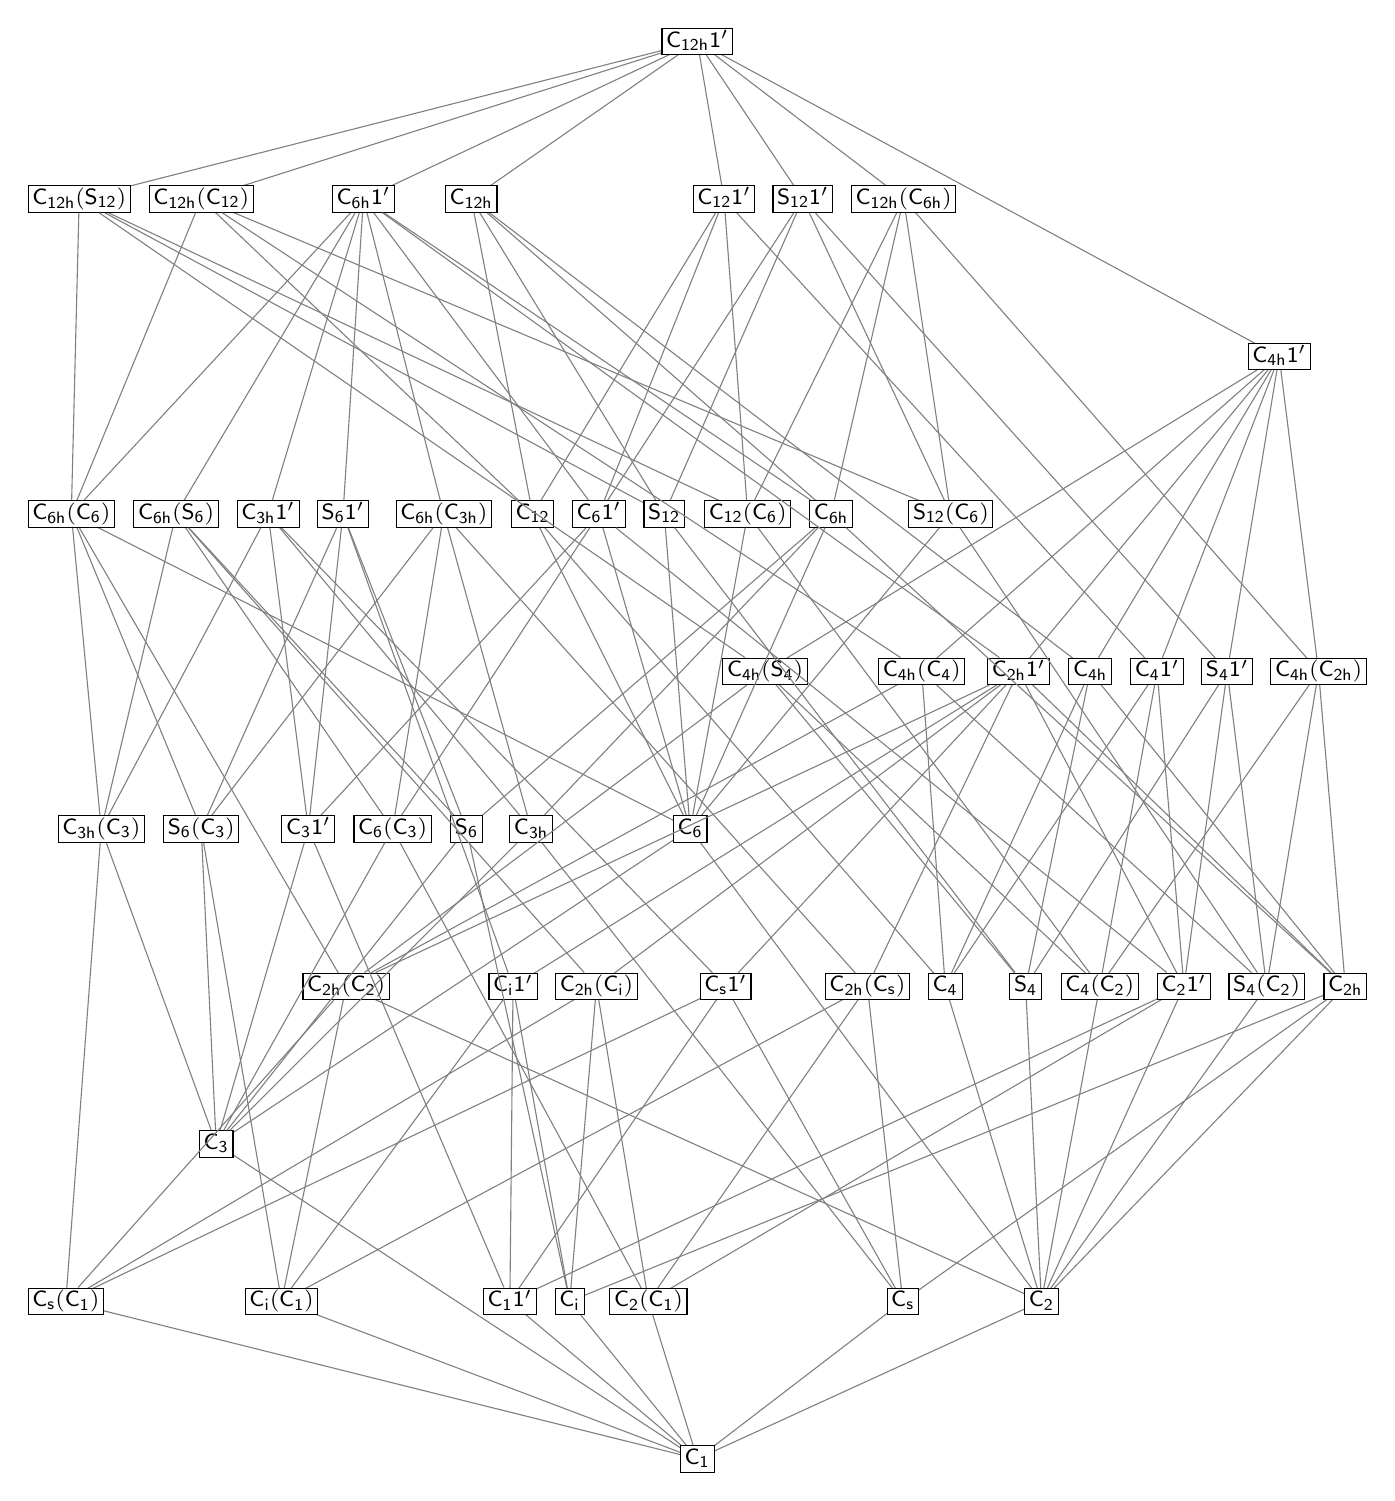
\begin{tikzpicture}[x=1cm, y=2.000cm,
  every node/.style={fill=white, font=\footnotesize, inner xsep=1.5pt, inner ysep=1.2pt, text height=5.6pt, text depth=1.6pt},
  normal/.style={draw, line width=0.4pt}, cover/.style={black!50, line width=0.4pt}]
\draw[cover] (0.00,0) -- (4.37,1);
\draw[cover] (0.00,0) -- (-1.62,1);
\draw[cover] (0.00,0) -- (2.61,1);
\draw[cover] (0.00,0) -- (-2.38,1);
\draw[cover] (0.00,0) -- (-0.62,1);
\draw[cover] (0.00,0) -- (-5.28,1);
\draw[cover] (0.00,0) -- (-8.02,1);
\draw[cover] (0.00,0) -- (-6.11,2);
\draw[cover] (4.37,1) -- (3.15,3);
\draw[cover] (4.37,1) -- (8.23,3);
\draw[cover] (-1.62,1) -- (8.23,3);
\draw[cover] (2.61,1) -- (8.23,3);
\draw[cover] (4.37,1) -- (4.17,3);
\draw[cover] (4.37,1) -- (6.18,3);
\draw[cover] (-2.38,1) -- (6.18,3);
\draw[cover] (-0.62,1) -- (6.18,3);
\draw[cover] (-1.62,1) -- (-2.34,3);
\draw[cover] (-2.38,1) -- (-2.34,3);
\draw[cover] (-5.28,1) -- (-2.34,3);
\draw[cover] (2.61,1) -- (0.36,3);
\draw[cover] (-2.38,1) -- (0.36,3);
\draw[cover] (-8.02,1) -- (0.36,3);
\draw[cover] (4.37,1) -- (5.11,3);
\draw[cover] (4.37,1) -- (-4.46,3);
\draw[cover] (-5.28,1) -- (-4.46,3);
\draw[cover] (-1.62,1) -- (-1.28,3);
\draw[cover] (-0.62,1) -- (-1.28,3);
\draw[cover] (-8.02,1) -- (-1.28,3);
\draw[cover] (2.61,1) -- (2.16,3);
\draw[cover] (-0.62,1) -- (2.16,3);
\draw[cover] (-5.28,1) -- (2.16,3);
\draw[cover] (4.37,1) -- (7.23,3);
\draw[cover] (4.37,1) -- (-0.09,4);
\draw[cover] (-6.11,2) -- (-0.09,4);
\draw[cover] (2.61,1) -- (-2.11,4);
\draw[cover] (-6.11,2) -- (-4.94,4);
\draw[cover] (-0.62,1) -- (-3.87,4);
\draw[cover] (-5.28,1) -- (-6.30,4);
\draw[cover] (-6.11,2) -- (-6.30,4);
\draw[cover] (-8.02,1) -- (-7.57,4);
\draw[cover] (-6.11,2) -- (-7.57,4);
\draw[cover] (3.15,3) -- (4.99,5);
\draw[cover] (8.23,3) -- (4.99,5);
\draw[cover] (4.17,3) -- (4.99,5);
\draw[cover] (3.15,3) -- (5.84,5);
\draw[cover] (6.18,3) -- (5.84,5);
\draw[cover] (5.11,3) -- (5.84,5);
\draw[cover] (8.23,3) -- (4.08,5);
\draw[cover] (6.18,3) -- (4.08,5);
\draw[cover] (-2.34,3) -- (4.08,5);
\draw[cover] (0.36,3) -- (4.08,5);
\draw[cover] (-1.28,3) -- (4.08,5);
\draw[cover] (2.16,3) -- (4.08,5);
\draw[cover] (4.17,3) -- (6.73,5);
\draw[cover] (6.18,3) -- (6.73,5);
\draw[cover] (7.23,3) -- (6.73,5);
\draw[cover] (3.15,3) -- (2.85,5);
\draw[cover] (-4.46,3) -- (2.85,5);
\draw[cover] (7.23,3) -- (2.85,5);
\draw[cover] (8.23,3) -- (7.89,5);
\draw[cover] (5.11,3) -- (7.89,5);
\draw[cover] (7.23,3) -- (7.89,5);
\draw[cover] (4.17,3) -- (0.86,5);
\draw[cover] (5.11,3) -- (0.86,5);
\draw[cover] (3.15,3) -- (-2.09,6);
\draw[cover] (-0.09,4) -- (-2.09,6);
\draw[cover] (-2.93,4) -- (1.70,6);
\draw[cover] (-2.11,4) -- (1.70,6);
\draw[cover] (-0.09,4) -- (-0.42,6);
\draw[cover] (-0.09,4) -- (-1.25,6);
\draw[cover] (-4.94,4) -- (-1.25,6);
\draw[cover] (-3.87,4) -- (-1.25,6);
\draw[cover] (-2.93,4) -- (-4.50,6);
\draw[cover] (-4.94,4) -- (-4.50,6);
\draw[cover] (-6.30,4) -- (-4.50,6);
\draw[cover] (0.36,3) -- (-5.45,6);
\draw[cover] (-2.11,4) -- (-5.45,6);
\draw[cover] (-4.94,4) -- (-5.45,6);
\draw[cover] (-7.57,4) -- (-5.45,6);
\draw[cover] (5.11,3) -- (0.64,6);
\draw[cover] (-0.09,4) -- (0.64,6);
\draw[cover] (-4.46,3) -- (-7.95,6);
\draw[cover] (-0.09,4) -- (-7.95,6);
\draw[cover] (-6.30,4) -- (-7.95,6);
\draw[cover] (-7.57,4) -- (-7.95,6);
\draw[cover] (-2.93,4) -- (-6.62,6);
\draw[cover] (-3.87,4) -- (-6.62,6);
\draw[cover] (-7.57,4) -- (-6.62,6);
\draw[cover] (2.16,3) -- (-3.22,6);
\draw[cover] (-2.11,4) -- (-3.22,6);
\draw[cover] (-3.87,4) -- (-3.22,6);
\draw[cover] (-6.30,4) -- (-3.22,6);
\draw[cover] (-0.09,4) -- (3.22,6);
\draw[cover] (4.99,5) -- (7.39,7);
\draw[cover] (5.84,5) -- (7.39,7);
\draw[cover] (4.08,5) -- (7.39,7);
\draw[cover] (6.73,5) -- (7.39,7);
\draw[cover] (2.85,5) -- (7.39,7);
\draw[cover] (7.89,5) -- (7.39,7);
\draw[cover] (0.86,5) -- (7.39,7);
\draw[cover] (4.99,5) -- (-2.87,8);
\draw[cover] (-2.09,6) -- (-2.87,8);
\draw[cover] (1.70,6) -- (-2.87,8);
\draw[cover] (-0.42,6) -- (-2.87,8);
\draw[cover] (5.84,5) -- (0.34,8);
\draw[cover] (-2.09,6) -- (0.34,8);
\draw[cover] (-1.25,6) -- (0.34,8);
\draw[cover] (0.64,6) -- (0.34,8);
\draw[cover] (1.70,6) -- (-4.24,8);
\draw[cover] (-1.25,6) -- (-4.24,8);
\draw[cover] (-4.50,6) -- (-4.24,8);
\draw[cover] (-5.45,6) -- (-4.24,8);
\draw[cover] (-7.95,6) -- (-4.24,8);
\draw[cover] (-6.62,6) -- (-4.24,8);
\draw[cover] (-3.22,6) -- (-4.24,8);
\draw[cover] (6.73,5) -- (1.34,8);
\draw[cover] (-0.42,6) -- (1.34,8);
\draw[cover] (-1.25,6) -- (1.34,8);
\draw[cover] (3.22,6) -- (1.34,8);
\draw[cover] (-2.09,6) -- (-6.30,8);
\draw[cover] (-7.95,6) -- (-6.30,8);
\draw[cover] (3.22,6) -- (-6.30,8);
\draw[cover] (7.89,5) -- (2.62,8);
\draw[cover] (1.70,6) -- (2.62,8);
\draw[cover] (0.64,6) -- (2.62,8);
\draw[cover] (3.22,6) -- (2.62,8);
\draw[cover] (-0.42,6) -- (-7.85,8);
\draw[cover] (0.64,6) -- (-7.85,8);
\draw[cover] (-7.95,6) -- (-7.85,8);
\draw[cover] (7.39,7) -- (0.00,9);
\draw[cover] (-2.87,8) -- (0.00,9);
\draw[cover] (0.34,8) -- (0.00,9);
\draw[cover] (-4.24,8) -- (0.00,9);
\draw[cover] (1.34,8) -- (0.00,9);
\draw[cover] (-6.30,8) -- (0.00,9);
\draw[cover] (2.62,8) -- (0.00,9);
\draw[cover] (-7.85,8) -- (0.00,9);
\node[normal] (n00) at (0.00,0) {$\grp{C_{1}}$};
\node[normal] (n01) at (4.37,1) {$\grp{C_{2}}$};
\node[normal] (n02) at (-1.62,1) {$\grp{C_{i}}$};
\node[normal] (n03) at (2.61,1) {$\grp{C_{s}}$};
\node[normal] (n04) at (-2.38,1) {$\grp{C_{1}1'}$};
\node[normal] (n05) at (-0.62,1) {$\grp{C_{2}}(\grp{C_{1}})$};
\node[normal] (n06) at (-5.28,1) {$\grp{C_{i}}(\grp{C_{1}})$};
\node[normal] (n07) at (-8.02,1) {$\grp{C_{s}}(\grp{C_{1}})$};
\node[normal] (n08) at (-6.11,2) {$\grp{C_{3}}$};
\node[normal] (n09) at (3.15,3) {$\grp{C_{4}}$};
\node[normal] (n10) at (8.23,3) {$\grp{C_{2h}}$};
\node[normal] (n11) at (4.17,3) {$\grp{S_{4}}$};
\node[normal] (n12) at (6.18,3) {$\grp{C_{2}1'}$};
\node[normal] (n13) at (-2.34,3) {$\grp{C_{i}1'}$};
\node[normal] (n14) at (0.36,3) {$\grp{C_{s}1'}$};
\node[normal] (n15) at (5.11,3) {$\grp{C_{4}}(\grp{C_{2}})$};
\node[normal] (n16) at (-4.46,3) {$\grp{C_{2h}}(\grp{C_{2}})$};
\node[normal] (n17) at (-1.28,3) {$\grp{C_{2h}}(\grp{C_{i}})$};
\node[normal] (n18) at (2.16,3) {$\grp{C_{2h}}(\grp{C_{s}})$};
\node[normal] (n19) at (7.23,3) {$\grp{S_{4}}(\grp{C_{2}})$};
\node[normal] (n20) at (-0.09,4) {$\grp{C_{6}}$};
\node[normal] (n21) at (-2.93,4) {$\grp{S_{6}}$};
\node[normal] (n22) at (-2.11,4) {$\grp{C_{3h}}$};
\node[normal] (n23) at (-4.94,4) {$\grp{C_{3}1'}$};
\node[normal] (n24) at (-3.87,4) {$\grp{C_{6}}(\grp{C_{3}})$};
\node[normal] (n25) at (-6.30,4) {$\grp{S_{6}}(\grp{C_{3}})$};
\node[normal] (n26) at (-7.57,4) {$\grp{C_{3h}}(\grp{C_{3}})$};
\node[normal] (n27) at (4.99,5) {$\grp{C_{4h}}$};
\node[normal] (n28) at (5.84,5) {$\grp{C_{4}1'}$};
\node[normal] (n29) at (4.08,5) {$\grp{C_{2h}1'}$};
\node[normal] (n30) at (6.73,5) {$\grp{S_{4}1'}$};
\node[normal] (n31) at (2.85,5) {$\grp{C_{4h}}(\grp{C_{4}})$};
\node[normal] (n32) at (7.89,5) {$\grp{C_{4h}}(\grp{C_{2h}})$};
\node[normal] (n33) at (0.86,5) {$\grp{C_{4h}}(\grp{S_{4}})$};
\node[normal] (n34) at (-2.09,6) {$\grp{C_{12}}$};
\node[normal] (n35) at (1.70,6) {$\grp{C_{6h}}$};
\node[normal] (n36) at (-0.42,6) {$\grp{S_{12}}$};
\node[normal] (n37) at (-1.25,6) {$\grp{C_{6}1'}$};
\node[normal] (n38) at (-4.50,6) {$\grp{S_{6}1'}$};
\node[normal] (n39) at (-5.45,6) {$\grp{C_{3h}1'}$};
\node[normal] (n40) at (0.64,6) {$\grp{C_{12}}(\grp{C_{6}})$};
\node[normal] (n41) at (-7.95,6) {$\grp{C_{6h}}(\grp{C_{6}})$};
\node[normal] (n42) at (-6.62,6) {$\grp{C_{6h}}(\grp{S_{6}})$};
\node[normal] (n43) at (-3.22,6) {$\grp{C_{6h}}(\grp{C_{3h}})$};
\node[normal] (n44) at (3.22,6) {$\grp{S_{12}}(\grp{C_{6}})$};
\node[normal] (n45) at (7.39,7) {$\grp{C_{4h}1'}$};
\node[normal] (n46) at (-2.87,8) {$\grp{C_{12h}}$};
\node[normal] (n47) at (0.34,8) {$\grp{C_{12}1'}$};
\node[normal] (n48) at (-4.24,8) {$\grp{C_{6h}1'}$};
\node[normal] (n49) at (1.34,8) {$\grp{S_{12}1'}$};
\node[normal] (n50) at (-6.30,8) {$\grp{C_{12h}}(\grp{C_{12}})$};
\node[normal] (n51) at (2.62,8) {$\grp{C_{12h}}(\grp{C_{6h}})$};
\node[normal] (n52) at (-7.85,8) {$\grp{C_{12h}}(\grp{S_{12}})$};
\node[normal] (n53) at (0.00,9) {$\grp{C_{12h}1'}$};
\draw[cover] (n07) -- (n16);
\draw[cover] (n02) -- (n21);
\draw[cover] (n08) -- (n21);
\draw[cover] (n08) -- (n22);
\draw[cover] (n04) -- (n23);
\draw[cover] (n08) -- (n24);
\draw[cover] (n16) -- (n29);
\draw[cover] (n16) -- (n33);
\draw[cover] (n10) -- (n35);
\draw[cover] (n20) -- (n35);
\draw[cover] (n11) -- (n36);
\draw[cover] (n12) -- (n37);
\draw[cover] (n13) -- (n38);
\draw[cover] (n17) -- (n42);
\draw[cover] (n19) -- (n44);
\draw[cover] (n29) -- (n48);
\draw[cover] (n31) -- (n50);
\draw[cover] (n33) -- (n52);
\end{tikzpicture}
\end{center}
{\small\begin{longtable}{@{}llrrlll@{}}\toprule
subgrp & type & order & conjugates & normal & normalizer & centralizer\\\midrule\endhead
\bottomrule\endfoot\endlastfoot
\href{../../../rotation/data/pdf/C1.pdf}{$\grp{C_{1}}$} & I & 1 & 1 & yes & \href{C12h-1p.pdf}{$\grp{C_{12h}1'}$} & \href{C12h-1p.pdf}{$\grp{C_{12h}1'}$}\\*
\href{../../../rotation/data/pdf/C2.pdf}{$\grp{C_{2}}$} & I & 2 & 1 & yes & \href{C12h-1p.pdf}{$\grp{C_{12h}1'}$} & \href{C12h-1p.pdf}{$\grp{C_{12h}1'}$}\\
\href{../../../rotation/data/pdf/S2.pdf}{$\grp{C_{i}}$} & I & 2 & 1 & yes & \href{C12h-1p.pdf}{$\grp{C_{12h}1'}$} & \href{C12h-1p.pdf}{$\grp{C_{12h}1'}$}\\
\href{../../../rotation/data/pdf/C1v.pdf}{$\grp{C_{s}}$} & I & 2 & 1 & yes & \href{C12h-1p.pdf}{$\grp{C_{12h}1'}$} & \href{C12h-1p.pdf}{$\grp{C_{12h}1'}$}\\
\href{C1-1p.pdf}{$\grp{C_{1}1'}$} & II & 2 & 1 & yes & \href{C12h-1p.pdf}{$\grp{C_{12h}1'}$} & \href{C12h-1p.pdf}{$\grp{C_{12h}1'}$}\\
\href{C2-C1.pdf}{$\grp{C_{2}}(\grp{C_{1}})$} & III & 2 & 1 & yes & \href{C12h-1p.pdf}{$\grp{C_{12h}1'}$} & \href{C12h-1p.pdf}{$\grp{C_{12h}1'}$}\\
\href{S2-C1.pdf}{$\grp{C_{i}}(\grp{C_{1}})$} & III & 2 & 1 & yes & \href{C12h-1p.pdf}{$\grp{C_{12h}1'}$} & \href{C12h-1p.pdf}{$\grp{C_{12h}1'}$}\\
\href{C1v-C1.pdf}{$\grp{C_{s}}(\grp{C_{1}})$} & III & 2 & 1 & yes & \href{C12h-1p.pdf}{$\grp{C_{12h}1'}$} & \href{C12h-1p.pdf}{$\grp{C_{12h}1'}$}\\
\href{../../../rotation/data/pdf/C3.pdf}{$\grp{C_{3}}$} & I & 3 & 1 & yes & \href{C12h-1p.pdf}{$\grp{C_{12h}1'}$} & \href{C12h-1p.pdf}{$\grp{C_{12h}1'}$}\\
\href{../../../rotation/data/pdf/C4.pdf}{$\grp{C_{4}}$} & I & 4 & 1 & yes & \href{C12h-1p.pdf}{$\grp{C_{12h}1'}$} & \href{C12h-1p.pdf}{$\grp{C_{12h}1'}$}\\
\href{../../../rotation/data/pdf/S4.pdf}{$\grp{S_{4}}$} & I & 4 & 1 & yes & \href{C12h-1p.pdf}{$\grp{C_{12h}1'}$} & \href{C12h-1p.pdf}{$\grp{C_{12h}1'}$}\\
\href{../../../rotation/data/pdf/C2h.pdf}{$\grp{C_{2h}}$} & I & 4 & 1 & yes & \href{C12h-1p.pdf}{$\grp{C_{12h}1'}$} & \href{C12h-1p.pdf}{$\grp{C_{12h}1'}$}\\
\href{C2-1p.pdf}{$\grp{C_{2}1'}$} & II & 4 & 1 & yes & \href{C12h-1p.pdf}{$\grp{C_{12h}1'}$} & \href{C12h-1p.pdf}{$\grp{C_{12h}1'}$}\\
\href{S2-1p.pdf}{$\grp{C_{i}1'}$} & II & 4 & 1 & yes & \href{C12h-1p.pdf}{$\grp{C_{12h}1'}$} & \href{C12h-1p.pdf}{$\grp{C_{12h}1'}$}\\
\href{C1v-1p.pdf}{$\grp{C_{s}1'}$} & II & 4 & 1 & yes & \href{C12h-1p.pdf}{$\grp{C_{12h}1'}$} & \href{C12h-1p.pdf}{$\grp{C_{12h}1'}$}\\
\href{C4-C2.pdf}{$\grp{C_{4}}(\grp{C_{2}})$} & III & 4 & 1 & yes & \href{C12h-1p.pdf}{$\grp{C_{12h}1'}$} & \href{C12h-1p.pdf}{$\grp{C_{12h}1'}$}\\
\href{S4-C2.pdf}{$\grp{S_{4}}(\grp{C_{2}})$} & III & 4 & 1 & yes & \href{C12h-1p.pdf}{$\grp{C_{12h}1'}$} & \href{C12h-1p.pdf}{$\grp{C_{12h}1'}$}\\
\href{C2h-C2.pdf}{$\grp{C_{2h}}(\grp{C_{2}})$} & III & 4 & 1 & yes & \href{C12h-1p.pdf}{$\grp{C_{12h}1'}$} & \href{C12h-1p.pdf}{$\grp{C_{12h}1'}$}\\
\href{C2h-S2.pdf}{$\grp{C_{2h}}(\grp{C_{i}})$} & III & 4 & 1 & yes & \href{C12h-1p.pdf}{$\grp{C_{12h}1'}$} & \href{C12h-1p.pdf}{$\grp{C_{12h}1'}$}\\
\href{C2h-C1v.pdf}{$\grp{C_{2h}}(\grp{C_{s}})$} & III & 4 & 1 & yes & \href{C12h-1p.pdf}{$\grp{C_{12h}1'}$} & \href{C12h-1p.pdf}{$\grp{C_{12h}1'}$}\\
\href{../../../rotation/data/pdf/C6.pdf}{$\grp{C_{6}}$} & I & 6 & 1 & yes & \href{C12h-1p.pdf}{$\grp{C_{12h}1'}$} & \href{C12h-1p.pdf}{$\grp{C_{12h}1'}$}\\
\href{../../../rotation/data/pdf/S6.pdf}{$\grp{S_{6}}$} & I & 6 & 1 & yes & \href{C12h-1p.pdf}{$\grp{C_{12h}1'}$} & \href{C12h-1p.pdf}{$\grp{C_{12h}1'}$}\\
\href{../../../rotation/data/pdf/C3h.pdf}{$\grp{C_{3h}}$} & I & 6 & 1 & yes & \href{C12h-1p.pdf}{$\grp{C_{12h}1'}$} & \href{C12h-1p.pdf}{$\grp{C_{12h}1'}$}\\
\href{C3-1p.pdf}{$\grp{C_{3}1'}$} & II & 6 & 1 & yes & \href{C12h-1p.pdf}{$\grp{C_{12h}1'}$} & \href{C12h-1p.pdf}{$\grp{C_{12h}1'}$}\\
\href{C6-C3.pdf}{$\grp{C_{6}}(\grp{C_{3}})$} & III & 6 & 1 & yes & \href{C12h-1p.pdf}{$\grp{C_{12h}1'}$} & \href{C12h-1p.pdf}{$\grp{C_{12h}1'}$}\\
\href{S6-C3.pdf}{$\grp{S_{6}}(\grp{C_{3}})$} & III & 6 & 1 & yes & \href{C12h-1p.pdf}{$\grp{C_{12h}1'}$} & \href{C12h-1p.pdf}{$\grp{C_{12h}1'}$}\\
\href{C3h-C3.pdf}{$\grp{C_{3h}}(\grp{C_{3}})$} & III & 6 & 1 & yes & \href{C12h-1p.pdf}{$\grp{C_{12h}1'}$} & \href{C12h-1p.pdf}{$\grp{C_{12h}1'}$}\\
\href{../../../rotation/data/pdf/C4h.pdf}{$\grp{C_{4h}}$} & I & 8 & 1 & yes & \href{C12h-1p.pdf}{$\grp{C_{12h}1'}$} & \href{C12h-1p.pdf}{$\grp{C_{12h}1'}$}\\
\href{C4-1p.pdf}{$\grp{C_{4}1'}$} & II & 8 & 1 & yes & \href{C12h-1p.pdf}{$\grp{C_{12h}1'}$} & \href{C12h-1p.pdf}{$\grp{C_{12h}1'}$}\\
\href{S4-1p.pdf}{$\grp{S_{4}1'}$} & II & 8 & 1 & yes & \href{C12h-1p.pdf}{$\grp{C_{12h}1'}$} & \href{C12h-1p.pdf}{$\grp{C_{12h}1'}$}\\
\href{C2h-1p.pdf}{$\grp{C_{2h}1'}$} & II & 8 & 1 & yes & \href{C12h-1p.pdf}{$\grp{C_{12h}1'}$} & \href{C12h-1p.pdf}{$\grp{C_{12h}1'}$}\\
\href{C4h-C4.pdf}{$\grp{C_{4h}}(\grp{C_{4}})$} & III & 8 & 1 & yes & \href{C12h-1p.pdf}{$\grp{C_{12h}1'}$} & \href{C12h-1p.pdf}{$\grp{C_{12h}1'}$}\\
\href{C4h-S4.pdf}{$\grp{C_{4h}}(\grp{S_{4}})$} & III & 8 & 1 & yes & \href{C12h-1p.pdf}{$\grp{C_{12h}1'}$} & \href{C12h-1p.pdf}{$\grp{C_{12h}1'}$}\\
\href{C4h-C2h.pdf}{$\grp{C_{4h}}(\grp{C_{2h}})$} & III & 8 & 1 & yes & \href{C12h-1p.pdf}{$\grp{C_{12h}1'}$} & \href{C12h-1p.pdf}{$\grp{C_{12h}1'}$}\\
\href{../../../rotation/data/pdf/C12.pdf}{$\grp{C_{12}}$} & I & 12 & 1 & yes & \href{C12h-1p.pdf}{$\grp{C_{12h}1'}$} & \href{C12h-1p.pdf}{$\grp{C_{12h}1'}$}\\
\href{../../../rotation/data/pdf/S12.pdf}{$\grp{S_{12}}$} & I & 12 & 1 & yes & \href{C12h-1p.pdf}{$\grp{C_{12h}1'}$} & \href{C12h-1p.pdf}{$\grp{C_{12h}1'}$}\\
\href{../../../rotation/data/pdf/C6h.pdf}{$\grp{C_{6h}}$} & I & 12 & 1 & yes & \href{C12h-1p.pdf}{$\grp{C_{12h}1'}$} & \href{C12h-1p.pdf}{$\grp{C_{12h}1'}$}\\
\href{C6-1p.pdf}{$\grp{C_{6}1'}$} & II & 12 & 1 & yes & \href{C12h-1p.pdf}{$\grp{C_{12h}1'}$} & \href{C12h-1p.pdf}{$\grp{C_{12h}1'}$}\\
\href{S6-1p.pdf}{$\grp{S_{6}1'}$} & II & 12 & 1 & yes & \href{C12h-1p.pdf}{$\grp{C_{12h}1'}$} & \href{C12h-1p.pdf}{$\grp{C_{12h}1'}$}\\
\href{C3h-1p.pdf}{$\grp{C_{3h}1'}$} & II & 12 & 1 & yes & \href{C12h-1p.pdf}{$\grp{C_{12h}1'}$} & \href{C12h-1p.pdf}{$\grp{C_{12h}1'}$}\\
\href{C12-C6.pdf}{$\grp{C_{12}}(\grp{C_{6}})$} & III & 12 & 1 & yes & \href{C12h-1p.pdf}{$\grp{C_{12h}1'}$} & \href{C12h-1p.pdf}{$\grp{C_{12h}1'}$}\\
\href{S12-C6.pdf}{$\grp{S_{12}}(\grp{C_{6}})$} & III & 12 & 1 & yes & \href{C12h-1p.pdf}{$\grp{C_{12h}1'}$} & \href{C12h-1p.pdf}{$\grp{C_{12h}1'}$}\\
\href{C6h-C6.pdf}{$\grp{C_{6h}}(\grp{C_{6}})$} & III & 12 & 1 & yes & \href{C12h-1p.pdf}{$\grp{C_{12h}1'}$} & \href{C12h-1p.pdf}{$\grp{C_{12h}1'}$}\\
\href{C6h-S6.pdf}{$\grp{C_{6h}}(\grp{S_{6}})$} & III & 12 & 1 & yes & \href{C12h-1p.pdf}{$\grp{C_{12h}1'}$} & \href{C12h-1p.pdf}{$\grp{C_{12h}1'}$}\\
\href{C6h-C3h.pdf}{$\grp{C_{6h}}(\grp{C_{3h}})$} & III & 12 & 1 & yes & \href{C12h-1p.pdf}{$\grp{C_{12h}1'}$} & \href{C12h-1p.pdf}{$\grp{C_{12h}1'}$}\\
\href{C4h-1p.pdf}{$\grp{C_{4h}1'}$} & II & 16 & 1 & yes & \href{C12h-1p.pdf}{$\grp{C_{12h}1'}$} & \href{C12h-1p.pdf}{$\grp{C_{12h}1'}$}\\
\href{../../../rotation/data/pdf/C12h.pdf}{$\grp{C_{12h}}$} & I & 24 & 1 & yes & \href{C12h-1p.pdf}{$\grp{C_{12h}1'}$} & \href{C12h-1p.pdf}{$\grp{C_{12h}1'}$}\\
\href{C12-1p.pdf}{$\grp{C_{12}1'}$} & II & 24 & 1 & yes & \href{C12h-1p.pdf}{$\grp{C_{12h}1'}$} & \href{C12h-1p.pdf}{$\grp{C_{12h}1'}$}\\
\href{S12-1p.pdf}{$\grp{S_{12}1'}$} & II & 24 & 1 & yes & \href{C12h-1p.pdf}{$\grp{C_{12h}1'}$} & \href{C12h-1p.pdf}{$\grp{C_{12h}1'}$}\\
\href{C6h-1p.pdf}{$\grp{C_{6h}1'}$} & II & 24 & 1 & yes & \href{C12h-1p.pdf}{$\grp{C_{12h}1'}$} & \href{C12h-1p.pdf}{$\grp{C_{12h}1'}$}\\
\href{C12h-C12.pdf}{$\grp{C_{12h}}(\grp{C_{12}})$} & III & 24 & 1 & yes & \href{C12h-1p.pdf}{$\grp{C_{12h}1'}$} & \href{C12h-1p.pdf}{$\grp{C_{12h}1'}$}\\
\href{C12h-S12.pdf}{$\grp{C_{12h}}(\grp{S_{12}})$} & III & 24 & 1 & yes & \href{C12h-1p.pdf}{$\grp{C_{12h}1'}$} & \href{C12h-1p.pdf}{$\grp{C_{12h}1'}$}\\
\href{C12h-C6h.pdf}{$\grp{C_{12h}}(\grp{C_{6h}})$} & III & 24 & 1 & yes & \href{C12h-1p.pdf}{$\grp{C_{12h}1'}$} & \href{C12h-1p.pdf}{$\grp{C_{12h}1'}$}\\*
\href{C12h-1p.pdf}{$\grp{C_{12h}1'}$} & II & 48 & 1 & yes & \href{C12h-1p.pdf}{$\grp{C_{12h}1'}$} & \href{C12h-1p.pdf}{$\grp{C_{12h}1'}$}\\
\bottomrule\end{longtable}}
\needspace{171pt}
\partbox{Angular momentum}
\section{Subduction from \texorpdfstring{$\grp{O(3)1'}$}{O(3)1\unichar{8242}}}\label{s:subduction_o3}
Conventions: \href{../../CONVENTIONS.pdf}{CONVENTIONS.pdf}, sections \href{../../../rotation/CONVENTIONS.pdf\#conv.11}{11} and \href{../../CONVENTIONS.pdf\#conv.33.1}{33.1}.
\leavevmode\label{n:index.J}\label{n:index.parity}The irrep $\irrJp{J}{p}$ of $\grp{O(3)1'}$ has angular momentum $J$ and parity $p$ ($\ptag{g}$ for $p = +1$, $\ptag{u}$ for $p = -1$), and time reversal acts on it as on its kets (\href{../../CONVENTIONS.pdf}{CONVENTIONS.pdf}, section \href{../../CONVENTIONS.pdf\#conv.31.1}{31.1}). A row is an angular momentum $J \le 6$. A row gives the multiplicity of each corepresentation of $\grp{C_{12h}1'}$ in the restriction of $\irrJp{J}{p}$ to $\grp{C_{12h}1'}$. A corepresentation occurs as often as its first irrep occurs in the restriction to $\grp{C_{12h}}$ (the section Subduction from $\grp{O(3)}$ of the document of \href{../../../rotation/data/pdf/C12h.pdf}{$\grp{C_{12h}}$}), half as often in case (b).
\needspace{149pt}
\paragraph{Parity $\ptag{g}$ ($p = +1$).}
{\small\begin{longtable}{@{}rrrrrrrr@{}}\toprule
$J$ & $\irr{a}_{\ptag{g}}$ & $\irr{b}_{\ptag{g}}$ & $\conjpair{1}\irr{e}_{1\ptag{g}}\,\conjpair{2}\irr{e}_{1\ptag{g}}$ & $\conjpair{1}\irr{e}_{2\ptag{g}}\,\conjpair{2}\irr{e}_{2\ptag{g}}$ & $\conjpair{1}\irr{e}_{3\ptag{g}}\,\conjpair{2}\irr{e}_{3\ptag{g}}$ & $\conjpair{1}\irr{e}_{4\ptag{g}}\,\conjpair{2}\irr{e}_{4\ptag{g}}$ & $\conjpair{1}\irr{e}_{5\ptag{g}}\,\conjpair{2}\irr{e}_{5\ptag{g}}$\\\midrule\endhead
\bottomrule\endfoot\endlastfoot
0 & 1 & 0 & 0 & 0 & 0 & 0 & 0\\*
1 & 1 & 0 & 1 & 0 & 0 & 0 & 0\\*
2 & 1 & 0 & 1 & 1 & 0 & 0 & 0\\*
3 & 1 & 0 & 1 & 1 & 1 & 0 & 0\\*
4 & 1 & 0 & 1 & 1 & 1 & 1 & 0\\*
5 & 1 & 0 & 1 & 1 & 1 & 1 & 1\\*
6 & 1 & 2 & 1 & 1 & 1 & 1 & 1\\
\bottomrule\end{longtable}}
\needspace{149pt}
\paragraph{Parity $\ptag{u}$ ($p = -1$).}
{\small\begin{longtable}{@{}rrrrrrrr@{}}\toprule
$J$ & $\irr{a}_{\ptag{u}}$ & $\irr{b}_{\ptag{u}}$ & $\conjpair{1}\irr{e}_{1\ptag{u}}\,\conjpair{2}\irr{e}_{1\ptag{u}}$ & $\conjpair{1}\irr{e}_{2\ptag{u}}\,\conjpair{2}\irr{e}_{2\ptag{u}}$ & $\conjpair{1}\irr{e}_{3\ptag{u}}\,\conjpair{2}\irr{e}_{3\ptag{u}}$ & $\conjpair{1}\irr{e}_{4\ptag{u}}\,\conjpair{2}\irr{e}_{4\ptag{u}}$ & $\conjpair{1}\irr{e}_{5\ptag{u}}\,\conjpair{2}\irr{e}_{5\ptag{u}}$\\\midrule\endhead
\bottomrule\endfoot\endlastfoot
0 & 1 & 0 & 0 & 0 & 0 & 0 & 0\\*
1 & 1 & 0 & 1 & 0 & 0 & 0 & 0\\*
2 & 1 & 0 & 1 & 1 & 0 & 0 & 0\\*
3 & 1 & 0 & 1 & 1 & 1 & 0 & 0\\*
4 & 1 & 0 & 1 & 1 & 1 & 1 & 0\\*
5 & 1 & 0 & 1 & 1 & 1 & 1 & 1\\*
6 & 1 & 2 & 1 & 1 & 1 & 1 & 1\\
\bottomrule\end{longtable}}
\needspace{250pt}
\partbox{Tensors}
\section{Multipoles}\label{s:multipoles}
Conventions: \href{../../CONVENTIONS.pdf}{CONVENTIONS.pdf}, section \href{../../CONVENTIONS.pdf\#conv.35.1}{35.1}.
A row is a rank $J$. \label{n:head.multipole.electric}\label{n:head.multipole.electric.toroidal}A row gives the number of independent multipoles of each kind that $\grp{C_{12h}1'}$ allows. It is the multiplicity in $\irrJp{J}{p}$ of the trivial irrep of $\grp{C_{12h}}$ (the section Subduction from $\grp{O(3)}$ of the document of \href{../../../rotation/data/pdf/C12h.pdf}{$\grp{C_{12h}}$}).
{\small\begin{longtable}{@{}rrr@{}}\toprule
$J$ & electric & electric toroidal\\\midrule\endhead
\bottomrule\endfoot\endlastfoot
0 & 1 & 0\\*
1 & 0 & 1\\*
2 & 1 & 0\\*
3 & 0 & 1\\*
4 & 1 & 0\\
\bottomrule\end{longtable}}
The electric entries at even $J$ count the operators on a spin that $\grp{C_{12h}1'}$ allows (\href{../../CONVENTIONS.pdf}{CONVENTIONS.pdf}, section \href{../../CONVENTIONS.pdf\#conv.35.1}{35.1}).
\needspace{103pt}
\section{Invariants}\label{s:invariants}
Conventions: \href{../../CONVENTIONS.pdf}{CONVENTIONS.pdf}, sections \href{../../CONVENTIONS.pdf\#conv.31.2}{31.2} and \href{../../CONVENTIONS.pdf\#conv.35.1}{35.1}.
The invariant polynomials of $\grp{C_{12h}1'}$ in one vector of a kind are those of its image of that kind (section~\ref{s:identification}), in the section Invariant polynomials of the image's document (\texttt{rings}).
\leavevmode\label{n:index.degree.polar}\label{n:index.degree.axial}A row is a degree $a$ in a polar vector even under time reversal. A row gives the number of linearly independent invariants of degree $a$ in it and $b$ in an axial vector odd under time reversal, for $a + b \le 6$.
{\small\begin{longtable}{@{}rrrrrr@{}}\toprule
$a$ & $b = 1$ & $b = 2$ & $b = 3$ & $b = 4$ & $b = 5$\\\midrule\endhead
\bottomrule\endfoot\endlastfoot
1 & 0 & 0 & 0 & 0 & 0\\*
2 & 0 & 8 & 0 & 14 & \\*
3 & 0 & 0 & 0 &  & \\*
4 & 0 & 14 &  &  & \\*
5 & 0 &  &  &  & \\
\bottomrule\end{longtable}}
\leavevmode\label{n:local.component.polar}\label{n:local.component.axial}The record holds their bases for $a + b \le 4$ (\texttt{polynomials}), in the components $u_{x}$, $u_{y}$, $u_{z}$ of the polar vector and $v_{x}$, $v_{y}$, $v_{z}$ of the axial vector. \label{n:head.polynomial}A row is an invariant of the reduced row echelon basis of its degrees (\href{../../CONVENTIONS.pdf}{CONVENTIONS.pdf}, section \href{../../CONVENTIONS.pdf\#conv.35.1}{35.1}). A row gives its degrees $a$ and $b$ and the invariant (polynomial).
{\small\renewcommand{\arraystretch}{1.2}\begin{longtable}{@{}rrl@{\hspace{18pt}}rrl@{}}\toprule
$a$ & $b$ & polynomial & $a$ & $b$ & polynomial\\\midrule\endhead
\bottomrule\endfoot\endlastfoot
2 & 2 & $u_{x}^{2}v_{x}^{2} + 2u_{x}u_{y}v_{x}v_{y} + u_{y}^{2}v_{y}^{2}$ & 2 & 2 & $u_{x}u_{z}v_{x}v_{z} + u_{y}u_{z}v_{y}v_{z}$\\*
2 & 2 & $u_{x}^{2}v_{x}v_{y} - u_{x}u_{y}v_{x}^{2} + u_{x}u_{y}v_{y}^{2} - u_{y}^{2}v_{x}v_{y}$ & 2 & 2 & $u_{x}u_{z}v_{y}v_{z} - u_{y}u_{z}v_{x}v_{z}$\\*
2 & 2 & $u_{x}^{2}v_{y}^{2} - 2u_{x}u_{y}v_{x}v_{y} + u_{y}^{2}v_{x}^{2}$ & 2 & 2 & $u_{z}^{2}v_{x}^{2} + u_{z}^{2}v_{y}^{2}$\\*
2 & 2 & $u_{x}^{2}v_{z}^{2} + u_{y}^{2}v_{z}^{2}$ & 2 & 2 & $u_{z}^{2}v_{z}^{2}$\\
\bottomrule\end{longtable}}
\end{document}
